\فصل{نتایج}
\label{chap:results}

\قسمت{تشکیل آرایش چندذره‌ای با طراحی رهاسازی}
\label{sec:results-particle-formation}

آرایش ذرات در کانال مستطیلی دوبعدی به‌صورت عددی بررسی شد.
هندسه و مدل ذره مطابق بخش~\ref{sec:theory-particle-formation} هستند.
همهٔ مکان‌ها، زمان‌ها و فاصله‌های این بخش بی‌بعد هستند.
در هر حالت، هدف رسیدن هم‌زمان مراکز ذرات به نقاط مشخص بود.
خطای نهایی و کمینهٔ فاصله طبق رابطهٔ~\eqref{eq:validation-formation-errors} محاسبه شدند.

\زیرقسمت{تشکیل یک آرایش ساده}
\label{sec:results-formation-triangle}

مثلث، نمونهٔ پایه برای بررسی آرایش با سه ذره است.
دو ذره از دیوارهٔ پایین و یک ذره از بالا رها شدند.
مکان رهاسازی هر ذره روی دیوارهٔ خودش مستقل انتخاب شد.
دو ذرهٔ پایین تقریباً در زمان $t^*=0.2500$ رها شدند.
ذرهٔ بالا در زمان $t^*=0.2894$ رها شد.
هر سه مسیر در زمان هدف $T^*=0.3462$ ارزیابی شدند.

دو پنل نخست شکل~\ref{fig:results-formation-basic} مسیرها و مراکز نهایی مثلث را نشان می‌دهند.
این نمونه با تنظیمات اجرای پیشین و وزن‌های ثابت دوباره محاسبه شد.
بیشینهٔ خطای نهایی در میدان شبکه برابر $2.67\times10^{-9}$ بود.
در میدان تحلیلی، این خطا به $9.08\times10^{-7}$ رسید.
کمینهٔ فاصلهٔ مراکز در هر دو بازپخش حدود $0.12990$ بود.
این فاصله از آستانهٔ پذیرش $0.026$ بیشتر بود.

\begin{figure}[htbp]
\centering
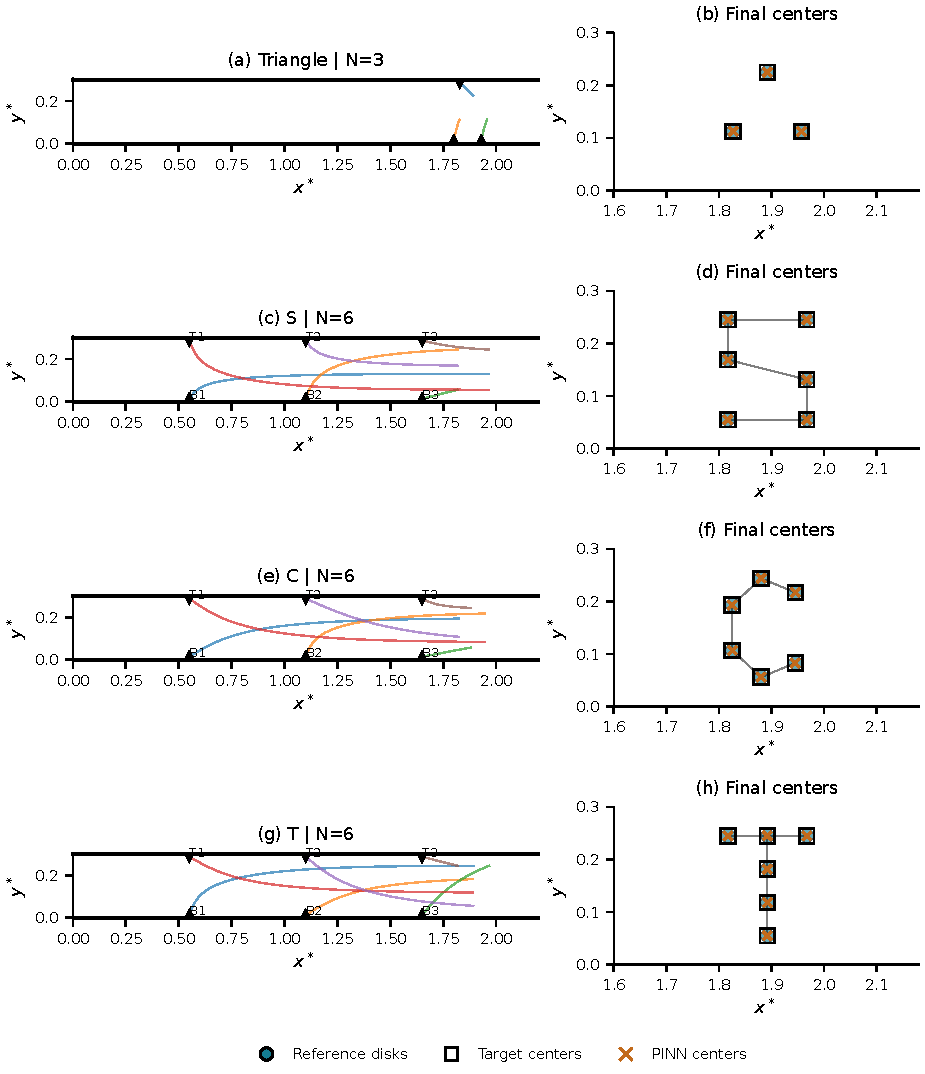
\includegraphics[width=0.95\textwidth,height=0.75\textheight,keepaspectratio]{figs/chapter4/formation-basic-cases.pdf}
\caption{مسیر رهاسازی و مراکز نهایی مثلث و حروف \lr{S}، \lr{C} و \lr{T}.}
\label{fig:results-formation-basic}
\end{figure}

\زیرقسمت{تشکیل حروف \lr{S}، \lr{C} و \lr{T} با شش ایستگاه ثابت}
\label{sec:results-formation-letters}

در هر دیواره، سه ایستگاه در $x^*=0.55,\,1.10,\,1.65$ قرار داشتند.
برای هر حرف، از هر ایستگاه یک ذره رها شد.
سرعت اولیه و زمان رهاسازی برای هر ذره جداگانه تعیین شدند.
سه ردیف پایانی شکل~\ref{fig:results-formation-basic} مسیرهای حروف را نشان می‌دهند.
مراکز نهایی در نمای نزدیک با نقاط هدف مقایسه شده‌اند.

جدول~\ref{tab:results-formation-letters} خطای نهایی و کمینهٔ فاصله را گزارش می‌کند.
بیشینهٔ خطای مرجع در میان حروف، متعلق به حرف \lr{S} بود.
حرف \lr{T} در هر دو بازپخش کمترین فاصلهٔ مراکز را داشت.
کمینهٔ فاصلهٔ مرجع این حرف حدود $0.02746$ بود.
هر سه برنامه در بازپخش عددی معیارهای پذیرش را برآورده کردند.

\begin{table}[htbp]
\centering
\small
\setlength{\tabcolsep}{5pt}
\caption{خطای نهایی و کمینهٔ فاصلهٔ بی‌بعد برای سه حرف.}
\label{tab:results-formation-letters}
\begin{tabular}{@{}lccccc@{}}
\hline
حرف & $T^*$ & $E_{\max,\mathrm{PINN}}^*$ & $E_{\max,\mathrm{ref}}^*$
& $d_{\min,\mathrm{PINN}}^*$ & $d_{\min,\mathrm{ref}}^*$ \\
\hline
\lr{S} & $2.3875$ & $2.073\times10^{-8}$ & $3.768\times10^{-4}$ & $0.0335802$ & $0.0336059$ \\
\lr{C} & $1.8674$ & $1.121\times10^{-8}$ & $1.948\times10^{-4}$ & $0.0348533$ & $0.0348257$ \\
\lr{T} & $2.2739$ & $1.141\times10^{-8}$ & $2.877\times10^{-4}$ & $0.0274005$ & $0.0274613$ \\
\hline
\end{tabular}
\end{table}

اندیس \lr{PINN} به بازپخش با میدان شبکه اشاره دارد.
اندیس \lr{ref} بازپخش مستقل با میدان تحلیلی پوازوی را مشخص می‌کند.
مقدار $T^*$ زمان هدف همان آرایش است.

\زیرقسمت{آرایش اردک و بازپخش مستقل برنامه‌های رهاسازی}
\label{sec:results-formation-ducks}

چهار برنامهٔ ذخیره‌شده برای آرایش اردک دوباره بازپخش شدند.
حالت‌های ۲۰ و ۴۲ ذره‌ای از شش ایستگاه ثابت استفاده کردند.
در این حالت‌ها، هر ایستگاه می‌توانست چند ذره رها کند.
در حالت‌های ۲۸ و ۶۴ ذره‌ای، مکان رهاسازی هر ذره آزاد بود.
هر برنامه با میدان شبکه و میدان تحلیلی پوازوی بازپخش شد.
برنامهٔ رهاسازی هر حالت در هر دو بازپخش یکسان بود.

شکل~\ref{fig:results-formation-ducks} آرایش‌ها را در زمان هدف هر برنامه نشان می‌دهد.
دیسک‌ها اندازهٔ ذرات را با مقیاس هندسی کانال نشان می‌دهند.
جدول~\ref{tab:results-formation-ducks} خطای نهایی و کمینهٔ فاصله را مقایسه می‌کند.

\begin{figure}[htbp]
\centering
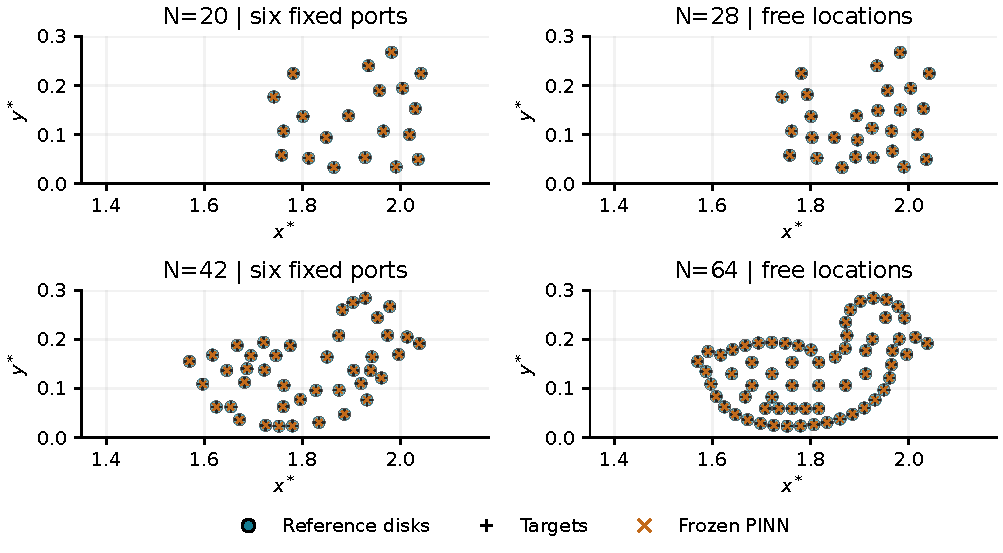
\includegraphics[width=0.95\textwidth]{figs/chapter4/formation-duck-replays.pdf}
% REVIEW-AUDIT Y02 | در زمان هدف | تعداد و نوع رهاسازی هم‌زمان عوض شده‌اند. ارزیابی در زمان هدف است. | پیشنهاد: مقایسهٔ چهار برنامه در زمان هدف هر برنامه | مرور؛ محدودیت مقایسه و افق نتیجه | تطبیق با متن گزارش
\caption{چهار آرایش اردک \ReviewMark{yellow}{Y02-91-1-1}{در زمان هدف} برنامه‌های رهاسازی.}
\label{fig:results-formation-ducks}
\end{figure}

\begin{table}[htbp]
\centering
\small
\setlength{\tabcolsep}{5pt}
\caption{مقایسهٔ بی‌بعد بازپخش شبکه و میدان تحلیلی برای آرایش اردک.}
\label{tab:results-formation-ducks}
\begin{tabular}{@{}clcccc@{}}
\hline
$N$ & نوع رهاسازی & $E_{\max,\mathrm{PINN}}^*$ & $E_{\max,\mathrm{ref}}^*$
& $d_{\min,\mathrm{PINN}}^*$ & $d_{\min,\mathrm{ref}}^*$ \\
\hline
$20$ & شش ایستگاه ثابت & $7.243\times10^{-4}$ & $7.616\times10^{-4}$ & $0.0296120$ & $0.0293893$ \\
$28$ & مکان آزاد & $2.939\times10^{-6}$ & $1.452\times10^{-6}$ & $0.0286904$ & $0.0286904$ \\
$42$ & شش ایستگاه ثابت & $6.503\times10^{-4}$ & $6.621\times10^{-4}$ & $0.0262260$ & $0.0260481$ \\
$64$ & مکان آزاد & $3.456\times10^{-4}$ & $3.456\times10^{-4}$ & $0.0262883$ & $0.0262883$ \\
\hline
\end{tabular}
\end{table}

هر چهار برنامه در بازپخش عددی پذیرفته شدند.
% REVIEW-AUDIT Y01 | کمترین حاشیهٔ فاصله | حاشیه از اختلاف دو بازپخش کوچک‌تر است. | پیشنهاد: حاشیهٔ اندکِ برنامهٔ پذیرفته‌شده، نزدیک آستانهٔ فاصله | مرور؛ حساسیت و حاشیهٔ پذیرش | تطبیق با متن گزارش
آرایش ۴۲ذره‌ای \ReviewMark{yellow}{Y01-115-1-1}{کمترین حاشیهٔ فاصله} را در میان چهار برنامه داشت.
% REVIEW-AUDIT Y01 | $4.81\times10^{-5}$ | حاشیه از اختلاف دو بازپخش کوچک‌تر است. | پیشنهاد: حاشیهٔ اندکِ برنامهٔ پذیرفته‌شده، نزدیک آستانهٔ فاصله | مرور؛ حساسیت و حاشیهٔ پذیرش | تطبیق با متن گزارش
در بازپخش مرجع، حاشیهٔ این آرایش حدود \ReviewNumber{yellow}{Y01-116-1-1}{$4.81\times10^{-5}$} بود.
% REVIEW-AUDIT Y01 | از اختلاف کمینهٔ فاصله میان دو بازپخش کوچک‌تر | حاشیه از اختلاف دو بازپخش کوچک‌تر است. | پیشنهاد: حاشیهٔ اندکِ برنامهٔ پذیرفته‌شده، نزدیک آستانهٔ فاصله | مرور؛ حساسیت و حاشیهٔ پذیرش | تطبیق با متن گزارش
این حاشیه \ReviewMark{yellow}{Y01-117-1-1}{از اختلاف کمینهٔ فاصله میان دو بازپخش کوچک‌تر} بود.
این اختلاف اهمیت بازپخش مستقل را برای برنامه‌های نزدیک آستانه نشان می‌دهد.

% Keep the final comparison paragraph on the preceding text page.
\enlargethispage{2\baselineskip}
% REVIEW-AUDIT Y02 | تعداد ذرات و نوع رهاسازی هم‌زمان تغییر می‌کنند | تعداد و نوع رهاسازی هم‌زمان عوض شده‌اند. ارزیابی در زمان هدف است. | پیشنهاد: مقایسهٔ چهار برنامه در زمان هدف هر برنامه | مرور؛ محدودیت مقایسه و افق نتیجه | تطبیق با متن گزارش
در این چهار نمونه، \ReviewMark{yellow}{Y02-122-1-1}{تعداد ذرات و نوع رهاسازی هم‌زمان تغییر می‌کنند}.
بنابراین مقایسهٔ آن‌ها عملکرد چهار برنامهٔ مشخص را توصیف می‌کند.
% REVIEW-AUDIT Y02 | به زمان هدف هر برنامه تعلق دارند | تعداد و نوع رهاسازی هم‌زمان عوض شده‌اند. ارزیابی در زمان هدف است. | پیشنهاد: مقایسهٔ چهار برنامه در زمان هدف هر برنامه | مرور؛ محدودیت مقایسه و افق نتیجه | تطبیق با متن گزارش
آرایش‌های گزارش‌شده \ReviewMark{yellow}{Y02-124-1-1}{به زمان هدف هر برنامه تعلق دارند}.

\زیرقسمت{اثر تعداد ایستگاه‌های رهاسازی}
\label{sec:results-formation-launcher-count}

یک هدف کپسولی با ۲۴ ذره برای مقایسهٔ ایستگاه‌ها انتخاب شد.
نقاط هدف و بودجهٔ بهینه‌سازی در تمام حالت‌ها یکسان بودند.
تعداد ایستگاه‌های هم‌فاصله در هر دیواره از یک تا شش تغییر کرد.
در حالت آزاد، مکان رهاسازی هر ذره مستقل تعیین شد.
هر پیکربندی با سه شروع بهینه‌سازی بررسی شد.

شکل~\ref{fig:results-formation-launcher-count} خطای نهایی و حاشیهٔ فاصلهٔ هر اجرا را نشان می‌دهد.
حاشیهٔ فاصله، اختلاف کمینهٔ فاصلهٔ مرجع با آستانهٔ $0.026$ است.
% REVIEW-AUDIT Y03 | با دو ایستگاه، هیچ‌یک از سه برنامه پذیرفته نشد | پذیرش در آرایش‌های دو و چهار ایستگاهی محدود بود. | پیشنهاد: نرخ پذیرش برحسب پیکربندی ایستگاه | مرور؛ نرسیدن به معیار پذیرش | تطبیق با متن گزارش
\ReviewMark{yellow}{Y03-137-1-1}{با دو ایستگاه، هیچ‌یک از سه برنامه پذیرفته نشد}.
% REVIEW-AUDIT Y03 | با چهار ایستگاه، دو برنامه از سه برنامه پذیرفته شدند | پذیرش در آرایش‌های دو و چهار ایستگاهی محدود بود. | پیشنهاد: نرخ پذیرش برحسب پیکربندی ایستگاه | مرور؛ نرسیدن به معیار پذیرش | تطبیق با متن گزارش
\ReviewMark{yellow}{Y03-138-1-1}{با چهار ایستگاه، دو برنامه از سه برنامه پذیرفته شدند}.
با شش تا دوازده ایستگاه، هر سه شروع در هر چیدمان پذیرفته شدند.
در حالت آزاد نیز هر سه اجرا پذیرفته شدند.
% REVIEW-AUDIT Y04 | تغییر تعداد ایستگاه‌ها مکان آن‌ها را نیز تغییر داد | اثر تعداد از موقعیت ایستگاه‌ها جدا نشده است. | پیشنهاد: اثر مشترک تعداد و موقعیت ایستگاه‌ها | مرور؛ عامل مخدوش‌کننده | تطبیق با متن گزارش
در این پیمایش، \ReviewMark{yellow}{Y04-141-1-1}{تغییر تعداد ایستگاه‌ها مکان آن‌ها را نیز تغییر داد}.

\begin{figure}[htbp]
\centering
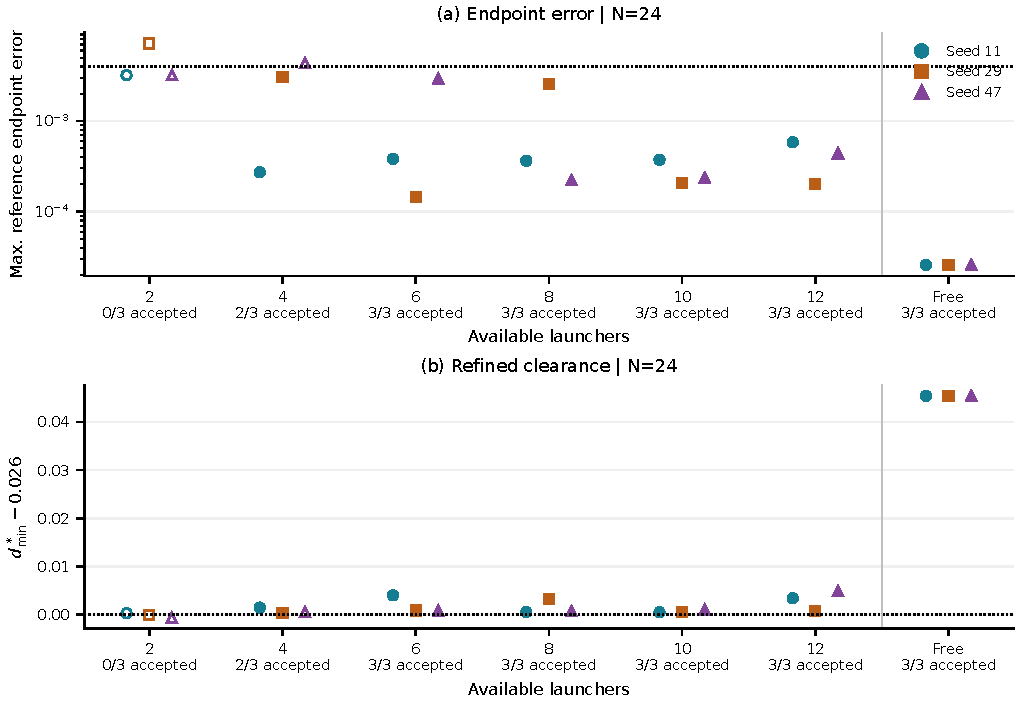
\includegraphics[width=0.95\textwidth]{figs/chapter4/formation-launcher-count.pdf}
% REVIEW-AUDIT Y03 | خطای نهایی و حاشیهٔ فاصله | پذیرش در آرایش‌های دو و چهار ایستگاهی محدود بود. | پیشنهاد: نرخ پذیرش برحسب پیکربندی ایستگاه | مرور؛ نرسیدن به معیار پذیرش | تطبیق با متن گزارش
\caption{\ReviewMark{yellow}{Y03-146-1-1}{خطای نهایی و حاشیهٔ فاصله} برای چیدمان‌های مختلف ایستگاه‌ها.}
\label{fig:results-formation-launcher-count}
\end{figure}

\زیرقسمت{آرایش‌های صدذره‌ای در ناحیه‌های هدف}
\label{sec:results-formation-dense}

چهار ناحیهٔ هدف شامل کپسول، پیکان، ماهی و کپسول دوحفره‌ای بودند.
برای هر ناحیه، همان صد نقطه در سه پیکربندی رهاسازی استفاده شد.
پیکربندی‌ها شامل مکان آزاد و چیدمان‌های شش و دوازده ایستگاهی بودند.
% REVIEW-AUDIT Y05 | برای هر هدف با یک شروع | هشت اجرای ثابت در بودجهٔ آزموده‌شده رد شدند. | پیشنهاد: ردشدن اجراهای ثابت در جست‌وجوی تک‌شروعی | مرور؛ شکست پیکربندی و بودجهٔ محدود | تطبیق با متن گزارش
هر پیکربندی \ReviewMark{yellow}{Y05-156-1-1}{برای هر هدف با یک شروع} ارزیابی شد.
هر چهار برنامهٔ رهاسازی آزاد معیارهای بازپخش را برآورده کردند.
% REVIEW-AUDIT Y05 | ایستگاه‌های ثابت پذیرفته نشدند | هشت اجرای ثابت در بودجهٔ آزموده‌شده رد شدند. | پیشنهاد: ردشدن اجراهای ثابت در جست‌وجوی تک‌شروعی | مرور؛ شکست پیکربندی و بودجهٔ محدود | تطبیق با متن گزارش
هشت اجرای متناظر با \ReviewMark{yellow}{Y05-158-1-1}{ایستگاه‌های ثابت پذیرفته نشدند}.
% REVIEW-AUDIT Y05 | بودجهٔ جست‌وجوی همین آزمون | هشت اجرای ثابت در بودجهٔ آزموده‌شده رد شدند. | پیشنهاد: ردشدن اجراهای ثابت در جست‌وجوی تک‌شروعی | مرور؛ شکست پیکربندی و بودجهٔ محدود | تطبیق با متن گزارش
این نتیجه به چیدمان‌ها و \ReviewMark{yellow}{Y05-159-1-1}{بودجهٔ جست‌وجوی همین آزمون} مربوط است.

شکل~\ref{fig:results-formation-dense} دیسک‌های ذرات را در زمان هدف هر برنامه نشان می‌دهد.
پوشش، نسبت سطح اشغال‌شده در ناحیهٔ هدف به مساحت آن است.
نتایج بازپخش مرجع در جدول~\ref{tab:results-formation-dense} آمده‌اند.
% REVIEW-AUDIT Y06 | بیشترین خطای نهایی و کمترین حاشیهٔ فاصله | ماهی میان نمونه‌های پذیرفته‌شده بدترین حاشیه را دارد. | پیشنهاد: ضعف نسبی ماهی در گروه پذیرفته‌شده | مرور؛ ضعف نسبی در نمونهٔ پذیرفته‌شده | تطبیق با متن گزارش
ماهی \ReviewMark{yellow}{Y06-164-1-1}{بیشترین خطای نهایی و کمترین حاشیهٔ فاصله} را داشت.
% REVIEW-AUDIT Y06 | به مساحت و هندسهٔ ناحیه نیز وابسته است | ماهی میان نمونه‌های پذیرفته‌شده بدترین حاشیه را دارد. | پیشنهاد: ضعف نسبی ماهی در گروه پذیرفته‌شده | مرور؛ ضعف نسبی در نمونهٔ پذیرفته‌شده | تطبیق با متن گزارش
پوشش میان شکل‌ها \ReviewMark{yellow}{Y06-165-1-1}{به مساحت و هندسهٔ ناحیه نیز وابسته است}.

\begin{figure}[htbp]
\centering
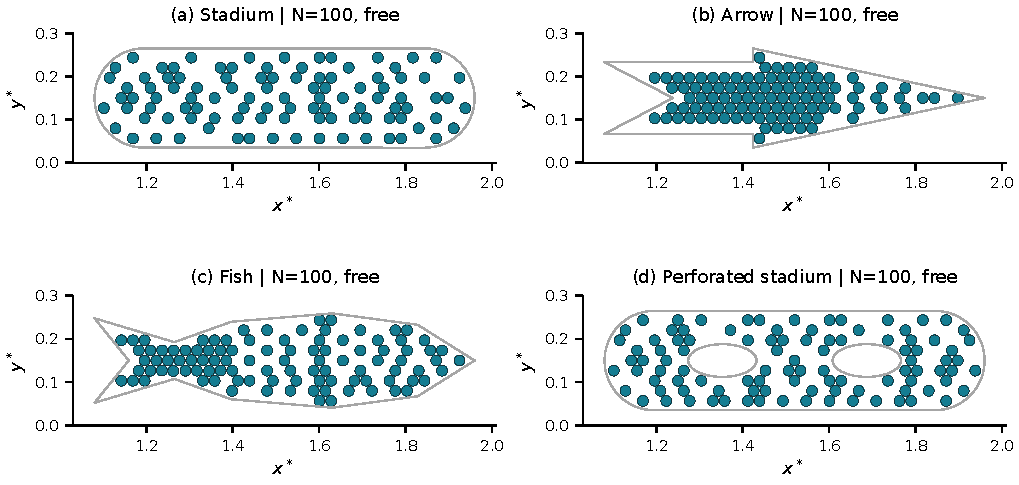
\includegraphics[width=0.95\textwidth]{figs/chapter4/formation-dense-targets.pdf}
\caption{چهار آرایش صدذره‌ای با رهاسازی آزاد در زمان هدف.}
\label{fig:results-formation-dense}
\end{figure}

\begin{table}[htbp]
\centering
\small
\caption{خطا، کمینهٔ فاصله و پوشش چهار آرایش صدذره‌ای پذیرفته‌شده.}
\label{tab:results-formation-dense}
\begin{tabular}{@{}lccc@{}}
\hline
شکل & $E_{\max,\mathrm{ref}}^*$ & $d_{\min,\mathrm{ref}}^*$ & پوشش (\%) \\
\hline
کپسول & $1.21\times10^{-4}$ & $0.026330$ & $25.7$ \\
پیکان & $4.95\times10^{-4}$ & $0.026283$ & $46.5$ \\
ماهی & $1.32\times10^{-3}$ & $0.026197$ & $37.5$ \\
کپسول دوحفره‌ای & $1.21\times10^{-4}$ & $0.026536$ & $28.5$ \\
\hline
\end{tabular}
\end{table}

\زیرقسمت{اثر مکان مرکز آرایش}
\label{sec:results-formation-center}

یک هدف ۱۸ذره‌ای با حفظ هندسه به موقعیت‌های مختلف منتقل شد.
% REVIEW-AUDIT Y07 | ۲۵ برنامه از ۴۹ موقعیت آزموده‌شده پذیرفته شدند | پذیرش مکان هدف با یک شروع سنجیده شد. | پیشنهاد: نرخ پذیرش در پیمایش تک‌شروعی هدف | مرور؛ محدودیت دسترسی و موفقیت جست‌وجو | تطبیق با متن گزارش
با ایستگاه‌های ثابت، \ReviewMark{yellow}{Y07-195-1-1}{۲۵ برنامه از ۴۹ موقعیت آزموده‌شده پذیرفته شدند}.
% REVIEW-AUDIT Y07 | یک شروع بهینه‌سازی | پذیرش مکان هدف با یک شروع سنجیده شد. | پیشنهاد: نرخ پذیرش در پیمایش تک‌شروعی هدف | مرور؛ محدودیت دسترسی و موفقیت جست‌وجو | تطبیق با متن گزارش
برای هر موقعیت، \ReviewMark{yellow}{Y07-196-1-1}{یک شروع بهینه‌سازی} اجرا شد.
% REVIEW-AUDIT Y07 | هیچ‌یک از هفت ارتفاع آزموده‌شده پذیرفته نشد | پذیرش مکان هدف با یک شروع سنجیده شد. | پیشنهاد: نرخ پذیرش در پیمایش تک‌شروعی هدف | مرور؛ محدودیت دسترسی و موفقیت جست‌وجو | تطبیق با متن گزارش
در $x_c^*=0.52$، \ReviewMark{yellow}{Y07-197-1-1}{هیچ‌یک از هفت ارتفاع آزموده‌شده پذیرفته نشد}.
در سه موقعیت طولی انتهایی، هر موقعیت شش پاسخ پذیرفته‌شده داشت.

شکل~\ref{fig:results-formation-center} نقشهٔ حالت ثابت و مقایسهٔ دو روش را نشان می‌دهد.
% REVIEW-AUDIT Y08 | در هفت موقعیت روی خط میانی | خطای بالادست ثابت بی‌بعد است. | پیشنهاد: اختلاف خطای مکانی بی‌بعد در نقطهٔ بالادست | مرور؛ افت عملکرد موضعی | تطبیق با متن گزارش
مقایسهٔ دو روش \ReviewMark{yellow}{Y08-201-1-1}{در هفت موقعیت روی خط میانی} انجام شد.
در خط میانی، شش برنامهٔ ثابت و هفت برنامهٔ آزاد پذیرفته شدند.
% REVIEW-AUDIT Y08 | خطای مرجع حالت ثابت $0.152$ بود | خطای بالادست ثابت بی‌بعد است. | پیشنهاد: اختلاف خطای مکانی بی‌بعد در نقطهٔ بالادست | مرور؛ افت عملکرد موضعی | تطبیق با متن گزارش
در بالادست‌ترین نقطهٔ خط میانی، \ReviewMark{yellow}{Y08-203-1-1}{خطای مرجع حالت ثابت} \ReviewNumber{yellow}{Y08-203-1-2}{$0.152$} \ReviewMark{yellow}{Y08-203-1-3}{بود}.
% REVIEW-AUDIT Y08 | $5.35\times10^{-5}$ | خطای بالادست ثابت بی‌بعد است. | پیشنهاد: اختلاف خطای مکانی بی‌بعد در نقطهٔ بالادست | مرور؛ افت عملکرد موضعی | تطبیق با متن گزارش
خطای مرجع حالت آزاد در همان نقطه حدود \ReviewNumber{yellow}{Y08-204-1-1}{$5.35\times10^{-5}$} بود.

\begin{figure}[htbp]
\centering
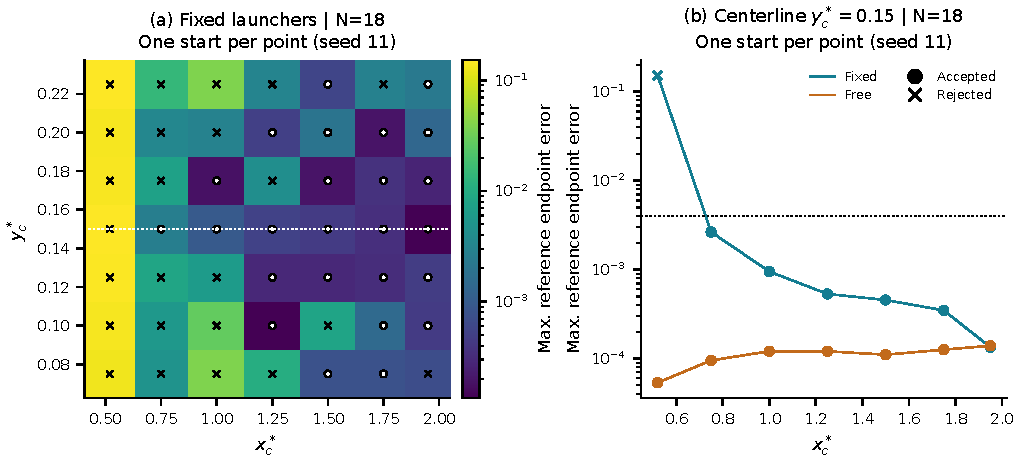
\includegraphics[width=0.95\textwidth]{figs/chapter4/formation-target-center.pdf}
% REVIEW-AUDIT Y07 | اثر مکان مرکز هدف | پذیرش مکان هدف با یک شروع سنجیده شد. | پیشنهاد: نرخ پذیرش در پیمایش تک‌شروعی هدف | مرور؛ محدودیت دسترسی و موفقیت جست‌وجو | تطبیق با متن گزارش
% REVIEW-AUDIT Y08 | مقایسهٔ رهاسازی در خط میانی کانال | خطای بالادست ثابت بی‌بعد است. | پیشنهاد: اختلاف خطای مکانی بی‌بعد در نقطهٔ بالادست | مرور؛ افت عملکرد موضعی | تطبیق با متن گزارش
\caption{\ReviewMark{yellow}{Y07-209-1-1}{اثر مکان مرکز هدف} و \ReviewMark{yellow}{Y08-209-2-1}{مقایسهٔ رهاسازی در خط میانی کانال}.}
\label{fig:results-formation-center}
\end{figure}

\زیرقسمت{اثر زاویه و نسبت محورهای آرایش بیضوی}
\label{sec:results-formation-ellipse}

آرایش ۱۲ذره‌ای برای زاویه‌ها و نسبت محورهای مختلف بررسی شد.
در این پیمایش، مرکز هدف و مساحت بیضی اسمی ثابت بودند.
شکل~\ref{fig:results-formation-ellipse} کوواریانس نقاط هدف و مراکز حاصل را مقایسه می‌کند.
نقشهٔ شکل، میانهٔ خطای کوواریانس شروع‌های انجام‌شده را نشان می‌دهد.
% REVIEW-AUDIT Y09 | از ۵۷ اجرا، ۵۵ اجرا | دو اجرای پیمایش معیارها را برآورده نکردند. | پیشنهاد: پذیرش ۵۵ اجرا از ۵۷ اجرای پیمایش | مرور؛ موفقیت غیرصددرصدی | تطبیق با متن گزارش
\ReviewMark{yellow}{Y09-220-1-1}{از ۵۷ اجرا، ۵۵ اجرا} معیارهای پذیرش را برآورده کردند.

میانهٔ خطای نسبی کوواریانس در اجراهای پذیرفته‌شده حدود $0.076\%$ بود.
بیشینهٔ خطای زاویه برای موارد پذیرفته‌شدهٔ دارای جهت تعریف‌شده، $0.107^\circ$ بود.
% REVIEW-AUDIT Y10 | برای هدف دایره‌ای، جهت محور اصلی تعریف نمی‌شود | محور اصلی دایره جهت یکتا ندارد. | پیشنهاد: جهت محور اصلی برای دایره تعریف‌پذیر نیست | مرور؛ محدودیت تعریف معیار | تطبیق با متن گزارش
\ReviewMark{yellow}{Y10-224-1-1}{برای هدف دایره‌ای، جهت محور اصلی تعریف نمی‌شود}.

\begin{figure}[htbp]
\centering
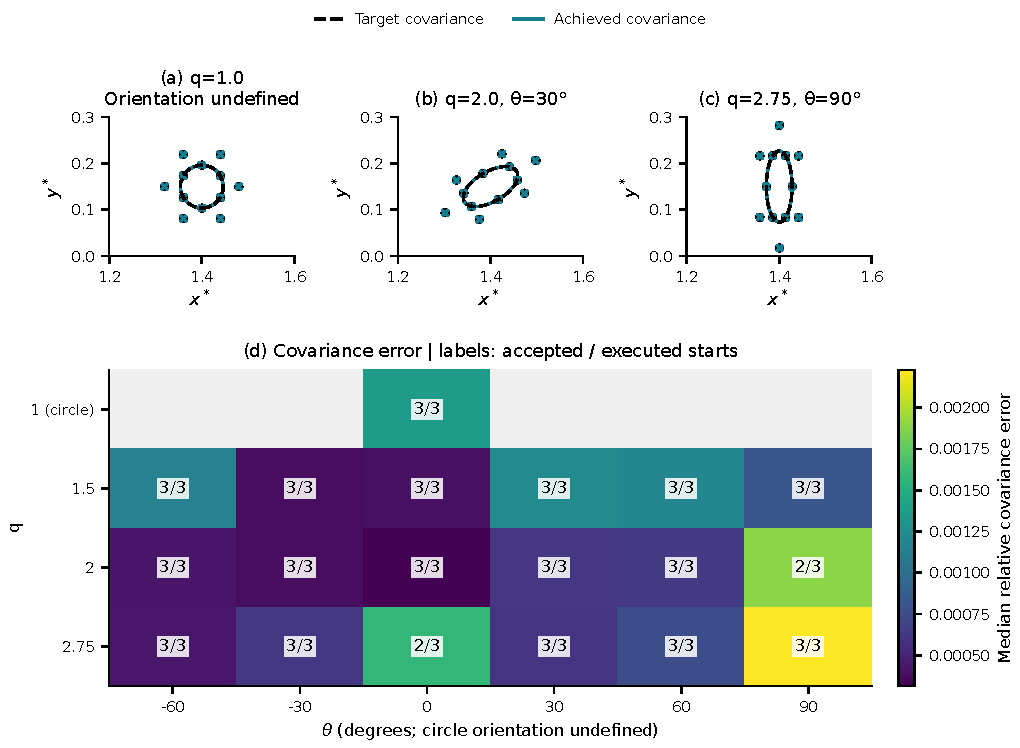
\includegraphics[width=0.95\textwidth]{figs/chapter4/formation-ellipse-covariance.pdf}
% REVIEW-AUDIT Y09 | مقایسهٔ هندسه و کوواریانس | دو اجرای پیمایش معیارها را برآورده نکردند. | پیشنهاد: پذیرش ۵۵ اجرا از ۵۷ اجرای پیمایش | مرور؛ موفقیت غیرصددرصدی | تطبیق با متن گزارش
\caption{\ReviewMark{yellow}{Y09-229-1-1}{مقایسهٔ هندسه و کوواریانس} مراکز هدف و مراکز حاصل.}
\label{fig:results-formation-ellipse}
\end{figure}

\زیرقسمت{کمینهٔ فاصله در طول حرکت و اثر جریمهٔ فاصله}
\label{sec:results-formation-clearance}

شکل~\ref{fig:results-formation-clearance} تغییر فاصلهٔ کمینه را در دو آرایش متراکم نشان می‌دهد.
نمونه‌ها شامل اردک ۴۲ذره‌ای و ماهی ۱۰۰ذره‌ای هستند.
نشانگر جداگانه، کمینهٔ پالایش‌شده را در کنار منحنی نمونه‌برداری‌شده مشخص می‌کند.
کمینهٔ مرجع برای اردک و ماهی به‌ترتیب $0.026048$ و $0.026197$ بود.

در آزمونی جداگانه، اثر جریمهٔ فاصله برای یک آرایش شش‌ذره‌ای بررسی شد.
دو روش با سه شروع متناظر و آزمون پذیرش یکسان مقایسه شدند.
هر سه برنامهٔ دارای جریمه پذیرفته شدند.
% REVIEW-AUDIT Y11 | بدون جریمه به‌دلیل فاصلهٔ ناکافی رد شدند | آزمون حذف جریمه به فاصلهٔ نامقبول انجامید. | پیشنهاد: رد برنامه‌های بدون جریمه در آزمون حذف مؤلفه | مرور؛ آزمون حذف مؤلفه | تطبیق با متن گزارش
هر سه برنامهٔ \ReviewMark{yellow}{Y11-244-1-1}{بدون جریمه به‌دلیل فاصلهٔ ناکافی رد شدند}.
بیشینهٔ خطای نهایی مرجع در هر شش اجرا کمتر از $1.8\times10^{-4}$ بود.
% REVIEW-AUDIT Y11 | ضرورت بررسی فاصلهٔ مراکز در طول حرکت | آزمون حذف جریمه به فاصلهٔ نامقبول انجامید. | پیشنهاد: رد برنامه‌های بدون جریمه در آزمون حذف مؤلفه | مرور؛ آزمون حذف مؤلفه | تطبیق با متن گزارش
این مقایسه \ReviewMark{yellow}{Y11-246-1-1}{ضرورت بررسی فاصلهٔ مراکز در طول حرکت} را نشان می‌دهد.

\begin{figure}[htbp]
\centering
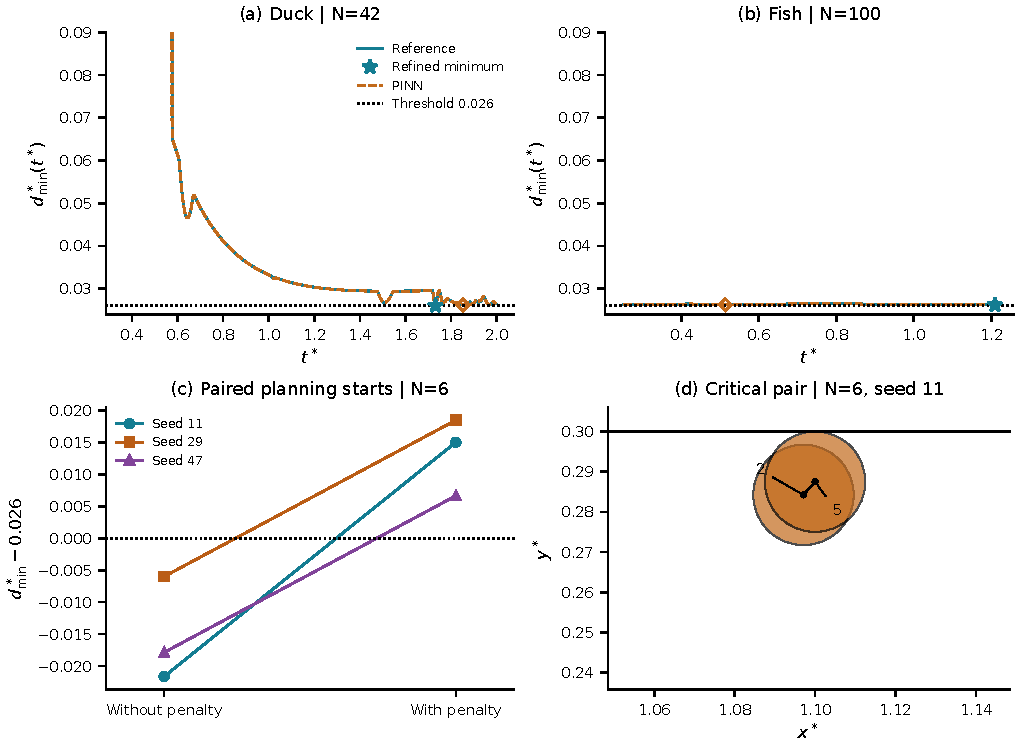
\includegraphics[width=0.95\textwidth]{figs/chapter4/formation-clearance-penalty.pdf}
% REVIEW-AUDIT Y11 | اثر جریمهٔ فاصله | آزمون حذف جریمه به فاصلهٔ نامقبول انجامید. | پیشنهاد: رد برنامه‌های بدون جریمه در آزمون حذف مؤلفه | مرور؛ آزمون حذف مؤلفه | تطبیق با متن گزارش
\caption{کمینهٔ فاصله در آرایش‌های متراکم و \ReviewMark{yellow}{Y11-251-1-1}{اثر جریمهٔ فاصله}.}
\label{fig:results-formation-clearance}
\end{figure}

\clearpage
\قسمت{نتایج پیش‌بینی مستقیم با شبکهٔ عملگر عمیق}
\label{sec:results-forward-deeponet}

در این بخش، پاسخ دو شبکهٔ عملگر عمیق بررسی می‌شود.
شبکهٔ جریان، میدان را برای پروفایل‌های معلوم ورودی پیش‌بینی می‌کند.
شبکهٔ مغناطیسی، مسیر ذره را برای تحریک‌های معلوم پیش‌بینی می‌کند.
وزن‌های هر شبکه در همهٔ مقایسه‌های آن ثابت ماندند.

\زیرقسمت{پیش‌بینی میدان جریان برای پروفایل‌های ورودی متفاوت}
\label{sec:results-forward-flow}

میدان جریان در کانال مستطیلی بی‌بعد با ابعاد $5\times1$ بررسی شد.
مختصات، سرعت و فشار مطابق رابطهٔ~\eqref{eq:forward-flow-scales} بی‌بعد شدند.
چهار ورودی در شکل~\ref{fig:results-forward-flow-inlets} نشان داده شده‌اند.
این ورودی‌ها بتا، تخت، نامتقارن و دارای نه نوسان هستند.
عدد رینولدز هر حالت در شکل و جدول آمده است.

\begin{figure}[htbp]
\centering
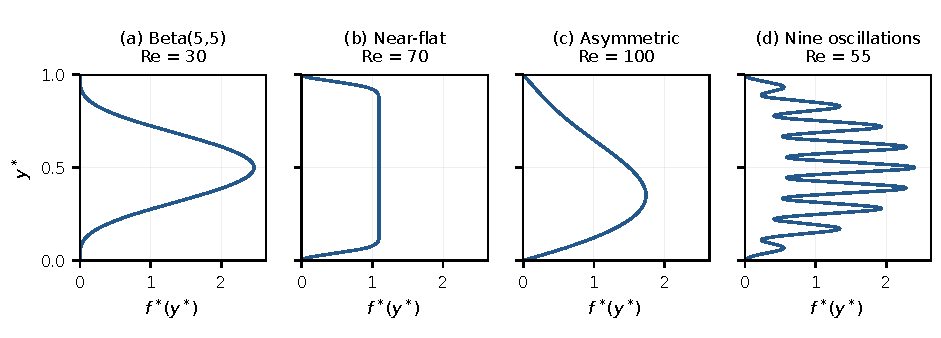
\includegraphics[width=0.95\textwidth]{figs/chapter4/forward-flow-inlets.pdf}
% REVIEW-TERM T18 | ارزیابی تکرارشوندهٔ | ممکن است اجرای چند بذر یا تکرار آماری را القا کند. اگر همان مجموعه در انتخاب وزن استفاده شده، این نقش باید مشخص شود. | پیشنهاد: ارزیابی روی مجموعهٔ مرجعِ انتخاب وزن | پیشنهاد اختیاری؛ رفع ابهام عنوان شکل؛ اطمینان متوسط | ارزیابی چهار مرجع برای انتخاب وزن بود. دو ورودی آزمون نهایی کنار گذاشته شدند. آزمون نهایی اجرا نشده است.؛ مرتبط Y12
% REVIEW-AUDIT Y12 | ارزیابی تکرارشوندهٔ | مجموعهٔ مرجع برای انتخاب وزن به کار رفت. | پیشنهاد: اعتبارسنجیِ انتخاب وزن و آزمون نهایی اجرا‌نشده | مرور؛ محدودیت اعتبارسنجی | ارزیابی چهار مرجع برای انتخاب وزن بود. دو ورودی آزمون نهایی کنار گذاشته شدند. آزمون نهایی اجرا نشده است.؛ مرتبط T18
\caption{پروفایل‌های بی‌بعد ورودی در \ReviewMark{blue}{T18-276-1-1}{ارزیابی تکرارشوندهٔ} عملگر جریان.}
\label{fig:results-forward-flow-inlets}
\end{figure}

مرجع با روش اجزای محدود و شرایط مرزی یکسان محاسبه شد.
شبکه و مرجع در $7081$ نقطهٔ مشترک مقایسه شدند.
تراکم نقاط نزدیک ورودی بیشتر بود.
با ریزترشدن مش، تغییر نسبی سرعت کمتر از $0.010\%$ ماند.
تغییر نسبی فشار در همان بررسی کمتر از $0.20\%$ بود.
فشار با مرجع خروجی مشترک مقایسه شد.
% REVIEW-AUDIT Y12 | حل‌های مرجع در انتخاب وزن نقش داشتند | مجموعهٔ مرجع برای انتخاب وزن به کار رفت. | پیشنهاد: اعتبارسنجیِ انتخاب وزن و آزمون نهایی اجرا‌نشده | مرور؛ محدودیت اعتبارسنجی | ارزیابی چهار مرجع برای انتخاب وزن بود. دو ورودی آزمون نهایی کنار گذاشته شدند. آزمون نهایی اجرا نشده است.
\ReviewMark{yellow}{Y12-286-1-1}{حل‌های مرجع در انتخاب وزن نقش داشتند}.
% REVIEW-AUDIT Y12 | از پاسخ‌های اجزای محدود استفاده نکرد | مجموعهٔ مرجع برای انتخاب وزن به کار رفت. | پیشنهاد: اعتبارسنجیِ انتخاب وزن و آزمون نهایی اجرا‌نشده | مرور؛ محدودیت اعتبارسنجی | ارزیابی چهار مرجع برای انتخاب وزن بود. دو ورودی آزمون نهایی کنار گذاشته شدند. آزمون نهایی اجرا نشده است.
تابع هزینهٔ آموزش \ReviewMark{yellow}{Y12-287-1-1}{از پاسخ‌های اجزای محدود استفاده نکرد}.
% REVIEW-TERM T16 | دو ورودی رزروشده | باید معلوم باشد این نمونه‌ها برای آزمون نهایی کنار گذاشته شده‌اند. نباید به نمونه‌های ارزیابی‌شده تبدیل شوند. | پیشنهاد: دو نمونهٔ ورودیِ کنارگذاشته‌شده برای آزمون نهایی | پیشنهاد اختیاری؛ یکدست‌سازی با T15؛ اطمینان متوسط | ارزیابی چهار مرجع برای انتخاب وزن بود. دو ورودی آزمون نهایی کنار گذاشته شدند. آزمون نهایی اجرا نشده است.؛ مرتبط Y12
% REVIEW-AUDIT Y12 | دو ورودی رزروشده در این ارزیابی بررسی نشدند | مجموعهٔ مرجع برای انتخاب وزن به کار رفت. | پیشنهاد: اعتبارسنجیِ انتخاب وزن و آزمون نهایی اجرا‌نشده | مرور؛ محدودیت اعتبارسنجی | ارزیابی چهار مرجع برای انتخاب وزن بود. دو ورودی آزمون نهایی کنار گذاشته شدند. آزمون نهایی اجرا نشده است.؛ مرتبط T16
\ReviewMark{blue}{T16-288-1-1}{دو ورودی رزروشده} \ReviewMark{yellow}{Y12-288-2-2}{در این ارزیابی بررسی نشدند}.

شکل~\ref{fig:results-forward-flow-beta} میدان ورودی بتا را نشان می‌دهد.
شکل~\ref{fig:results-forward-flow-nine} به ورودی دارای نه نوسان اختصاص دارد.
هر ردیف یک کمیت بی‌بعد را در سه پنل نشان می‌دهد.
پنل‌ها میدان مرجع، پیش‌بینی و اختلاف علامت‌دار را نمایش می‌دهند.
اختلاف از کم‌کردن مرجع از پیش‌بینی به دست می‌آید.
در حالت نوسانی، اختلاف مؤلفهٔ عرضی نزدیک ورودی متمرکزتر است.

\begin{figure}[htbp]
\centering
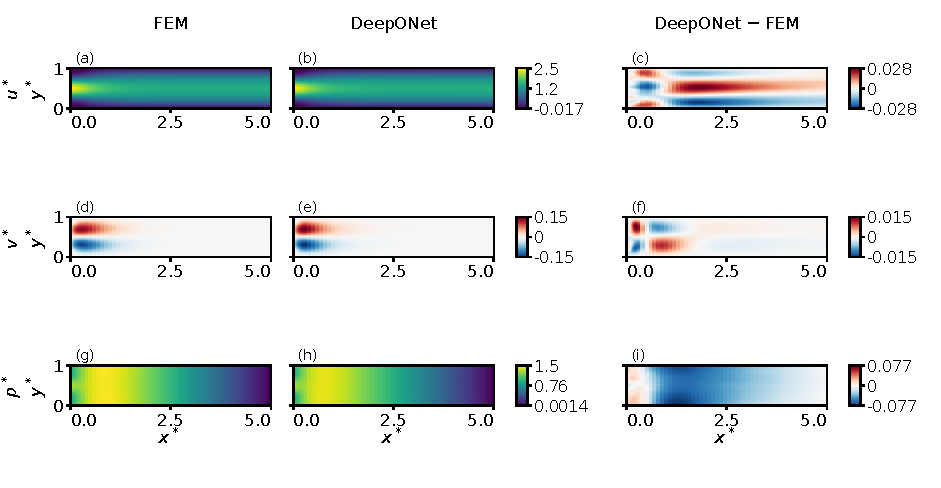
\includegraphics[width=0.98\textwidth,height=0.72\textheight,keepaspectratio]{figs/chapter4/forward-flow-beta.pdf}
\caption{مقایسهٔ میدان پیش‌بینی‌شده و مرجع برای ورودی بتا در $\mathrm{Re}=30$.}
\label{fig:results-forward-flow-beta}
\end{figure}

\begin{figure}[htbp]
\centering
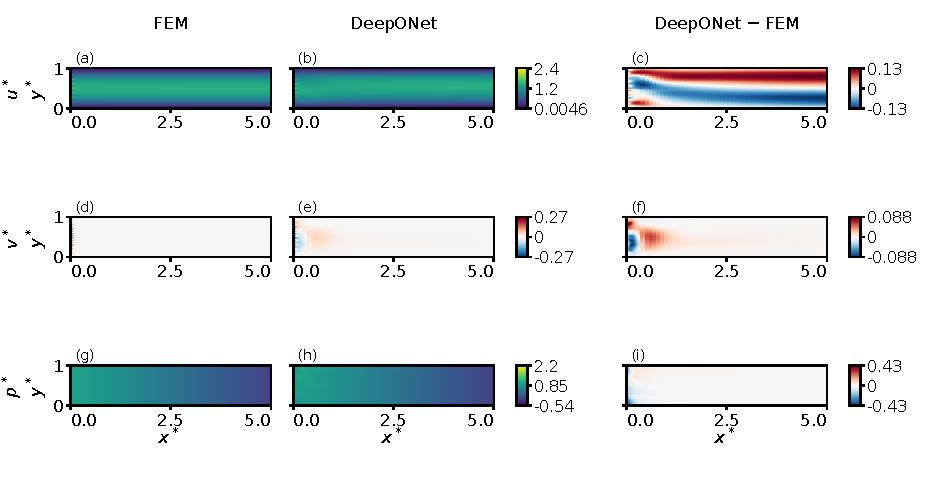
\includegraphics[width=0.98\textwidth,height=0.72\textheight,keepaspectratio]{figs/chapter4/forward-flow-nine.pdf}
% REVIEW-AUDIT Y14 | مقایسهٔ میدان پیش‌بینی‌شده و مرجع برای ورودی نوسانی | خطای نسبی عرضی و خطای بردار دو معیارند. | پیشنهاد: خطای نسبی و RMS مطلق مؤلفهٔ عرضی | بسیار بالا؛ افت دقت مؤلفه‌ای | تطبیق با متن گزارش
\caption{\ReviewMark{yellow}{Y14-307-1-1}{مقایسهٔ میدان پیش‌بینی‌شده و مرجع برای ورودی نوسانی} در $\mathrm{Re}=55$.}
\label{fig:results-forward-flow-nine}
\end{figure}

جدول~\ref{tab:results-forward-flow-errors} خطاهای وزن منتخب را نشان می‌دهد.
این وزن در گام $94000$ ذخیره شد.
خطاهای نسبی مطابق رابطهٔ~\eqref{eq:validation-relative-l2} و برحسب درصد گزارش شده‌اند.
معیارهای ریشهٔ میانگین مربعات مطابق رابطهٔ~\eqref{eq:validation-forward-flow-rms} هستند.

\begin{table}[htbp]
\centering
\small
\setlength{\tabcolsep}{4pt}
% REVIEW-AUDIT Y13 | خطاهای بی‌بعد میدان و باقیماندهٔ مومنتوم | خطاهای عرضی و فشار باید جدا تفسیر شوند. RMS مومنتوم درصد نیست. | پیشنهاد: گزارش تفکیکی خطاهای مؤلفه‌ای و RMS مومنتوم | بسیار بالا؛ خطای زیاد کمّی | تطبیق با متن گزارش
\caption{\ReviewMark{yellow}{Y13-320-1-1}{خطاهای بی‌بعد میدان و باقیماندهٔ مومنتوم} برای وزن منتخب.}
\label{tab:results-forward-flow-errors}
\begin{tabular}{@{}lcccccc@{}}
\hline
ورودی & $\mathrm{Re}$ & $E_2(\mathbf U^*)$ & $E_2(v^*)$ &
$E_{v,\mathrm{rms}}^*$ & $E_2(p^*)$ & $E_{\mathrm{mom,rms}}^*$ \\
\hline
% REVIEW-AUDIT Y13 | $9.261\%$ | خطاهای عرضی و فشار باید جدا تفسیر شوند. RMS مومنتوم درصد نیست. | پیشنهاد: گزارش تفکیکی خطاهای مؤلفه‌ای و RMS مومنتوم | بسیار بالا؛ خطای زیاد کمّی | تطبیق با متن گزارش
% REVIEW-AUDIT Y13 | $0.2759$ | خطاهای عرضی و فشار باید جدا تفسیر شوند. RMS مومنتوم درصد نیست. | پیشنهاد: گزارش تفکیکی خطاهای مؤلفه‌ای و RMS مومنتوم | بسیار بالا؛ خطای زیاد کمّی | تطبیق با متن گزارش
بتا & $30$ & $0.906\%$ & \ReviewNumber{yellow}{Y13-327-1-1}{$9.261\%$} & $0.004159$ & $3.082\%$ & \ReviewNumber{yellow}{Y13-327-2-1}{$0.2759$} \\
% REVIEW-AUDIT Y13 | $39.781\%$ | خطاهای عرضی و فشار باید جدا تفسیر شوند. RMS مومنتوم درصد نیست. | پیشنهاد: گزارش تفکیکی خطاهای مؤلفه‌ای و RMS مومنتوم | بسیار بالا؛ خطای زیاد کمّی | تطبیق با متن گزارش
% REVIEW-AUDIT Y13 | $10.974\%$ | خطاهای عرضی و فشار باید جدا تفسیر شوند. RMS مومنتوم درصد نیست. | پیشنهاد: گزارش تفکیکی خطاهای مؤلفه‌ای و RMS مومنتوم | بسیار بالا؛ خطای زیاد کمّی | تطبیق با متن گزارش
% REVIEW-AUDIT Y13 | $0.5170$ | خطاهای عرضی و فشار باید جدا تفسیر شوند. RMS مومنتوم درصد نیست. | پیشنهاد: گزارش تفکیکی خطاهای مؤلفه‌ای و RMS مومنتوم | بسیار بالا؛ خطای زیاد کمّی | تطبیق با متن گزارش
تخت & $70$ & $3.002\%$ & \ReviewNumber{yellow}{Y13-328-1-1}{$39.781\%$} & $0.010812$ & \ReviewNumber{yellow}{Y13-328-2-1}{$10.974\%$} & \ReviewNumber{yellow}{Y13-328-3-1}{$0.5170$} \\
% REVIEW-AUDIT Y13 | $37.160\%$ | خطاهای عرضی و فشار باید جدا تفسیر شوند. RMS مومنتوم درصد نیست. | پیشنهاد: گزارش تفکیکی خطاهای مؤلفه‌ای و RMS مومنتوم | بسیار بالا؛ خطای زیاد کمّی | تطبیق با متن گزارش
% REVIEW-AUDIT Y13 | $17.845\%$ | خطاهای عرضی و فشار باید جدا تفسیر شوند. RMS مومنتوم درصد نیست. | پیشنهاد: گزارش تفکیکی خطاهای مؤلفه‌ای و RMS مومنتوم | بسیار بالا؛ خطای زیاد کمّی | تطبیق با متن گزارش
% REVIEW-AUDIT Y13 | $0.1509$ | خطاهای عرضی و فشار باید جدا تفسیر شوند. RMS مومنتوم درصد نیست. | پیشنهاد: گزارش تفکیکی خطاهای مؤلفه‌ای و RMS مومنتوم | بسیار بالا؛ خطای زیاد کمّی | تطبیق با متن گزارش
نامتقارن & $100$ & $4.649\%$ & \ReviewNumber{yellow}{Y13-329-1-1}{$37.160\%$} & $0.008145$ & \ReviewNumber{yellow}{Y13-329-2-1}{$17.845\%$} & \ReviewNumber{yellow}{Y13-329-3-1}{$0.1509$} \\
% REVIEW-AUDIT Y13 | $6.604\%$ | خطاهای عرضی و فشار باید جدا تفسیر شوند. RMS مومنتوم درصد نیست. | پیشنهاد: گزارش تفکیکی خطاهای مؤلفه‌ای و RMS مومنتوم | بسیار بالا؛ خطای زیاد کمّی | تطبیق با متن گزارش
% REVIEW-AUDIT Y13 | $89.199\%$ | خطاهای عرضی و فشار باید جدا تفسیر شوند. RMS مومنتوم درصد نیست. | پیشنهاد: گزارش تفکیکی خطاهای مؤلفه‌ای و RMS مومنتوم | بسیار بالا؛ خطای زیاد کمّی | تطبیق با متن گزارش
% REVIEW-AUDIT Y13 | $8.210\%$ | خطاهای عرضی و فشار باید جدا تفسیر شوند. RMS مومنتوم درصد نیست. | پیشنهاد: گزارش تفکیکی خطاهای مؤلفه‌ای و RMS مومنتوم | بسیار بالا؛ خطای زیاد کمّی | تطبیق با متن گزارش
% REVIEW-AUDIT Y13 | $2.0929$ | خطاهای عرضی و فشار باید جدا تفسیر شوند. RMS مومنتوم درصد نیست. | پیشنهاد: گزارش تفکیکی خطاهای مؤلفه‌ای و RMS مومنتوم | بسیار بالا؛ خطای زیاد کمّی | تطبیق با متن گزارش
نه نوسان & $55$ & \ReviewNumber{yellow}{Y13-330-1-1}{$6.604\%$} & \ReviewNumber{yellow}{Y13-330-2-1}{$89.199\%$} & $0.024466$ & \ReviewNumber{yellow}{Y13-330-3-1}{$8.210\%$} & \ReviewNumber{yellow}{Y13-330-4-1}{$2.0929$} \\
\hline
\end{tabular}
\end{table}

ورودی بتا کمترین خطای بردار سرعت و فشار را داشت.
% REVIEW-AUDIT Y14 | خطای نسبی مؤلفهٔ عرضی به $89.199\%$ رسید | خطای نسبی عرضی و خطای بردار دو معیارند. | پیشنهاد: خطای نسبی و RMS مطلق مؤلفهٔ عرضی | بسیار بالا؛ افت دقت مؤلفه‌ای | تطبیق با متن گزارش
در حالت نوسانی، \ReviewMark{yellow}{Y14-336-1-1}{خطای نسبی مؤلفهٔ عرضی به} \ReviewNumber{yellow}{Y14-336-1-2}{$89.199\%$} \ReviewMark{yellow}{Y14-336-1-3}{رسید}.
% REVIEW-AUDIT Y14 | $0.024466$ | خطای نسبی عرضی و خطای بردار دو معیارند. | پیشنهاد: خطای نسبی و RMS مطلق مؤلفهٔ عرضی | بسیار بالا؛ افت دقت مؤلفه‌ای | تطبیق با متن گزارش
ریشهٔ میانگین مربعات همان مؤلفه برابر \ReviewNumber{yellow}{Y14-337-1-1}{$0.024466$} بود.
% REVIEW-AUDIT Y14 | دقت مؤلفهٔ عرضی باید جدا از خطای بردار سرعت سنجیده شود | خطای نسبی عرضی و خطای بردار دو معیارند. | پیشنهاد: خطای نسبی و RMS مطلق مؤلفهٔ عرضی | بسیار بالا؛ افت دقت مؤلفه‌ای | تطبیق با متن گزارش
بنابراین \ReviewMark{yellow}{Y14-338-1-1}{دقت مؤلفهٔ عرضی باید جدا از خطای بردار سرعت سنجیده شود}.
% REVIEW-AUDIT Y14 | بیشترین خطای نسبی فشار در حالت نامتقارن | خطای نسبی عرضی و خطای بردار دو معیارند. | پیشنهاد: خطای نسبی و RMS مطلق مؤلفهٔ عرضی | بسیار بالا؛ افت دقت مؤلفه‌ای | تطبیق با متن گزارش
\ReviewMark{yellow}{Y14-339-1-1}{بیشترین خطای نسبی فشار در حالت نامتقارن} ثبت شد.
% REVIEW-AUDIT Y15 | شکل ورودی و عدد رینولدز هم‌زمان تغییر کردند | شکل ورودی و رینولدز مستقل تغییر نکردند. | پیشنهاد: تغییر هم‌زمان شکل ورودی و عدد رینولدز | بسیار بالا؛ محدودیت نسبت‌دادن علت | تطبیق با متن گزارش
در این مجموعه، \ReviewMark{yellow}{Y15-340-1-1}{شکل ورودی و عدد رینولدز هم‌زمان تغییر کردند}.

% REVIEW-AUDIT Y16 | $5\%$ | سه معیار از هفت معیار برآورده نشدند. | پیشنهاد: معیارهای برآورده‌نشده در ارزیابی وزن منتخب | بسیار بالا؛ رد معیارهای اعلام‌شده | تطبیق با متن گزارش
% REVIEW-AUDIT Y16 | $10\%$ | سه معیار از هفت معیار برآورده نشدند. | پیشنهاد: معیارهای برآورده‌نشده در ارزیابی وزن منتخب | بسیار بالا؛ رد معیارهای اعلام‌شده | تطبیق با متن گزارش
حد پذیرش خطای نسبی سرعت \ReviewNumber{yellow}{Y16-342-1-1}{$5\%$} و فشار \ReviewNumber{yellow}{Y16-342-2-1}{$10\%$} بود.
% REVIEW-AUDIT Y16 | خطای سرعت در حالت نوسانی از حد تعیین‌شده گذشت | سه معیار از هفت معیار برآورده نشدند. | پیشنهاد: معیارهای برآورده‌نشده در ارزیابی وزن منتخب | بسیار بالا؛ رد معیارهای اعلام‌شده | تطبیق با متن گزارش
\ReviewMark{yellow}{Y16-343-1-1}{خطای سرعت در حالت نوسانی از حد تعیین‌شده گذشت}.
% REVIEW-AUDIT Y16 | خطای فشار در حالت‌های تخت و نامتقارن از حد گذشت | سه معیار از هفت معیار برآورده نشدند. | پیشنهاد: معیارهای برآورده‌نشده در ارزیابی وزن منتخب | بسیار بالا؛ رد معیارهای اعلام‌شده | تطبیق با متن گزارش
\ReviewMark{yellow}{Y16-344-1-1}{خطای فشار در حالت‌های تخت و نامتقارن از حد گذشت}.
% REVIEW-AUDIT Y16 | باقیماندهٔ مومنتوم در هر چهار حالت از آستانهٔ $0.05$ بیشتر بود | سه معیار از هفت معیار برآورده نشدند. | پیشنهاد: معیارهای برآورده‌نشده در ارزیابی وزن منتخب | بسیار بالا؛ رد معیارهای اعلام‌شده | تطبیق با متن گزارش
\ReviewMark{yellow}{Y16-345-1-1}{باقیماندهٔ مومنتوم در هر چهار حالت از آستانهٔ} \ReviewNumber{yellow}{Y16-345-1-2}{$0.05$} \ReviewMark{yellow}{Y16-345-1-3}{بیشتر بود}.
معیارهای پیوستگی، شرط خروجی، دبی و خطای ورودی پذیرفته شدند.
% REVIEW-AUDIT Y16 | سه معیار از هفت معیار را برآورده نکرد | سه معیار از هفت معیار برآورده نشدند. | پیشنهاد: معیارهای برآورده‌نشده در ارزیابی وزن منتخب | بسیار بالا؛ رد معیارهای اعلام‌شده | تطبیق با متن گزارش
در مجموع، وزن منتخب \ReviewMark{yellow}{Y16-347-1-1}{سه معیار از هفت معیار را برآورده نکرد}.
% REVIEW-AUDIT Y16 | همان سه معیار را برآورده نکرد | سه معیار از هفت معیار برآورده نشدند. | پیشنهاد: معیارهای برآورده‌نشده در ارزیابی وزن منتخب | بسیار بالا؛ رد معیارهای اعلام‌شده | تطبیق با متن گزارش
وزن گام $100000$ نیز \ReviewMark{yellow}{Y16-348-1-1}{همان سه معیار را برآورده نکرد}.
% REVIEW-AUDIT Y16 | محدودیت میدان در بازسازی معکوس | سه معیار از هفت معیار برآورده نشدند. | پیشنهاد: معیارهای برآورده‌نشده در ارزیابی وزن منتخب | بسیار بالا؛ رد معیارهای اعلام‌شده | تطبیق با متن گزارش
این ارزیابی، مبنای گزارش \ReviewMark{yellow}{Y16-349-1-1}{محدودیت میدان در بازسازی معکوس} است.

با همان وزن، مجموعه‌ای جداگانه از ورودی‌های متنوع نیز بررسی شد.
% REVIEW-AUDIT Y17 | هفت نمونه پس از محاسبهٔ خطای سرعت و فشار انتخاب شدند | انتخاب نمونه‌ها پس از محاسبهٔ خطا انجام شد. | پیشنهاد: مجموعهٔ اکتشافی با انتخاب مبتنی بر خطای مشاهده‌شده | مرور؛ محدودیت تعمیم نمونه‌های خوب | تطبیق با متن گزارش
\ReviewMark{yellow}{Y17-352-1-1}{هفت نمونه پس از محاسبهٔ خطای سرعت و فشار انتخاب شدند}.
در آن‌ها خطای سرعت بین $0.946\%$ و $2.928\%$ بود.
خطای فشار این نمونه‌ها بین $1.833\%$ و $6.839\%$ بود.
این مجموعه نیز یک ورودی با نه دورهٔ نوسان داشت.
% REVIEW-AUDIT Y17 | پوش و دامنهٔ نوسان این ورودی متفاوت بودند | انتخاب نمونه‌ها پس از محاسبهٔ خطا انجام شد. | پیشنهاد: مجموعهٔ اکتشافی با انتخاب مبتنی بر خطای مشاهده‌شده | مرور؛ محدودیت تعمیم نمونه‌های خوب | تطبیق با متن گزارش
در رینولدز $55$، \ReviewMark{yellow}{Y17-356-1-1}{پوش و دامنهٔ نوسان این ورودی متفاوت بودند}.
خطاهای سرعت و فشار آن به‌ترتیب $2.753\%$ و $6.839\%$ بودند.
% REVIEW-AUDIT Y17 | مجموعهٔ اکتشافی | انتخاب نمونه‌ها پس از محاسبهٔ خطا انجام شد. | پیشنهاد: مجموعهٔ اکتشافی با انتخاب مبتنی بر خطای مشاهده‌شده | مرور؛ محدودیت تعمیم نمونه‌های خوب | تطبیق با متن گزارش
این اعداد به ورودی جداگانهٔ \ReviewMark{yellow}{Y17-358-1-1}{مجموعهٔ اکتشافی} تعلق دارند.

\زیرقسمت{پیش‌بینی مسیر ذره تحت تحریک مغناطیسی}
\label{sec:results-forward-magnetic}

عملکرد شبکهٔ \lr{Master10} با دوازده تحریک زمانی بررسی شد.
هندسه، لولهٔ مستقیم با جریان حامل پوازوی بود.
نمای طولی لوله به‌صورت یک ناحیهٔ مستطیلی رسم شده است.
مختصات $X$ و $Z$ به‌ترتیب عرضی و محوری هستند.
این مختصات و زمان $\tau$ مطابق رابطهٔ~\eqref{eq:forward-mag-scales} بی‌بعد شدند.
مقیاس طولی و عرضی به‌ترتیب فاصلهٔ مشخصهٔ منبع و شعاع لوله‌اند.
حل مرجع با روش \lr{DOP853} و معادلهٔ بیش‌میرا محاسبه شد.
مرجع از تابع پیوستهٔ تحریک استفاده کرد.
شبکه در هر پنجره، نمونه‌های زمانی همان تحریک را دریافت کرد.
بیشترین طول پنجرهٔ استنتاج در این مجموعه $0.0125$ بود.

شکل~\ref{fig:results-forward-magnetic-paths} چهار تحریک و پاسخ متناظر را نشان می‌دهد.
بازهٔ نمایش مسیر در هر پنل با دامنهٔ حرکت ذره تنظیم شده است.
پالس گاوسی یک منبع را برای مدتی محدود فعال می‌کند.
در حالت دوم، تحریک از منبع چپ به راست منتقل می‌شود.
در حالت سوم، فرکانس یکی از تحریک‌ها با زمان تغییر می‌کند.
حالت چهارم، تحریک متناوب را با رهاسازی خارج از محور ترکیب می‌کند.
تغییر جهت حرکت عرضی در نمودار $X(\tau)$ دیده می‌شود.

\begin{figure}[htbp]
\centering
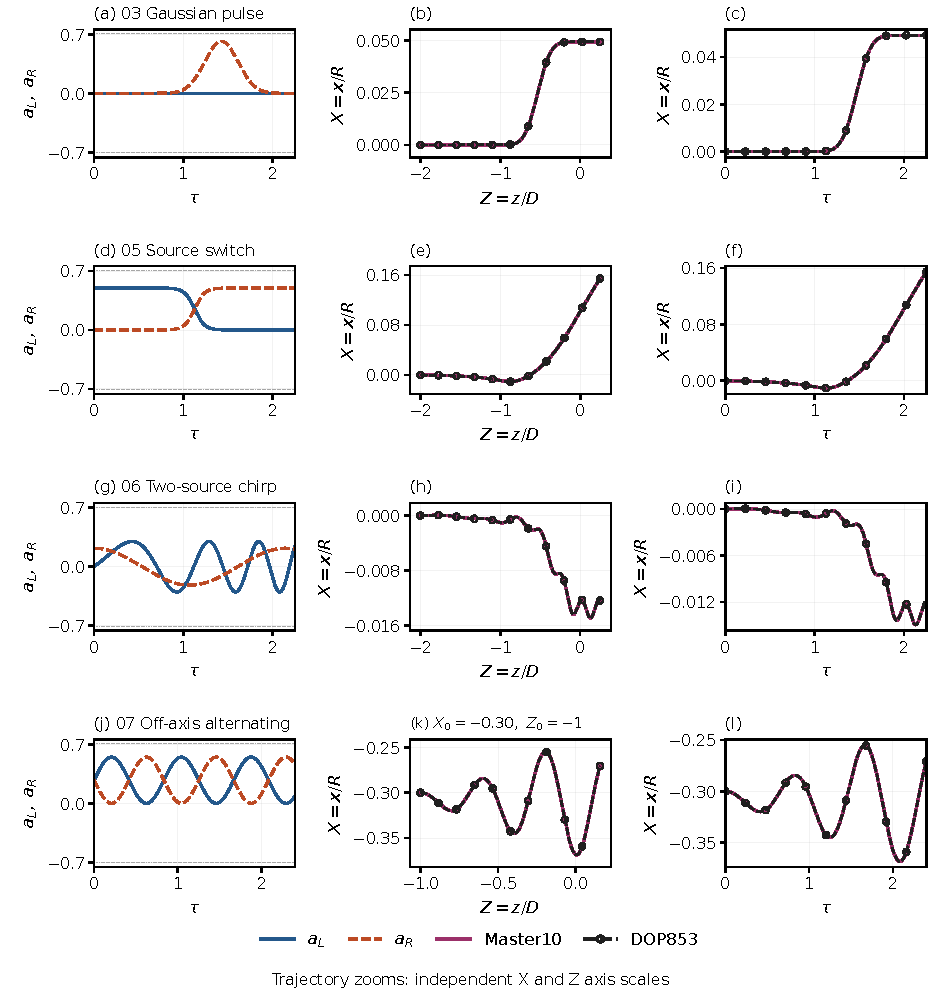
\includegraphics[width=0.98\textwidth,height=0.78\textheight,keepaspectratio]{figs/chapter4/forward-magnetic-paths.pdf}
\caption{تحریک منابع، مسیر فضایی و پاسخ عرضی در چهار نمونه.}
\label{fig:results-forward-magnetic-paths}
\end{figure}

مسیرهای شبکه و مرجع روی $801$ زمان مشترک مقایسه شدند.
بیشینهٔ خطاهای عرضی و محوری مطابق رابطهٔ~\eqref{eq:validation-forward-magnetic-errors} محاسبه شدند.
جدول~\ref{tab:results-forward-magnetic-errors} بیشینهٔ خطاها را برای هر دوازده حالت نشان می‌دهد.
حد پذیرش عرضی $10^{-2}$ و حد محوری $3.75\times10^{-4}$ بود.
هر دوازده حالت از نظر هر دو مؤلفه پذیرفته شدند.
حساسیت مرجع به نصف‌شدن گام بیشینه نیز بررسی شد.
این گام از $1.5\times10^{-3}$ به $7.5\times10^{-4}$ کاهش یافت.
پاسخ بدون میدان نیز با جواب تحلیلی مقایسه شد.

\begin{table}[htbp]
\centering
\small
\setlength{\tabcolsep}{4pt}
\renewcommand{\arraystretch}{0.85}
\caption{شرایط آغاز و بیشینهٔ خطاهای بی‌بعد مسیر برای دوازده تحریک.}
\label{tab:results-forward-magnetic-errors}
\begin{tabular}{@{}llccccc@{}}
\hline
شناسه & تحریک & $X_0$ & $Z_0$ & $\tau_f$ &
$10^5 E_{X,\infty}$ & $10^5 E_{Z,\infty}$ \\
\hline
$01$ & ثابت راست & $0$ & $-2$ & $2.25$ & $5.017$ & $1.532$ \\
$02$ & ثابت چپ & $0$ & $-2$ & $2.25$ & $0.785$ & $1.161$ \\
$03$ & پالس گاوسی & $0$ & $-2$ & $2.25$ & $3.199$ & $0.208$ \\
$04$ & سینوسی & $0$ & $-2$ & $2.25$ & $5.349$ & $0.700$ \\
$05$ & تغییر منبع & $0$ & $-2$ & $2.25$ & $2.618$ & $1.212$ \\
$06$ & فرکانس متغیر & $0$ & $-2$ & $2.25$ & $2.035$ & $0.789$ \\
$07$ & تحریک متناوب خارج از محور & $-0.30$ & $-1$ & $2.40$ & $5.066$ & $3.257$ \\
$08$ & پالس‌های متناوب & $0.35$ & $-1.125$ & $2.10$ & $1.885$ & $1.192$ \\
$09$ & فرکانس متغیر دو منبع & $0.15$ & $-0.625$ & $2.25$ & $4.460$ & $0.608$ \\
$10$ & تحریک چندفرکانسی & $-0.40$ & $-1.875$ & $1.35$ & $2.358$ & $3.243$ \\
$11$ & تغییر منبع در پایین‌دست & $0.25$ & $0.50$ & $1.50$ & $2.286$ & $0.550$ \\
$12$ & تحریک با اختلاف فاز & $-0.25$ & $-1.50$ & $2.40$ & $0.957$ & $1.352$ \\
\hline
\end{tabular}
\end{table}

بزرگ‌ترین خطای عرضی، $5.349\times10^{-5}$، در حالت سینوسی ثبت شد.
بزرگ‌ترین خطای محوری، $3.257\times10^{-5}$، به رهاسازی خارج از محور تعلق داشت.
شکل~\ref{fig:results-forward-magnetic-errors} تغییر خطای دو مؤلفه را در زمان نشان می‌دهد.
در این نمودارها، خطای مطلق بر مقیاس ثابت هر مختصات تقسیم شد.
به‌این‌ترتیب، عبور از مبدأ باعث قلهٔ مصنوعی در خطا نمی‌شود.

\begin{figure}[htbp]
\centering
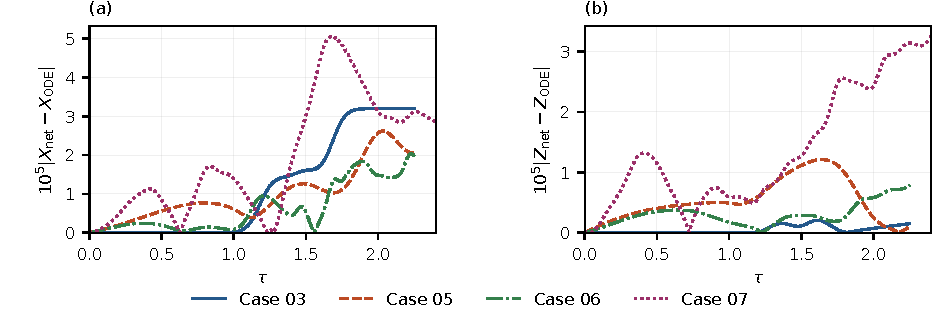
\includegraphics[width=0.94\textwidth]{figs/chapter4/forward-magnetic-errors.pdf}
\caption{تغییر زمانی خطای مطلق بی‌بعد مسیر در دو راستای عرضی و محوری.}
\label{fig:results-forward-magnetic-errors}
\end{figure}

% REVIEW-AUDIT Y18 | اثر نمونه‌برداری، تقریب شبکه و اتصال پنجره‌ها | اعتبار مقایسه به مدل بیش‌میرا و فرض‌های آن محدود است. | پیشنهاد: دامنهٔ اعتبار مدل بیش‌میرا با دو منبع ثابت | مرور؛ دامنهٔ اعتبار فیزیکی | تطبیق با متن گزارش
خطای گزارش‌شده، \ReviewMark{yellow}{Y18-439-1-1}{اثر نمونه‌برداری، تقریب شبکه و اتصال پنجره‌ها} را شامل می‌شود.
% REVIEW-AUDIT Y18 | معادلهٔ بیش‌میرا و دو منبع ثابت | اعتبار مقایسه به مدل بیش‌میرا و فرض‌های آن محدود است. | پیشنهاد: دامنهٔ اعتبار مدل بیش‌میرا با دو منبع ثابت | مرور؛ دامنهٔ اعتبار فیزیکی | تطبیق با متن گزارش
این مقایسه به \ReviewMark{yellow}{Y18-440-1-1}{معادلهٔ بیش‌میرا و دو منبع ثابت} مربوط است.
% REVIEW-AUDIT Y18 | حرکت براونی، گرانش و گذرای اینرسی در هر دو پاسخ حذف شدند | اعتبار مقایسه به مدل بیش‌میرا و فرض‌های آن محدود است. | پیشنهاد: دامنهٔ اعتبار مدل بیش‌میرا با دو منبع ثابت | مرور؛ دامنهٔ اعتبار فیزیکی | تطبیق با متن گزارش
\ReviewMark{yellow}{Y18-441-1-1}{حرکت براونی، گرانش و گذرای اینرسی در هر دو پاسخ حذف شدند}.
% REVIEW-AUDIT Y18 | دامنهٔ تحریک در حالت‌های بررسی‌شده از قید بخش | اعتبار مقایسه به مدل بیش‌میرا و فرض‌های آن محدود است. | پیشنهاد: دامنهٔ اعتبار مدل بیش‌میرا با دو منبع ثابت | مرور؛ دامنهٔ اعتبار فیزیکی | تطبیق با متن گزارش
\ReviewMark{yellow}{Y18-442-1-1}{دامنهٔ تحریک در حالت‌های بررسی‌شده از قید بخش}~\ref{sec:forward-magnetic-operator} پیروی کرد.

\clearpage
\قسمت{نتایج بازسازی معکوس و رهگیری مسیر}
\label{sec:results-inverse-and-tracking}

ابتدا بازسازی جریان از دو مسیر ذره بررسی می‌شود.
سپس دو روش با زمان و بدون زمان مقایسه می‌شوند.
نتایج رهگیری مغناطیسی به مدل نهم تعلق دارند.

\زیرقسمت{بازسازی جریان از دو مسیر زمان‌دار}
\label{sec:results-inverse-flow-timed}

% REVIEW-AUDIT Y19 | کانال مستطیلی بی‌بعد | آزمون از مسیر مصنوعی و شرایط اولیهٔ معلوم استفاده کرد. | پیشنهاد: بازسازی مصنوعی با اطلاعات اولیهٔ معلوم | مرور؛ فرض‌ها و دامنهٔ آزمایش | الف corners_beta5 و ب corners_beta4 است. هر دو از گوشه‌های بالاچپ و پایین‌راست شروع می‌کنند.
بازسازی در \ReviewMark{yellow}{Y19-455-1-1}{کانال مستطیلی بی‌بعد} با ابعاد $5\times1$ انجام شد.
% REVIEW-AUDIT Y19 | مسیرهای مصنوعی از جریان مرجع اجزای محدود | آزمون از مسیر مصنوعی و شرایط اولیهٔ معلوم استفاده کرد. | پیشنهاد: بازسازی مصنوعی با اطلاعات اولیهٔ معلوم | مرور؛ فرض‌ها و دامنهٔ آزمایش | الف corners_beta5 و ب corners_beta4 است. هر دو از گوشه‌های بالاچپ و پایین‌راست شروع می‌کنند.
\ReviewMark{yellow}{Y19-456-1-1}{مسیرهای مصنوعی از جریان مرجع اجزای محدود} به دست آمدند.
% REVIEW-AUDIT Y19 | عدد رینولدز مرجع در هر سه نمونه | آزمون از مسیر مصنوعی و شرایط اولیهٔ معلوم استفاده کرد. | پیشنهاد: بازسازی مصنوعی با اطلاعات اولیهٔ معلوم | مرور؛ فرض‌ها و دامنهٔ آزمایش | الف corners_beta5 و ب corners_beta4 است. هر دو از گوشه‌های بالاچپ و پایین‌راست شروع می‌کنند.
\ReviewMark{yellow}{Y19-457-1-1}{عدد رینولدز مرجع در هر سه نمونه} $30$ بود.
% REVIEW-AUDIT Y19 | سرعت‌های اولیه و اعداد استوکس در هر نمونه معلوم بودند | آزمون از مسیر مصنوعی و شرایط اولیهٔ معلوم استفاده کرد. | پیشنهاد: بازسازی مصنوعی با اطلاعات اولیهٔ معلوم | مرور؛ فرض‌ها و دامنهٔ آزمایش | الف corners_beta5 و ب corners_beta4 است. هر دو از گوشه‌های بالاچپ و پایین‌راست شروع می‌کنند.
\ReviewMark{yellow}{Y19-458-1-1}{سرعت‌های اولیه و اعداد استوکس در هر نمونه معلوم بودند}.
% REVIEW-AUDIT Y19 | $2\times10^{-4}$ | آزمون از مسیر مصنوعی و شرایط اولیهٔ معلوم استفاده کرد. | پیشنهاد: بازسازی مصنوعی با اطلاعات اولیهٔ معلوم | مرور؛ فرض‌ها و دامنهٔ آزمایش | الف corners_beta5 و ب corners_beta4 است. هر دو از گوشه‌های بالاچپ و پایین‌راست شروع می‌کنند.
به موقعیت‌ها نویزی با انحراف معیار بی‌بعد \ReviewNumber{yellow}{Y19-459-1-1}{$2\times10^{-4}$} افزوده شد.
% REVIEW-AUDIT Y19 | موقعیت اولیهٔ هر ذره بدون اغتشاش باقی ماند | آزمون از مسیر مصنوعی و شرایط اولیهٔ معلوم استفاده کرد. | پیشنهاد: بازسازی مصنوعی با اطلاعات اولیهٔ معلوم | مرور؛ فرض‌ها و دامنهٔ آزمایش | الف corners_beta5 و ب corners_beta4 است. هر دو از گوشه‌های بالاچپ و پایین‌راست شروع می‌کنند.
\ReviewMark{yellow}{Y19-460-1-1}{موقعیت اولیهٔ هر ذره بدون اغتشاش باقی ماند}.
پروفایل و میدان مرجع فقط برای ارزیابی پس از برازش استفاده شدند.
در هر سه بازسازی، وزن‌های گام $94000$ ثابت ماندند.

مختصات مکان با ارتفاع کانال مقیاس شدند.
مقیاس زمان $H/U_{\mathrm{ref}}$ است.
پروفایل و میدان با مقیاس مشترک بخش~\ref{sec:inverse-flow-timed} مقایسه شدند.
سرعت میانگین تخمینی با $A=\bar U/U_{\mathrm{ref}}$ گزارش می‌شود.

% REVIEW-TERM T19 | نمونهٔ گوشه‌ای الف | در متن، تعریف کافی برای گوشه‌ای دیده نمی‌شود. corner case الزاماً به ذرات نزدیک گوشهٔ کانال اشاره ندارد. نام اصلی و تنظیمات نمونه باید بررسی شوند. | پیشنهاد: سناریوی رهاسازی از دو گوشهٔ مقابل، با شناسهٔ الف یا ب | شناسهٔ نامفهوم؛ نیازمند بررسی منبع | الف corners_beta5 و ب corners_beta4 است. هر دو از گوشه‌های بالاچپ و پایین‌راست شروع می‌کنند.
شکل~\ref{fig:results-inverse-timed-replay} بازپخش \ReviewMark{blue}{T19-469-1-1}{نمونهٔ گوشه‌ای الف} را نشان می‌دهد.
در بازپخش، معادلهٔ حرکت از شرایط اولیه دوباره انتگرال‌گیری شد.
سرعت سیال در مکان جاری ذره خوانده شد.
خطای مکانی در زمان‌های مشاهده محاسبه شد.
پروفایل ورودی تخمینی نیز با پروفایل مرجع مقایسه شده است.

\begin{figure}[htbp]
\centering
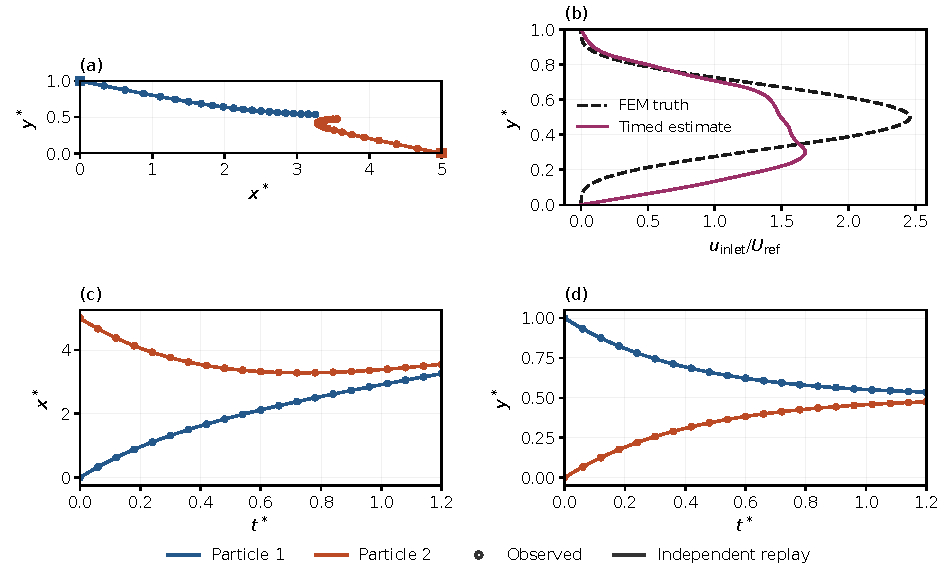
\includegraphics[width=0.97\textwidth,height=0.68\textheight,keepaspectratio]{figs/chapter4/inverse-timed-replay.pdf}
% REVIEW-TERM T19 | نمونهٔ گوشه‌ای الف | در متن، تعریف کافی برای گوشه‌ای دیده نمی‌شود. corner case الزاماً به ذرات نزدیک گوشهٔ کانال اشاره ندارد. نام اصلی و تنظیمات نمونه باید بررسی شوند. | پیشنهاد: سناریوی رهاسازی از دو گوشهٔ مقابل، با شناسهٔ الف یا ب | شناسهٔ نامفهوم؛ نیازمند بررسی منبع | الف corners_beta5 و ب corners_beta4 است. هر دو از گوشه‌های بالاچپ و پایین‌راست شروع می‌کنند.
\caption{مقایسهٔ مسیرها و پروفایل ورودی در بازسازی زمان‌دار \ReviewMark{blue}{T19-478-1-1}{نمونهٔ گوشه‌ای الف}.}
\label{fig:results-inverse-timed-replay}
\end{figure}

شکل~\ref{fig:results-inverse-timed-fields} سه مؤلفهٔ میدان همان نمونه را نشان می‌دهد.
% REVIEW-AUDIT Y20 | اختلاف علامت‌دار | اختلاف میدان در خارج از مسیرها نیز دیده می‌شود. | پیشنهاد: اختلاف علامت‌دار میدان در نواحی دور از مسیر | مرور؛ ضعف بازسازی خارج از مسیر | تطبیق با متن گزارش
هر ردیف شامل میدان مرجع، میدان تخمینی و \ReviewMark{yellow}{Y20-483-1-1}{اختلاف علامت‌دار} است.
اختلاف از کم‌کردن مرجع از تخمین به دست می‌آید.
% REVIEW-AUDIT Y20 | دور از مسیرها نیز دیده می‌شود | اختلاف میدان در خارج از مسیرها نیز دیده می‌شود. | پیشنهاد: اختلاف علامت‌دار میدان در نواحی دور از مسیر | مرور؛ ضعف بازسازی خارج از مسیر | تطبیق با متن گزارش
اختلاف در بخش‌هایی از کانال، \ReviewMark{yellow}{Y20-485-1-1}{دور از مسیرها نیز دیده می‌شود}.

\begin{figure}[htbp]
\centering
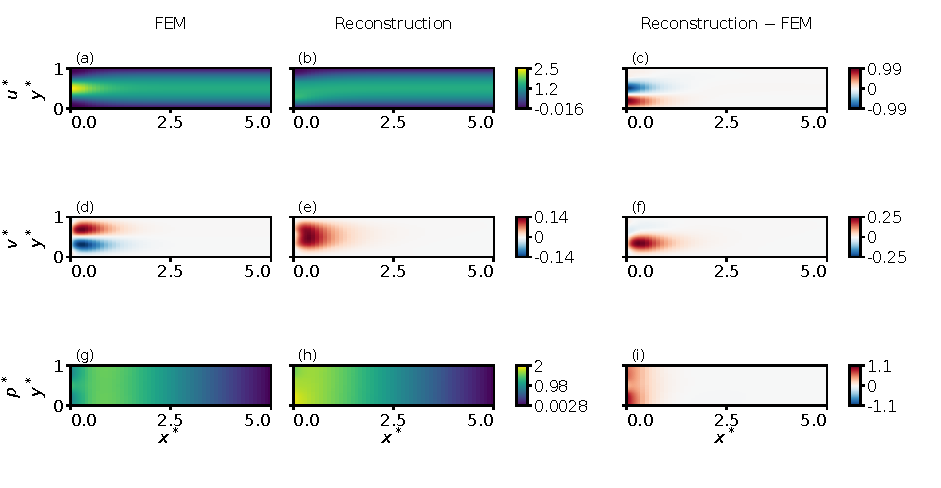
\includegraphics[width=0.98\textwidth,height=0.72\textheight,keepaspectratio]{figs/chapter4/inverse-timed-fields.pdf}
% REVIEW-TERM T19 | نمونهٔ گوشه‌ای الف | در متن، تعریف کافی برای گوشه‌ای دیده نمی‌شود. corner case الزاماً به ذرات نزدیک گوشهٔ کانال اشاره ندارد. نام اصلی و تنظیمات نمونه باید بررسی شوند. | پیشنهاد: سناریوی رهاسازی از دو گوشهٔ مقابل، با شناسهٔ الف یا ب | شناسهٔ نامفهوم؛ نیازمند بررسی منبع | الف corners_beta5 و ب corners_beta4 است. هر دو از گوشه‌های بالاچپ و پایین‌راست شروع می‌کنند.؛ مرتبط Y20
% REVIEW-AUDIT Y20 | مقایسهٔ میدان بازسازی‌شده و مرجع اجزای محدود | اختلاف میدان در خارج از مسیرها نیز دیده می‌شود. | پیشنهاد: اختلاف علامت‌دار میدان در نواحی دور از مسیر | مرور؛ ضعف بازسازی خارج از مسیر | تطبیق با متن گزارش؛ مرتبط T19
\caption{\ReviewMark{yellow}{Y20-490-2-1}{مقایسهٔ میدان بازسازی‌شده و مرجع اجزای محدود} در \ReviewMark{blue}{T19-490-1-1}{نمونهٔ گوشه‌ای الف}.}
\label{fig:results-inverse-timed-fields}
\end{figure}

جدول~\ref{tab:results-inverse-timed} خطاهای مسیر، پروفایل و میدان را گزارش می‌کند.
معیار مسیر از رابطهٔ~\eqref{eq:validation-inverse-timed-path} به دست می‌آید.
خطاهای نسبی میدان مطابق رابطهٔ~\eqref{eq:validation-relative-l2} محاسبه شدند.
هر شش بازپخش به پایان بازهٔ مشاهده رسیدند.
% REVIEW-AUDIT Y21 | با رسیدن به سقف تکرار پایان یافت | سقف تکرار علت توقف شروع‌های منتخب بود. | پیشنهاد: پایان بهینه‌سازی در سقف تکرار | مرور؛ همگرایی تأییدنشده | تطبیق با متن گزارش
بهینه‌سازی در شروع‌های منتخب \ReviewMark{yellow}{Y21-498-1-1}{با رسیدن به سقف تکرار پایان یافت}.

\begin{table}[htbp]
\centering
\small
\setlength{\tabcolsep}{4pt}
% REVIEW-AUDIT Y22 | مقایسهٔ بازسازی زمان‌دار با مرجع | خطای موقعیت مسیر با خطای بازسازی میدان تفاوت دارد. | پیشنهاد: خطاهای جداگانهٔ ورودی، سرعت و فشار | بسیار بالا؛ خطای زیاد مجهول و میدان | تطبیق با متن گزارش
\caption{خطاهای بی‌بعد بازپخش و \ReviewMark{yellow}{Y22-504-1-1}{مقایسهٔ بازسازی زمان‌دار با مرجع}.}
\label{tab:results-inverse-timed}
\begin{tabular}{@{}lcccccc@{}}
\hline
نمونه & $10^4 E_{1,\mathrm{rms}}^*$ & $10^4 E_{2,\mathrm{rms}}^*$ & $A$ &
$E_2(f_{\mathrm{ref}}^*)$ & $E_2(\mathbf U_{\mathrm{ref}}^*)$ & $E_2(p_{\mathrm{ref}}^*)$ \\
\hline
% REVIEW-TERM T19 | گوشه‌ای ب | در متن، تعریف کافی برای گوشه‌ای دیده نمی‌شود. corner case الزاماً به ذرات نزدیک گوشهٔ کانال اشاره ندارد. نام اصلی و تنظیمات نمونه باید بررسی شوند. | پیشنهاد: سناریوی رهاسازی از دو گوشهٔ مقابل، با شناسهٔ الف یا ب | شناسهٔ نامفهوم؛ نیازمند بررسی منبع | الف corners_beta5 و ب corners_beta4 است. هر دو از گوشه‌های بالاچپ و پایین‌راست شروع می‌کنند.؛ مرتبط Y22
% REVIEW-AUDIT Y22 | $32.423\%$ | خطای موقعیت مسیر با خطای بازسازی میدان تفاوت دارد. | پیشنهاد: خطاهای جداگانهٔ ورودی، سرعت و فشار | بسیار بالا؛ خطای زیاد مجهول و میدان | تطبیق با متن گزارش؛ مرتبط T19
% REVIEW-AUDIT Y22 | $19.505\%$ | خطای موقعیت مسیر با خطای بازسازی میدان تفاوت دارد. | پیشنهاد: خطاهای جداگانهٔ ورودی، سرعت و فشار | بسیار بالا؛ خطای زیاد مجهول و میدان | تطبیق با متن گزارش؛ مرتبط T19
% REVIEW-AUDIT Y22 | $20.795\%$ | خطای موقعیت مسیر با خطای بازسازی میدان تفاوت دارد. | پیشنهاد: خطاهای جداگانهٔ ورودی، سرعت و فشار | بسیار بالا؛ خطای زیاد مجهول و میدان | تطبیق با متن گزارش؛ مرتبط T19
\ReviewMark{blue}{T19-511-1-1}{گوشه‌ای ب} & $4.443$ & $3.768$ & $1.00194$ & \ReviewNumber{yellow}{Y22-511-2-1}{$32.423\%$} & \ReviewNumber{yellow}{Y22-511-3-1}{$19.505\%$} & \ReviewNumber{yellow}{Y22-511-4-1}{$20.795\%$} \\
% REVIEW-TERM T19 | گوشه‌ای الف | در متن، تعریف کافی برای گوشه‌ای دیده نمی‌شود. corner case الزاماً به ذرات نزدیک گوشهٔ کانال اشاره ندارد. نام اصلی و تنظیمات نمونه باید بررسی شوند. | پیشنهاد: سناریوی رهاسازی از دو گوشهٔ مقابل، با شناسهٔ الف یا ب | شناسهٔ نامفهوم؛ نیازمند بررسی منبع | الف corners_beta5 و ب corners_beta4 است. هر دو از گوشه‌های بالاچپ و پایین‌راست شروع می‌کنند.؛ مرتبط Y22
% REVIEW-AUDIT Y22 | $43.153\%$ | خطای موقعیت مسیر با خطای بازسازی میدان تفاوت دارد. | پیشنهاد: خطاهای جداگانهٔ ورودی، سرعت و فشار | بسیار بالا؛ خطای زیاد مجهول و میدان | تطبیق با متن گزارش؛ مرتبط T19
% REVIEW-AUDIT Y22 | $26.913\%$ | خطای موقعیت مسیر با خطای بازسازی میدان تفاوت دارد. | پیشنهاد: خطاهای جداگانهٔ ورودی، سرعت و فشار | بسیار بالا؛ خطای زیاد مجهول و میدان | تطبیق با متن گزارش؛ مرتبط T19
% REVIEW-AUDIT Y22 | $32.999\%$ | خطای موقعیت مسیر با خطای بازسازی میدان تفاوت دارد. | پیشنهاد: خطاهای جداگانهٔ ورودی، سرعت و فشار | بسیار بالا؛ خطای زیاد مجهول و میدان | تطبیق با متن گزارش؛ مرتبط T19
\ReviewMark{blue}{T19-512-1-1}{گوشه‌ای الف} & $6.676$ & $4.821$ & $1.00236$ & \ReviewNumber{yellow}{Y22-512-2-1}{$43.153\%$} & \ReviewNumber{yellow}{Y22-512-3-1}{$26.913\%$} & \ReviewNumber{yellow}{Y22-512-4-1}{$32.999\%$} \\
% REVIEW-AUDIT Y22 | $40.213\%$ | خطای موقعیت مسیر با خطای بازسازی میدان تفاوت دارد. | پیشنهاد: خطاهای جداگانهٔ ورودی، سرعت و فشار | بسیار بالا؛ خطای زیاد مجهول و میدان | تطبیق با متن گزارش
% REVIEW-AUDIT Y22 | $21.217\%$ | خطای موقعیت مسیر با خطای بازسازی میدان تفاوت دارد. | پیشنهاد: خطاهای جداگانهٔ ورودی، سرعت و فشار | بسیار بالا؛ خطای زیاد مجهول و میدان | تطبیق با متن گزارش
% REVIEW-AUDIT Y22 | $42.804\%$ | خطای موقعیت مسیر با خطای بازسازی میدان تفاوت دارد. | پیشنهاد: خطاهای جداگانهٔ ورودی، سرعت و فشار | بسیار بالا؛ خطای زیاد مجهول و میدان | تطبیق با متن گزارش
مایل & $18.984$ & $10.001$ & $1.01047$ & \ReviewNumber{yellow}{Y22-513-1-1}{$40.213\%$} & \ReviewNumber{yellow}{Y22-513-2-1}{$21.217\%$} & \ReviewNumber{yellow}{Y22-513-3-1}{$42.804\%$} \\
\hline
\end{tabular}
\end{table}

در جدول، $f_{\mathrm{ref}}^*$ پروفایل ورودی در مقیاس سرعت مرجع است.
% REVIEW-TERM T19 | نمونهٔ گوشه‌ای الف | در متن، تعریف کافی برای گوشه‌ای دیده نمی‌شود. corner case الزاماً به ذرات نزدیک گوشهٔ کانال اشاره ندارد. نام اصلی و تنظیمات نمونه باید بررسی شوند. | پیشنهاد: سناریوی رهاسازی از دو گوشهٔ مقابل، با شناسهٔ الف یا ب | شناسهٔ نامفهوم؛ نیازمند بررسی منبع | الف corners_beta5 و ب corners_beta4 است. هر دو از گوشه‌های بالاچپ و پایین‌راست شروع می‌کنند.؛ مرتبط Y23
% REVIEW-AUDIT Y23 | خطای بازپخش هر دو ذره کمتر از $7\times10^{-4}$ | بازپخش دقیق دو مسیر برای تأیید میدان کافی نیست. | پیشنهاد: تفاوت اعتبار بازپخش مسیر و بازسازی میدان | بسیار بالا؛ محدودیت استنتاج از مسیر | تطبیق با متن گزارش؛ مرتبط T19
در \ReviewMark{blue}{T19-519-1-1}{نمونهٔ گوشه‌ای الف}، \ReviewMark{yellow}{Y23-519-2-1}{خطای بازپخش هر دو ذره کمتر از} \ReviewNumber{yellow}{Y23-519-2-2}{$7\times10^{-4}$} بود.
% REVIEW-AUDIT Y23 | خطای نسبی پروفایل همان نمونه به $43.153\%$ رسید | بازپخش دقیق دو مسیر برای تأیید میدان کافی نیست. | پیشنهاد: تفاوت اعتبار بازپخش مسیر و بازسازی میدان | بسیار بالا؛ محدودیت استنتاج از مسیر | تطبیق با متن گزارش
\ReviewMark{yellow}{Y23-520-1-1}{خطای نسبی پروفایل همان نمونه به} \ReviewNumber{yellow}{Y23-520-1-2}{$43.153\%$} \ReviewMark{yellow}{Y23-520-1-3}{رسید}.
% REVIEW-AUDIT Y23 | خطای نسبی میدان سرعت نیز $26.913\%$ بود | بازپخش دقیق دو مسیر برای تأیید میدان کافی نیست. | پیشنهاد: تفاوت اعتبار بازپخش مسیر و بازسازی میدان | بسیار بالا؛ محدودیت استنتاج از مسیر | تطبیق با متن گزارش
\ReviewMark{yellow}{Y23-521-1-1}{خطای نسبی میدان سرعت نیز} \ReviewNumber{yellow}{Y23-521-1-2}{$26.913\%$} \ReviewMark{yellow}{Y23-521-1-3}{بود}.
فشار از پاسخ اپراتور جریان به دست آمد.
% REVIEW-AUDIT Y23 | بازتولید دو مسیر برای تأیید کل میدان کافی نیست | بازپخش دقیق دو مسیر برای تأیید میدان کافی نیست. | پیشنهاد: تفاوت اعتبار بازپخش مسیر و بازسازی میدان | بسیار بالا؛ محدودیت استنتاج از مسیر | تطبیق با متن گزارش
این مقایسه نشان می‌دهد \ReviewMark{yellow}{Y23-523-1-1}{بازتولید دو مسیر برای تأیید کل میدان کافی نیست}.
% REVIEW-AUDIT Y23 | محدودیت‌های عملگر مستقیم | بازپخش دقیق دو مسیر برای تأیید میدان کافی نیست. | پیشنهاد: تفاوت اعتبار بازپخش مسیر و بازسازی میدان | بسیار بالا؛ محدودیت استنتاج از مسیر | تطبیق با متن گزارش
تفسیر میدان به \ReviewMark{yellow}{Y23-524-1-1}{محدودیت‌های عملگر مستقیم} در بخش~\ref{sec:results-forward-flow} وابسته است.

\par\medskip
\noindent\textbf{اثر تعداد مسیرهای زمان‌دار بر بازسازی پروفایل ورودی.}\par\smallskip

بازسازی ورودی برای ده پروفایل و پنج تعداد ذره بررسی شد.
عدد رینولدز مرجع $30$ و سرعت میانگین مرجع بی‌بعد برابر یک بود.
در هر حالت، نخستین $N_p$ مسیر از شش مسیر مشترک استفاده شدند.
با افزایش تعداد ذرات، مسیرهای قبلی و نویز آن‌ها ثابت ماندند.
هر ذره $81$ موقعیت در بازهٔ بی‌بعد $0\leq t^*\leq1.2$ داشت.
عدد استوکس همهٔ ذرات $0.42$ بود.
انحراف معیار نویز گاوسی هر مختصه $2\times10^{-4}$ بود.
موقعیت اولیهٔ هر ذره دقیق در نظر گرفته شد.
شکل~\ref{fig:inverse-count-design} چیدمان و مسیرهای مرجع نمونهٔ نه‌نوسانی را نشان می‌دهد.

\begin{figure}[htbp]
\centering
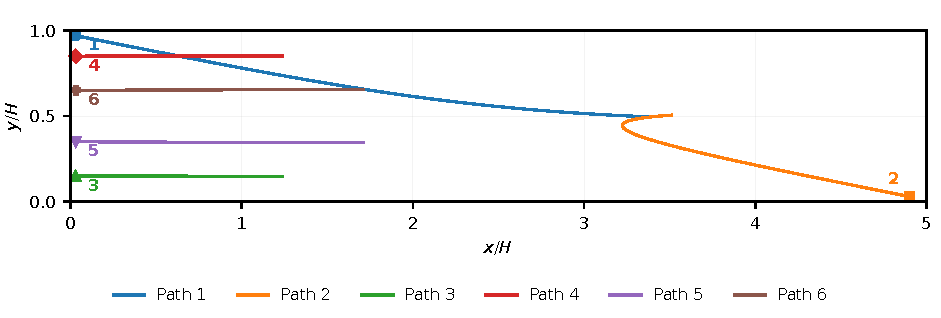
\includegraphics[width=0.92\textwidth]{figs/chapter4/inverse-particle-count-design.pdf}
\caption{ترتیب شش مسیر مرجع در کانال بی‌بعد برای ورودی نه‌نوسانی.}
\label{fig:inverse-count-design}
\end{figure}

مسیرهای مصنوعی از میدان اجزای محدود یا حل تحلیلی پوازوی تولید شدند.
مرجع سهموی از حل تحلیلی به دست آمد.
% REVIEW-AUDIT Y24 | در همهٔ حالت‌ها ثابت ماندند | برازش با تعداد شروع و تکرار محدود انجام شد. | پیشنهاد: بودجهٔ ثابت برازش در مقایسهٔ تعداد ذرات | مرور؛ بودجهٔ محاسباتی محدود | تطبیق با متن گزارش
وزن‌های گام $94000$ و تنظیمات منظم‌سازی \ReviewMark{yellow}{Y24-548-1-1}{در همهٔ حالت‌ها ثابت ماندند}.
پروفایل ورودی با $65$ گره نمایش داده شد.
% REVIEW-AUDIT Y24 | با دو شروع و سقف $200$ تکرار | برازش با تعداد شروع و تکرار محدود انجام شد. | پیشنهاد: بودجهٔ ثابت برازش در مقایسهٔ تعداد ذرات | مرور؛ بودجهٔ محاسباتی محدود | تطبیق با متن گزارش
هر برازش \ReviewMark{yellow}{Y24-550-1-1}{با دو شروع و سقف} \ReviewNumber{yellow}{Y24-550-1-2}{$200$} \ReviewMark{yellow}{Y24-550-1-3}{تکرار} انجام شد.
پاسخ منتخب با کمترین هزینهٔ برازش میان نامزدهای مجاز تعیین شد.
پروفایل حقیقی برای ارزیابی پس از برازش به کار رفت.
معیار شکل~\ref{fig:inverse-count-errors} خطای نسبی پروفایل در مقیاس مشترک $U_{\mathrm{ref}}$ است.
ترتیب پروفایل‌ها برحسب ریشهٔ میانگین مربعات مشتق دوم ورودی است.

\begin{figure}[htbp]
\centering
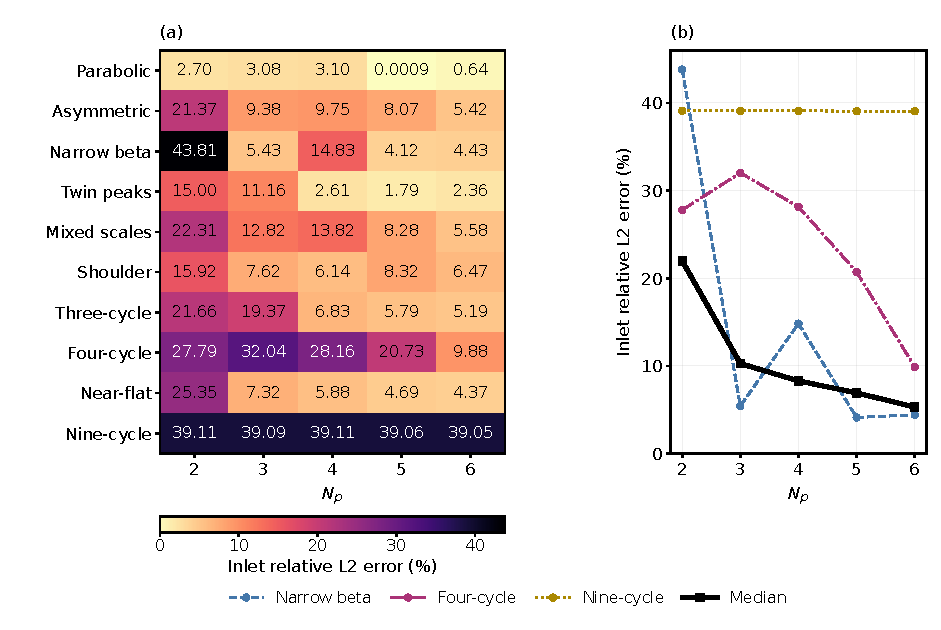
\includegraphics[width=0.98\textwidth]{figs/chapter4/inverse-particle-count-errors.pdf}
% REVIEW-AUDIT Y28 | خطای بازسازی ورودی | نمودار تکرار خطاهای بالا را نشان می‌دهد. | پیشنهاد: خطای بازسازی برحسب ورودی و تعداد ذره | بسیار بالا؛ ضعف کمّی داخل شکل | عنوان در LaTeX علامت خورده است. اعداد داخل تصویر در دارایی اصلی باقی ماندند.
\caption{\ReviewMark{yellow}{Y28-559-1-1}{خطای بازسازی ورودی} برای ده پروفایل و تعدادهای مختلف ذره.}
\label{fig:inverse-count-errors}
\end{figure}

% REVIEW-AUDIT Y25 | میانهٔ خطا از $21.99\%$ برای دو ذره به $5.31\%$ رسید | مقایسه مربوط به میانهٔ خطا در گروه پروفایل‌هاست. | پیشنهاد: میانهٔ خطای پروفایل برحسب تعداد ذرات | بسیار بالا؛ خطای زیاد در دادهٔ کم | تطبیق با متن گزارش
\ReviewMark{yellow}{Y25-563-1-1}{میانهٔ خطا از} \ReviewNumber{yellow}{Y25-563-1-2}{$21.99\%$} \ReviewMark{yellow}{Y25-563-1-3}{برای دو ذره به} \ReviewNumber{yellow}{Y25-563-1-4}{$5.31\%$} \ReviewMark{yellow}{Y25-563-1-5}{رسید}.
خطای شش‌ذره‌ای در هر ده پروفایل از حالت دوذره‌ای کمتر بود.
% REVIEW-AUDIT Y26 | از $40$ افزایش تک‌ذره‌ای، $29$ مورد با کاهش خطا | افزودن یک ذره همیشه خطا را کاهش نداد. | پیشنهاد: بهبود غیر یکنواخت با افزایش تعداد ذرات | بسیار بالا؛ روند غیرتضمینی | تطبیق با متن گزارش
\ReviewMark{yellow}{Y26-565-1-1}{از} \ReviewNumber{yellow}{Y26-565-1-2}{$40$} \ReviewMark{yellow}{Y26-565-1-3}{افزایش تک‌ذره‌ای،} \ReviewNumber{yellow}{Y26-565-1-4}{$29$} \ReviewMark{yellow}{Y26-565-1-5}{مورد با کاهش خطا} همراه بودند.
% REVIEW-AUDIT Y26 | فقط دو پروفایل در همهٔ افزایش‌ها خطای کمتری داشتند | افزودن یک ذره همیشه خطا را کاهش نداد. | پیشنهاد: بهبود غیر یکنواخت با افزایش تعداد ذرات | بسیار بالا؛ روند غیرتضمینی | تطبیق با متن گزارش
\ReviewMark{yellow}{Y26-566-1-1}{فقط دو پروفایل در همهٔ افزایش‌ها خطای کمتری داشتند}.
% REVIEW-AUDIT Y26 | خطا ابتدا کاهش یافت و سپس افزایش یافت | افزودن یک ذره همیشه خطا را کاهش نداد. | پیشنهاد: بهبود غیر یکنواخت با افزایش تعداد ذرات | بسیار بالا؛ روند غیرتضمینی | تطبیق با متن گزارش
در ورودی بتای باریک، \ReviewMark{yellow}{Y26-567-1-1}{خطا ابتدا کاهش یافت و سپس افزایش یافت}.
% REVIEW-AUDIT Y27 | خطای ورودی نه‌نوسانی برای همهٔ تعدادها نزدیک $39\%$ ماند | ورودی نه‌نوسانی در همهٔ تعدادها خطای بالا دارد. | پیشنهاد: پایداری خطای بالای ورودی نه‌نوسانی | بسیار بالا؛ خطای پایدار و زیاد | تطبیق با متن گزارش
\ReviewMark{yellow}{Y27-568-1-1}{خطای ورودی نه‌نوسانی برای همهٔ تعدادها نزدیک} \ReviewNumber{yellow}{Y27-568-1-2}{$39\%$} \ReviewMark{yellow}{Y27-568-1-3}{ماند}.
شکل~\ref{fig:inverse-count-profiles} تغییر شکل پروفایل تخمینی را در چهار نمونه نشان می‌دهد.

\begin{figure}[htbp]
\centering
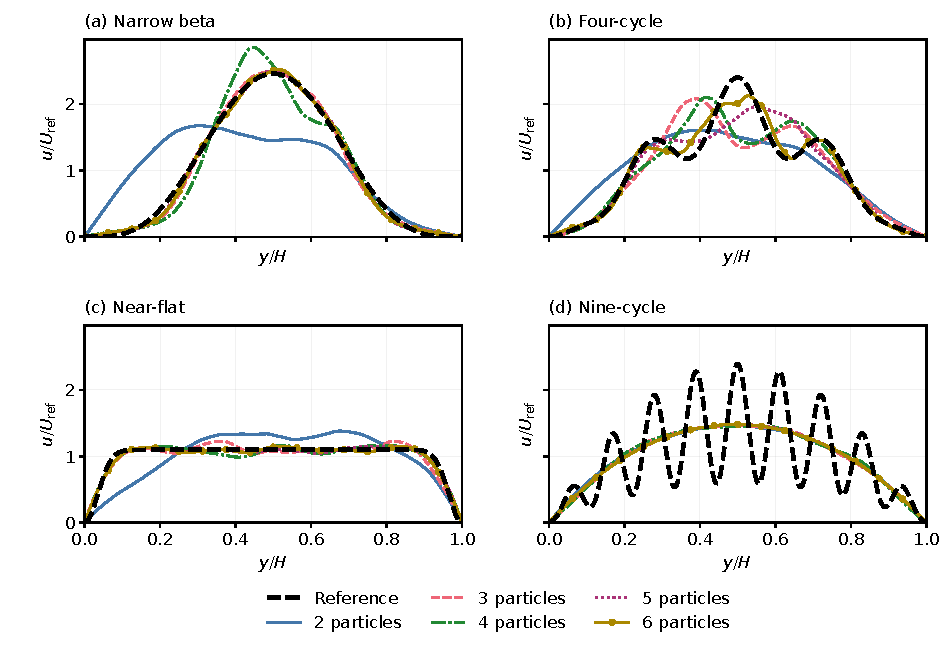
\includegraphics[width=0.95\textwidth]{figs/chapter4/inverse-particle-count-profiles.pdf}
% REVIEW-AUDIT Y28 | پروفایل مرجع و تخمین‌های حاصل | نمودار تکرار خطاهای بالا را نشان می‌دهد. | پیشنهاد: خطای بازسازی برحسب ورودی و تعداد ذره | بسیار بالا؛ ضعف کمّی داخل شکل | عنوان در LaTeX علامت خورده است. اعداد داخل تصویر در دارایی اصلی باقی ماندند.
\caption{\ReviewMark{yellow}{Y28-574-1-1}{پروفایل مرجع و تخمین‌های حاصل} از تعدادهای مختلف ذره.}
\label{fig:inverse-count-profiles}
\end{figure}

% REVIEW-AUDIT Y29 | با شکل پایهٔ مقداردهی اولیه نیز مرتبط است | شکل پایه می‌تواند بر خطای سهموی اثر بگذارد. | پیشنهاد: حساسیت نتیجهٔ سهموی به مقداردهی اولیه | مرور؛ مزیت ناشی از پیش‌دانسته | تطبیق با متن گزارش
خطای بسیار کوچک سهموی \ReviewMark{yellow}{Y29-578-1-1}{با شکل پایهٔ مقداردهی اولیه نیز مرتبط است}.
% REVIEW-AUDIT Y30 | تعداد مشاهدات و پوشش مکانی هم‌زمان تغییر کردند | شمار مشاهده و پوشش مکانی با هم تغییر کردند. | پیشنهاد: اثر مشترک تعداد مشاهده و پوشش مکانی | مرور؛ عامل مخدوش‌کننده و دامنهٔ تعمیم | تطبیق با متن گزارش
در این آزمایش، \ReviewMark{yellow}{Y30-579-1-1}{تعداد مشاهدات و پوشش مکانی هم‌زمان تغییر کردند}.
% REVIEW-AUDIT Y30 | به همین ترتیب رهاسازی و تحقق نویز محدود است | شمار مشاهده و پوشش مکانی با هم تغییر کردند. | پیشنهاد: اثر مشترک تعداد مشاهده و پوشش مکانی | مرور؛ عامل مخدوش‌کننده و دامنهٔ تعمیم | تطبیق با متن گزارش
این مقایسه \ReviewMark{yellow}{Y30-580-1-1}{به همین ترتیب رهاسازی و تحقق نویز محدود است}.
هر $200$ بازپخش به پایان بازهٔ مشاهده رسیدند.
% REVIEW-AUDIT Y31 | همگرایی بهینه‌ساز در هیچ‌یک از $50$ پاسخ منتخب تأیید نشد | گزارش تشخیص همگرایی را برای پاسخ‌های منتخب ثبت نکرد. | پیشنهاد: همگرایی تأییدنشده در بودجهٔ تعیین‌شده | بسیار بالا؛ همگرایی تأییدنشده در کل مجموعه | تطبیق با متن گزارش
\ReviewMark{yellow}{Y31-582-1-1}{همگرایی بهینه‌ساز در هیچ‌یک از} \ReviewNumber{yellow}{Y31-582-1-2}{$50$} \ReviewMark{yellow}{Y31-582-1-3}{پاسخ منتخب تأیید نشد}.
% REVIEW-AUDIT Y31 | با بودجهٔ تعیین‌شده | گزارش تشخیص همگرایی را برای پاسخ‌های منتخب ثبت نکرد. | پیشنهاد: همگرایی تأییدنشده در بودجهٔ تعیین‌شده | بسیار بالا؛ همگرایی تأییدنشده در کل مجموعه | تطبیق با متن گزارش
بنابراین خطاها عملکرد روش را \ReviewMark{yellow}{Y31-583-1-1}{با بودجهٔ تعیین‌شده} نشان می‌دهند.

\clearpage
\زیرقسمت{بازسازی جریان از هندسهٔ مسیرها بدون زمان اندازه‌گیری‌شده}
\label{sec:results-inverse-flow-geometry}

همان سه نمونه با استفاده از منحنی‌های مرتب‌شده بررسی شدند.
نقاط منحنی با فاصلهٔ یکنواخت در طول قوس بازنمونه‌برداری شدند.
% REVIEW-AUDIT Y32 | سرعت اولیهٔ هر ذره همچنان معلوم بود | سرعت اولیه در برازش هندسی معلوم مانده است. | پیشنهاد: برازش هندسی با سرعت اولیهٔ معلوم | مرور؛ اطلاعات جانبی لازم | تطبیق با متن گزارش
\ReviewMark{yellow}{Y32-591-1-1}{سرعت اولیهٔ هر ذره همچنان معلوم بود}.
% REVIEW-AUDIT Y32 | زمان‌های مشاهده و پاسخ زمان‌دار وارد برازش هندسی نشدند | سرعت اولیه در برازش هندسی معلوم مانده است. | پیشنهاد: برازش هندسی با سرعت اولیهٔ معلوم | مرور؛ اطلاعات جانبی لازم | تطبیق با متن گزارش
\ReviewMark{yellow}{Y32-592-1-1}{زمان‌های مشاهده و پاسخ زمان‌دار وارد برازش هندسی نشدند}.
مدت تخمینی، افق بازپخش مستقل هر ذره را تعیین کرد.
هر شش بازپخش در افق تخمینی کامل شدند.

شکل~\ref{fig:results-inverse-geometry} مسیرها و پروفایل‌های تخمینی دو روش را مقایسه می‌کند.
جدول~\ref{tab:results-inverse-geometry} معیارهای مشترک هندسی را برای هر ذره گزارش می‌کند.
تعریف این معیارها در رابطهٔ~\eqref{eq:inverse-flow-geometry-errors} آمده است.
هر دو بازپخش با یک منحنی مشاهده‌شده مقایسه شدند.
% REVIEW-TERM T04 | معیار مرتب | این نام، تعریف ریاضی E_arc را روشن نمی‌کند. رابطهٔ متناظر، خطای نقاط متناظر برحسب طول قوس نرمال‌شده است. | پیشنهاد: خطای تطبیق نقاط برحسب طول قوس نرمال‌شده | اصلاح نام معیار؛ اطمینان بالا | تعریف معیار در متن، تطبیق نقاط روی طول قوس نرمال‌شده است.
در \ReviewMark{blue}{T04-600-1-1}{معیار مرتب}، نقاط متناظر در طول قوس نرمال‌شده مقایسه شدند.

\begin{figure}[htbp]
\centering
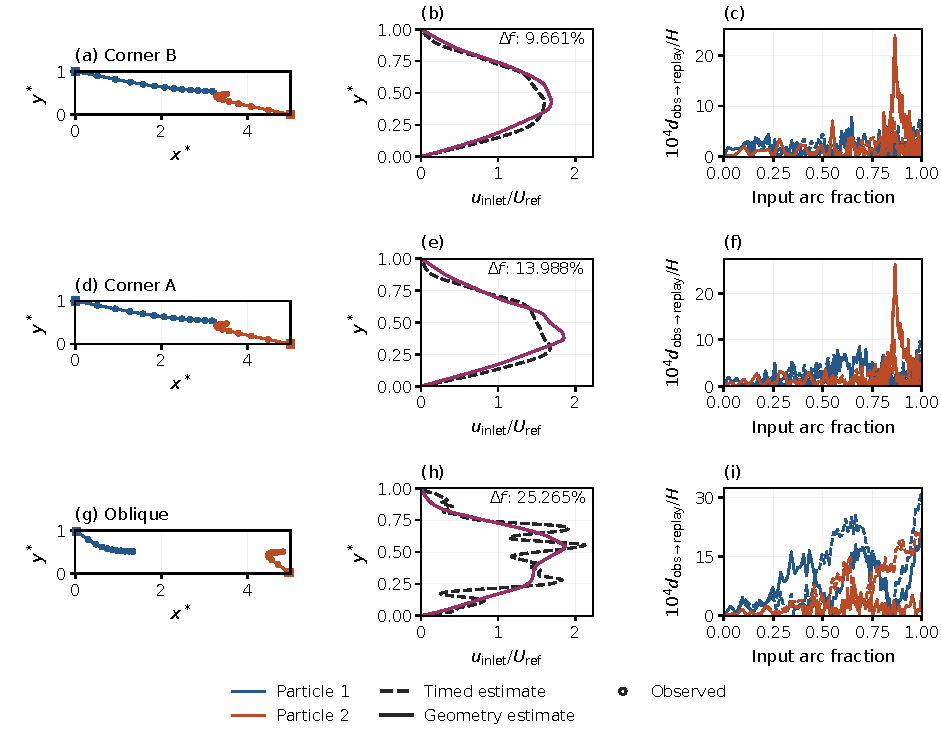
\includegraphics[width=0.97\textwidth,height=0.75\textheight,keepaspectratio]{figs/chapter4/inverse-geometry-comparison.pdf}
% REVIEW-AUDIT Y34 | مقایسهٔ هندسهٔ بازپخش و پروفایل‌های تخمینی | اختلاف نسبی نسبت به تخمین زمان‌دار محاسبه شده است. | پیشنهاد: اختلاف دو تخمین با مبنای روش زمان‌دار | مرور؛ ناپایداری تخمین و تفاوت روش‌ها | تطبیق با متن گزارش
\caption{\ReviewMark{yellow}{Y34-605-1-1}{مقایسهٔ هندسهٔ بازپخش و پروفایل‌های تخمینی} در دو روش.}
\label{fig:results-inverse-geometry}
\end{figure}

\begin{table}[htbp]
\centering
\small
\setlength{\tabcolsep}{5pt}
% REVIEW-AUDIT Y33 | خطاهای هندسی بی‌بعد دو بازپخش | دو معیار ذرهٔ دوم در هر دو سناریو بدتر شدند. | پیشنهاد: افزایش خطای هندسی ذرهٔ دوم | مرور؛ افت عملکرد بعضی مسیرها | تطبیق با متن گزارش
\caption{\ReviewMark{yellow}{Y33-613-1-1}{خطاهای هندسی بی‌بعد دو بازپخش} با مقیاس مشترک.}
\label{tab:results-inverse-geometry}
\begin{tabular}{@{}lccccc@{}}
\hline
 & & \multicolumn{2}{c}{$10^4 E_{\mathrm{sym}}^*$}
     & \multicolumn{2}{c}{$10^4 E_{\mathrm{arc}}^*$} \\
نمونه & ذره & زمان‌دار & بدون زمان & زمان‌دار & بدون زمان \\
\hline
% REVIEW-TERM T19 | گوشه‌ای ب | در متن، تعریف کافی برای گوشه‌ای دیده نمی‌شود. corner case الزاماً به ذرات نزدیک گوشهٔ کانال اشاره ندارد. نام اصلی و تنظیمات نمونه باید بررسی شوند. | پیشنهاد: سناریوی رهاسازی از دو گوشهٔ مقابل، با شناسهٔ الف یا ب | شناسهٔ نامفهوم؛ نیازمند بررسی منبع | الف corners_beta5 و ب corners_beta4 است. هر دو از گوشه‌های بالاچپ و پایین‌راست شروع می‌کنند.
\ReviewMark{blue}{T19-621-1-1}{گوشه‌ای ب} & $1$ & $2.713$ & $2.130$ & $6.467$ & $2.134$ \\
% REVIEW-TERM T19 | گوشه‌ای ب | در متن، تعریف کافی برای گوشه‌ای دیده نمی‌شود. corner case الزاماً به ذرات نزدیک گوشهٔ کانال اشاره ندارد. نام اصلی و تنظیمات نمونه باید بررسی شوند. | پیشنهاد: سناریوی رهاسازی از دو گوشهٔ مقابل، با شناسهٔ الف یا ب | شناسهٔ نامفهوم؛ نیازمند بررسی منبع | الف corners_beta5 و ب corners_beta4 است. هر دو از گوشه‌های بالاچپ و پایین‌راست شروع می‌کنند.؛ مرتبط Y33
% REVIEW-AUDIT Y33 | $2.059$ | دو معیار ذرهٔ دوم در هر دو سناریو بدتر شدند. | پیشنهاد: افزایش خطای هندسی ذرهٔ دوم | مرور؛ افت عملکرد بعضی مسیرها | تطبیق با متن گزارش؛ مرتبط T19
% REVIEW-AUDIT Y33 | $4.030$ | دو معیار ذرهٔ دوم در هر دو سناریو بدتر شدند. | پیشنهاد: افزایش خطای هندسی ذرهٔ دوم | مرور؛ افت عملکرد بعضی مسیرها | تطبیق با متن گزارش؛ مرتبط T19
% REVIEW-AUDIT Y33 | $8.432$ | دو معیار ذرهٔ دوم در هر دو سناریو بدتر شدند. | پیشنهاد: افزایش خطای هندسی ذرهٔ دوم | مرور؛ افت عملکرد بعضی مسیرها | تطبیق با متن گزارش؛ مرتبط T19
% REVIEW-AUDIT Y33 | $19.779$ | دو معیار ذرهٔ دوم در هر دو سناریو بدتر شدند. | پیشنهاد: افزایش خطای هندسی ذرهٔ دوم | مرور؛ افت عملکرد بعضی مسیرها | تطبیق با متن گزارش؛ مرتبط T19
\ReviewMark{blue}{T19-622-1-1}{گوشه‌ای ب} & $2$ & \ReviewNumber{yellow}{Y33-622-2-1}{$2.059$} & \ReviewNumber{yellow}{Y33-622-3-1}{$4.030$} & \ReviewNumber{yellow}{Y33-622-4-1}{$8.432$} & \ReviewNumber{yellow}{Y33-622-5-1}{$19.779$} \\
% REVIEW-TERM T19 | گوشه‌ای الف | در متن، تعریف کافی برای گوشه‌ای دیده نمی‌شود. corner case الزاماً به ذرات نزدیک گوشهٔ کانال اشاره ندارد. نام اصلی و تنظیمات نمونه باید بررسی شوند. | پیشنهاد: سناریوی رهاسازی از دو گوشهٔ مقابل، با شناسهٔ الف یا ب | شناسهٔ نامفهوم؛ نیازمند بررسی منبع | الف corners_beta5 و ب corners_beta4 است. هر دو از گوشه‌های بالاچپ و پایین‌راست شروع می‌کنند.
\ReviewMark{blue}{T19-623-1-1}{گوشه‌ای الف} & $1$ & $3.388$ & $3.149$ & $7.773$ & $3.152$ \\
% REVIEW-TERM T19 | گوشه‌ای الف | در متن، تعریف کافی برای گوشه‌ای دیده نمی‌شود. corner case الزاماً به ذرات نزدیک گوشهٔ کانال اشاره ندارد. نام اصلی و تنظیمات نمونه باید بررسی شوند. | پیشنهاد: سناریوی رهاسازی از دو گوشهٔ مقابل، با شناسهٔ الف یا ب | شناسهٔ نامفهوم؛ نیازمند بررسی منبع | الف corners_beta5 و ب corners_beta4 است. هر دو از گوشه‌های بالاچپ و پایین‌راست شروع می‌کنند.؛ مرتبط Y33
% REVIEW-AUDIT Y33 | $2.219$ | دو معیار ذرهٔ دوم در هر دو سناریو بدتر شدند. | پیشنهاد: افزایش خطای هندسی ذرهٔ دوم | مرور؛ افت عملکرد بعضی مسیرها | تطبیق با متن گزارش؛ مرتبط T19
% REVIEW-AUDIT Y33 | $4.238$ | دو معیار ذرهٔ دوم در هر دو سناریو بدتر شدند. | پیشنهاد: افزایش خطای هندسی ذرهٔ دوم | مرور؛ افت عملکرد بعضی مسیرها | تطبیق با متن گزارش؛ مرتبط T19
% REVIEW-AUDIT Y33 | $10.850$ | دو معیار ذرهٔ دوم در هر دو سناریو بدتر شدند. | پیشنهاد: افزایش خطای هندسی ذرهٔ دوم | مرور؛ افت عملکرد بعضی مسیرها | تطبیق با متن گزارش؛ مرتبط T19
% REVIEW-AUDIT Y33 | $21.478$ | دو معیار ذرهٔ دوم در هر دو سناریو بدتر شدند. | پیشنهاد: افزایش خطای هندسی ذرهٔ دوم | مرور؛ افت عملکرد بعضی مسیرها | تطبیق با متن گزارش؛ مرتبط T19
\ReviewMark{blue}{T19-624-1-1}{گوشه‌ای الف} & $2$ & \ReviewNumber{yellow}{Y33-624-2-1}{$2.219$} & \ReviewNumber{yellow}{Y33-624-3-1}{$4.238$} & \ReviewNumber{yellow}{Y33-624-4-1}{$10.850$} & \ReviewNumber{yellow}{Y33-624-5-1}{$21.478$} \\
مایل & $1$ & $13.067$ & $9.523$ & $14.242$ & $10.932$ \\
مایل & $2$ & $8.795$ & $2.264$ & $15.992$ & $4.228$ \\
\hline
\end{tabular}
\end{table}

در چهار مسیر، هر دو خطای هندسی با روش بدون زمان کاهش یافتند.
% REVIEW-TERM T19 | دو نمونهٔ گوشه‌ای | در متن، تعریف کافی برای گوشه‌ای دیده نمی‌شود. corner case الزاماً به ذرات نزدیک گوشهٔ کانال اشاره ندارد. نام اصلی و تنظیمات نمونه باید بررسی شوند. | پیشنهاد: سناریوی رهاسازی از دو گوشهٔ مقابل، با شناسهٔ الف یا ب | شناسهٔ نامفهوم؛ نیازمند بررسی منبع | الف corners_beta5 و ب corners_beta4 است. هر دو از گوشه‌های بالاچپ و پایین‌راست شروع می‌کنند.؛ مرتبط Y34
% REVIEW-AUDIT Y34 | در هر دو نمونهٔ گوشه‌ای، خطاهای ذرهٔ دوم افزایش یافتند | اختلاف نسبی نسبت به تخمین زمان‌دار محاسبه شده است. | پیشنهاد: اختلاف دو تخمین با مبنای روش زمان‌دار | مرور؛ ناپایداری تخمین و تفاوت روش‌ها | تطبیق با متن گزارش؛ مرتبط T19
\ReviewMark{yellow}{Y34-632-2-1}{در هر} \ReviewMark{blue}{T19-632-1-1}{دو نمونهٔ گوشه‌ای}\ReviewMark{yellow}{Y34-632-2-3}{، خطاهای ذرهٔ دوم افزایش یافتند}.
% REVIEW-AUDIT Y34 | $2.62\times10^{-3}$ | اختلاف نسبی نسبت به تخمین زمان‌دار محاسبه شده است. | پیشنهاد: اختلاف دو تخمین با مبنای روش زمان‌دار | مرور؛ ناپایداری تخمین و تفاوت روش‌ها | تطبیق با متن گزارش
بیشینهٔ فاصلهٔ هاوسدورف در روش بدون زمان حدود \ReviewNumber{yellow}{Y34-633-1-1}{$2.62\times10^{-3}$} بود.
% REVIEW-AUDIT Y34 | از $9.661\%$ تا $25.265\%$ | اختلاف نسبی نسبت به تخمین زمان‌دار محاسبه شده است. | پیشنهاد: اختلاف دو تخمین با مبنای روش زمان‌دار | مرور؛ ناپایداری تخمین و تفاوت روش‌ها | تطبیق با متن گزارش
اختلاف نسبی پروفایل‌ها در سه نمونه \ReviewMark{yellow}{Y34-634-1-1}{از} \ReviewNumber{yellow}{Y34-634-1-2}{$9.661\%$} \ReviewMark{yellow}{Y34-634-1-3}{تا} \ReviewNumber{yellow}{Y34-634-1-4}{$25.265\%$} بود.
% REVIEW-AUDIT Y34 | مبنای این اختلاف، پروفایل تخمینی روش زمان‌دار است | اختلاف نسبی نسبت به تخمین زمان‌دار محاسبه شده است. | پیشنهاد: اختلاف دو تخمین با مبنای روش زمان‌دار | مرور؛ ناپایداری تخمین و تفاوت روش‌ها | تطبیق با متن گزارش
\ReviewMark{yellow}{Y34-635-1-1}{مبنای این اختلاف، پروفایل تخمینی روش زمان‌دار است}.
% REVIEW-AUDIT Y34 | اختلاف شکل همچنان دیده شد | اختلاف نسبی نسبت به تخمین زمان‌دار محاسبه شده است. | پیشنهاد: اختلاف دو تخمین با مبنای روش زمان‌دار | مرور؛ ناپایداری تخمین و تفاوت روش‌ها | تطبیق با متن گزارش
با نرمال‌سازی هر پروفایل بر میانگین خودش، \ReviewMark{yellow}{Y34-636-1-1}{اختلاف شکل همچنان دیده شد}.
% REVIEW-AUDIT Y34 | $25.258\%$ | اختلاف نسبی نسبت به تخمین زمان‌دار محاسبه شده است. | پیشنهاد: اختلاف دو تخمین با مبنای روش زمان‌دار | مرور؛ ناپایداری تخمین و تفاوت روش‌ها | تطبیق با متن گزارش
بزرگ‌ترین اختلاف شکل در نمونهٔ مایل، برابر \ReviewNumber{yellow}{Y34-637-1-1}{$25.258\%$} بود.

شکل~\ref{fig:results-inverse-duration} مدت تخمینی را با مدت مشاهده مقایسه می‌کند.
در روش زمان‌دار، مدت حرکت از داده معلوم بود.
در روش بدون زمان، این مدت از زمان‌بندی تخمینی به دست آمد.
مدت مشاهده فقط در ارزیابی پس از برازش استفاده شد.
% REVIEW-AUDIT Y35 | بزرگ‌ترین اختلاف نسبی مدت، $4.393\%$ | اختلاف مدت نسبت به مشاهده سنجیده شد. | پیشنهاد: اختلاف مدت تخمینی با مدت مشاهده | مرور؛ اختلاف زمانی محدود | تطبیق با متن گزارش
\ReviewMark{yellow}{Y35-643-1-1}{بزرگ‌ترین اختلاف نسبی مدت،} \ReviewNumber{yellow}{Y35-643-1-2}{$4.393\%$}، برای ذرهٔ اول نمونهٔ مایل بود.
% REVIEW-AUDIT Y35 | $0.55$ | اختلاف مدت نسبت به مشاهده سنجیده شد. | پیشنهاد: اختلاف مدت تخمینی با مدت مشاهده | مرور؛ اختلاف زمانی محدود | تطبیق با متن گزارش
% REVIEW-AUDIT Y35 | $0.574160$ | اختلاف مدت نسبت به مشاهده سنجیده شد. | پیشنهاد: اختلاف مدت تخمینی با مدت مشاهده | مرور؛ اختلاف زمانی محدود | تطبیق با متن گزارش
در آن مسیر، مدت مشاهده \ReviewNumber{yellow}{Y35-644-1-1}{$0.55$} و مدت تخمینی \ReviewNumber{yellow}{Y35-644-2-1}{$0.574160$} بود.
این مدت به انتهای منحنی برازش‌شده مربوط است.

\begin{figure}[htbp]
\centering
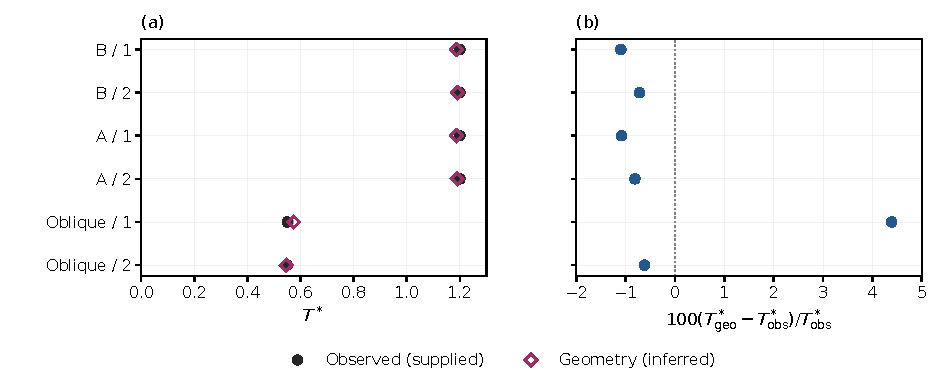
\includegraphics[width=0.95\textwidth]{figs/chapter4/inverse-geometry-duration.pdf}
% REVIEW-AUDIT Y35 | مقایسهٔ مدت بی‌بعد مشاهده و مدت تخمینی | اختلاف مدت نسبت به مشاهده سنجیده شد. | پیشنهاد: اختلاف مدت تخمینی با مدت مشاهده | مرور؛ اختلاف زمانی محدود | تطبیق با متن گزارش
\caption{\ReviewMark{yellow}{Y35-650-1-1}{مقایسهٔ مدت بی‌بعد مشاهده و مدت تخمینی} هر مسیر.}
\label{fig:results-inverse-duration}
\end{figure}

% REVIEW-AUDIT Y36 | هر دو شروع به سقف $700$ تکرار رسیدند | بودجه و تنظیمات روش‌ها یکسان نبودند. | پیشنهاد: مقایسهٔ روش‌ها با بودجه‌های متفاوت | مرور؛ همگرایی و محدودیت مقایسهٔ علّی | تطبیق با متن گزارش
در روش بدون زمان، \ReviewMark{yellow}{Y36-654-1-1}{هر دو شروع به سقف} \ReviewNumber{yellow}{Y36-654-1-2}{$700$} \ReviewMark{yellow}{Y36-654-1-3}{تکرار رسیدند}.
% REVIEW-AUDIT Y36 | تنظیمات و بودجهٔ بهینه‌سازی دو روش متفاوت بودند | بودجه و تنظیمات روش‌ها یکسان نبودند. | پیشنهاد: مقایسهٔ روش‌ها با بودجه‌های متفاوت | مرور؛ همگرایی و محدودیت مقایسهٔ علّی | تطبیق با متن گزارش
\ReviewMark{yellow}{Y36-655-1-1}{تنظیمات و بودجهٔ بهینه‌سازی دو روش متفاوت بودند}.
% REVIEW-AUDIT Y36 | نمی‌توان فقط به حذف زمان نسبت داد | بودجه و تنظیمات روش‌ها یکسان نبودند. | پیشنهاد: مقایسهٔ روش‌ها با بودجه‌های متفاوت | مرور؛ همگرایی و محدودیت مقایسهٔ علّی | تطبیق با متن گزارش
بنابراین اختلاف نتایج را \ReviewMark{yellow}{Y36-656-1-1}{نمی‌توان فقط به حذف زمان نسبت داد}.

\زیرقسمت{رهگیری مسیر هدف با تحریک مغناطیسی در مدل نهم}
\label{sec:results-master9-tracking}

چهار سناریوی رهگیری در جریان پوازوی لولهٔ مستقیم بررسی شدند.
نمای طولی لوله به‌شکل یک ناحیهٔ مستطیلی نمایش داده می‌شود.
مقیاس‌های $X$، $Z$ و $\tau$ مطابق رابطهٔ~\eqref{eq:forward-mag-scales} هستند.
مسیر هدف با مختصات محوری $Z$ تعریف شد.
گام بی‌بعد انتخاب تحریک برابر $0.025$ بود.
تحریک مؤثر هر گام طبق رابطهٔ~\eqref{eq:inverse-master9-tracking} انتخاب شد.
همان دنبالهٔ تحریک با حل‌گر اینرسی‌دار \lr{Radau} بازپخش شد.

مقیاس طولی و عرضی بر طول‌های مرجع متفاوت استوارند.
بازهٔ نمایش مسیر با دامنهٔ حرکت هر سناریو تنظیم شده است.
فرمان مثبت منبع راست و فرمان منفی منبع چپ را فعال می‌کند.
در فرمان صفر، میدان مغناطیسی خاموش است.
% REVIEW-AUDIT Y37 | جریان اندازه‌گیری‌شدهٔ سیم‌پیچ نیست | فرمان مؤثر با جریان اندازه‌گیری‌شدهٔ سیم‌پیچ فرق دارد. | پیشنهاد: فرمان مؤثر مدل با تفسیر مشخص | مرور؛ دامنهٔ تفسیر فرمان | تطبیق با متن گزارش
این فرمان، \ReviewMark{yellow}{Y37-673-1-1}{جریان اندازه‌گیری‌شدهٔ سیم‌پیچ نیست}.

شکل~\ref{fig:results-master9-tracking} مسیر هدف و بازپخش دو سناریو را نشان می‌دهد.
پنل‌ها تحریک پله‌ای و خطای عرضی رهگیری را نیز نشان می‌دهند.
برای سنجش خطا، هدف در مکان محوری بازپخش ارزیابی شد.
اختلاف دو حل در زمان‌های یکسان محاسبه شد.

\begin{figure}[htbp]
\centering
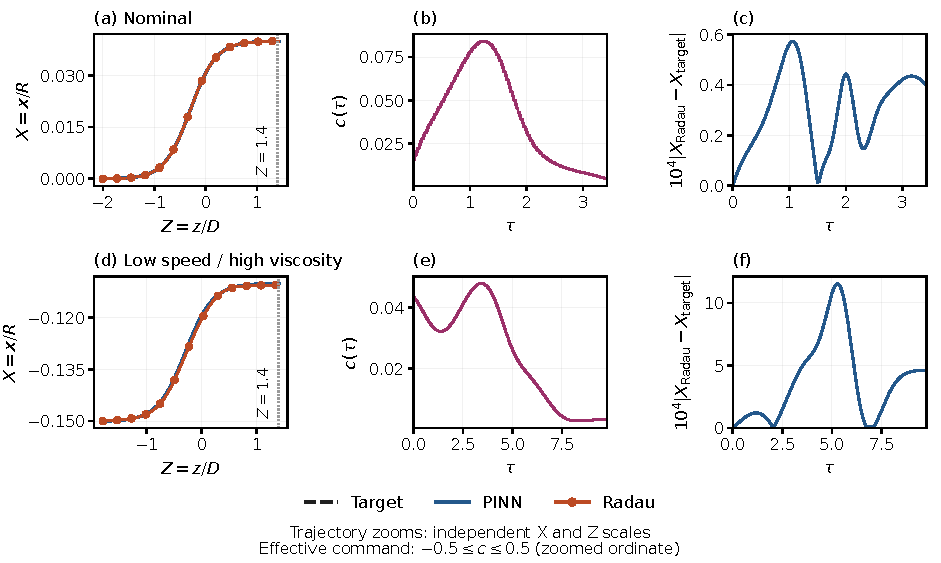
\includegraphics[width=0.98\textwidth,height=0.72\textheight,keepaspectratio]{figs/chapter4/inverse-master9-tracking.pdf}
% REVIEW-AUDIT Y38 | حالت اسمی و حالت کم‌سرعت | اعتبار این مقایسه به خانوادهٔ مسیرهای آزموده‌شده محدود است. | پیشنهاد: رهگیری در خانوادهٔ مسیرهای هدف هموار | مرور؛ ضعف نسبی و دامنهٔ آزمون | هر چهار سناریوی رهگیری از معیارهای گزارش‌شده عبور کردند.
\caption{مسیر، تحریک و خطای رهگیری در \ReviewMark{yellow}{Y38-683-1-1}{حالت اسمی و حالت کم‌سرعت}.}
\label{fig:results-master9-tracking}
\end{figure}

جدول~\ref{tab:results-master9-tracking} خطا و موقعیت محوری نهایی را گزارش می‌کند.
خطای رهگیری مطابق رابطهٔ~\eqref{eq:validation-master9-tracking} تعریف شد.
آستانهٔ پایان برای مسیر شبکه $Z=1.4$ بود.
شرط تکمیل برای بازپخش، رسیدن به دست‌کم $Z=1.3$ بود.
بازپخش هر چهار سناریو از $Z=1.4$ نیز عبور کرد.

\begin{table}[htbp]
\centering
\small
\setlength{\tabcolsep}{4pt}
\renewcommand{\arraystretch}{0.85}
\caption{خطاهای بی‌بعد و وضعیت تکمیل رهگیری در چهار سناریو.}
\label{tab:results-master9-tracking}
\begin{tabular}{@{}lcccccc@{}}
\hline
سناریو & $\mathrm{Re}$ & $10^4 E_{\mathrm{track},\infty}$ &
$10^4\Delta X_{\max}$ & $10^4\Delta Z_{\max}$ &
$Z_{\mathrm{Radau},f}$ & تکمیل \\
\hline
اسمی & $0.687$ & $0.572$ & $0.595$ & $8.052$ & $1.42266$ & بله \\
سرعت کم و گرانروی زیاد & $0.125$ & $11.529$ & $11.506$ & $2.592$ & $1.40304$ & بله \\
رینولدز زیاد و رهاسازی سریع & $4.950$ & $1.123$ & $1.122$ & $3.009$ & $1.40466$ & بله \\
رهاسازی جابه‌جاشده & $0.7125$ & $0.413$ & $0.451$ & $2.502$ & $1.40170$ & بله \\
\hline
\end{tabular}
\end{table}

$\Delta X_{\max}$ و $\Delta Z_{\max}$ بیشینهٔ اختلاف مکانی دو حل هستند.
% REVIEW-AUDIT Y38 | بیشترین خطای عرضی رهگیری | اعتبار این مقایسه به خانوادهٔ مسیرهای آزموده‌شده محدود است. | پیشنهاد: رهگیری در خانوادهٔ مسیرهای هدف هموار | مرور؛ ضعف نسبی و دامنهٔ آزمون | هر چهار سناریوی رهگیری از معیارهای گزارش‌شده عبور کردند.
حالت کم‌سرعت \ReviewMark{yellow}{Y38-715-1-1}{بیشترین خطای عرضی رهگیری} را داشت.
% REVIEW-AUDIT Y38 | بیشترین اختلاف محوری دو حل | اعتبار این مقایسه به خانوادهٔ مسیرهای آزموده‌شده محدود است. | پیشنهاد: رهگیری در خانوادهٔ مسیرهای هدف هموار | مرور؛ ضعف نسبی و دامنهٔ آزمون | هر چهار سناریوی رهگیری از معیارهای گزارش‌شده عبور کردند.
\ReviewMark{yellow}{Y38-716-1-1}{بیشترین اختلاف محوری دو حل} در حالت اسمی ثبت شد.
هر چهار سناریو معیارهای عددی رهگیری را برآورده کردند.
% REVIEW-TERM T05 | مسیرهای هدف نرم | در این بافت، smooth به همواری مسیر اشاره دارد. نرم ممکن است ویژگی مکانیکی یا قید نرم را القا کند. | پیشنهاد: مسیرهای هدف هموار | اصلاح ترجمه؛ اطمینان بالا | صفت به خانوادهٔ مسیرهای هدف مربوط است. این پیشنهاد نگارشی است.؛ مرتبط Y38
% REVIEW-AUDIT Y38 | خانوادهٔ مسیرهای هدف نرم | اعتبار این مقایسه به خانوادهٔ مسیرهای آزموده‌شده محدود است. | پیشنهاد: رهگیری در خانوادهٔ مسیرهای هدف هموار | مرور؛ ضعف نسبی و دامنهٔ آزمون | هر چهار سناریوی رهگیری از معیارهای گزارش‌شده عبور کردند.؛ مرتبط T05
این مقایسه برای \ReviewMark{yellow}{Y38-718-2-1}{خانوادهٔ} \ReviewMark{blue}{T05-718-1-1}{مسیرهای هدف نرم} انجام شد.

\clearpage
\زیرقسمت{بازیابی تحریک مغناطیسی از مسیر زمان‌دار ذره}
\label{sec:results-master10-inverse-pending}

% REVIEW-AUDIT Y39 | موقعیت‌های زمان‌دار مصنوعی | بازسازی با هندسه، جریان و شرط اولیهٔ معلوم انجام شد. | پیشنهاد: آزمون مصنوعی با پارامترهای معلوم و ثابت | مرور؛ دامنهٔ اطلاعات و آزمایش | تطبیق با متن گزارش
\ReviewMark{yellow}{Y39-724-1-1}{موقعیت‌های زمان‌دار مصنوعی} برای بازیابی دو دامنهٔ منبع استفاده شدند.
% REVIEW-AUDIT Y39 | جریان حامل، هندسه و پارامترهای سیال معلوم و ثابت بودند | بازسازی با هندسه، جریان و شرط اولیهٔ معلوم انجام شد. | پیشنهاد: آزمون مصنوعی با پارامترهای معلوم و ثابت | مرور؛ دامنهٔ اطلاعات و آزمایش | تطبیق با متن گزارش
\ReviewMark{yellow}{Y39-725-1-1}{جریان حامل، هندسه و پارامترهای سیال معلوم و ثابت بودند}.
% REVIEW-AUDIT Y39 | به سرعت اولیهٔ مستقل نیاز ندارد | بازسازی با هندسه، جریان و شرط اولیهٔ معلوم انجام شد. | پیشنهاد: آزمون مصنوعی با پارامترهای معلوم و ثابت | مرور؛ دامنهٔ اطلاعات و آزمایش | تطبیق با متن گزارش
مدل بیش‌میرا \ReviewMark{yellow}{Y39-726-1-1}{به سرعت اولیهٔ مستقل نیاز ندارد}.
% REVIEW-AUDIT Y39 | از اولین موقعیت دقیق | بازسازی با هندسه، جریان و شرط اولیهٔ معلوم انجام شد. | پیشنهاد: آزمون مصنوعی با پارامترهای معلوم و ثابت | مرور؛ دامنهٔ اطلاعات و آزمایش | تطبیق با متن گزارش
شرط اولیه \ReviewMark{yellow}{Y39-727-1-1}{از اولین موقعیت دقیق} گرفته شد.
% REVIEW-AUDIT Y39 | در تمام برازش‌ها ثابت ماندند | بازسازی با هندسه، جریان و شرط اولیهٔ معلوم انجام شد. | پیشنهاد: آزمون مصنوعی با پارامترهای معلوم و ثابت | مرور؛ دامنهٔ اطلاعات و آزمایش | تطبیق با متن گزارش
وزن‌های آموزش‌دیدهٔ مدل دهم \ReviewMark{yellow}{Y39-728-1-1}{در تمام برازش‌ها ثابت ماندند}.
روش از هدف رابطهٔ~\eqref{eq:inverse-master10-proposed-objective} استفاده می‌کند.

در آزمون پایه، هفت گره روی بازهٔ $[0,1.5]$ قرار داشتند.
بین گره‌ها از درون‌یابی خطی استفاده شد.
پنجرهٔ پایه برابر $0.0125$ و محاسبات از نوع \lr{float64} بود.
معیار انتخاب شروع، مجموع هزینهٔ داده و جریمه‌های اعلام‌شده بود.
شروع‌ها غیرصفر و مستقل از تحریک حقیقی انتخاب شدند.
تحریک مرجع فقط در تولید مشاهده و ارزیابی استفاده شد.
بازپخش مستقل، ضرایب خام تخمینی را دریافت کرد.

در آزمون $A$، فقط منبع چپِ مثبت مجهول بود.
در آزمون $B$، هر دو منبع بدون پیشین علامت تخمین زده شدند.
هر دو آزمون از موقعیت اولیهٔ $(X_0,Z_0)=(0.12,-1)$ آغاز شدند.
هر مسیر پایه $121$ مشاهده داشت.
ارزیابی مستقل روی $601$ زمان مشترک انجام شد.
% REVIEW-TERM T06 | تحریک نرم تغییر منبع | منظور، تحریک با تغییرات زمانی هموار است. بایگانی‌شده الزاماً غلط نیست، اما شناسهٔ اجرای مرجع باید مشخص باشد. | پیشنهاد: تحریک هموار با تغییر منبع / تحریک هموارِ ذخیره‌شده | اصلاح ترجمه؛ اطمینان بالا | اجرای C_switch تحریک هموار با تانژانت هذلولوی دارد. مسیر مرجع از آرشیو 05_source_switch.csv خوانده می‌شود.
آزمون $C$ از حل عددیِ \ReviewMark{blue}{T06-744-1-1}{تحریک نرم تغییر منبع} استفاده کرد.
افق زمانی این آزمون $2.25$ بود.

شکل~\ref{fig:results-master10-controls} تحریک حقیقی و تخمینی دو آزمون را نشان می‌دهد.
برای مقایسه، یک علامت مشترک برای هر دو منبع انتخاب شد.
این علامت در همهٔ زمان‌ها ثابت ماند.
معیار مقایسه مطابق رابطهٔ~\eqref{eq:validation-master10-proposed-recovery} است.

\begin{figure}[htbp]
\centering
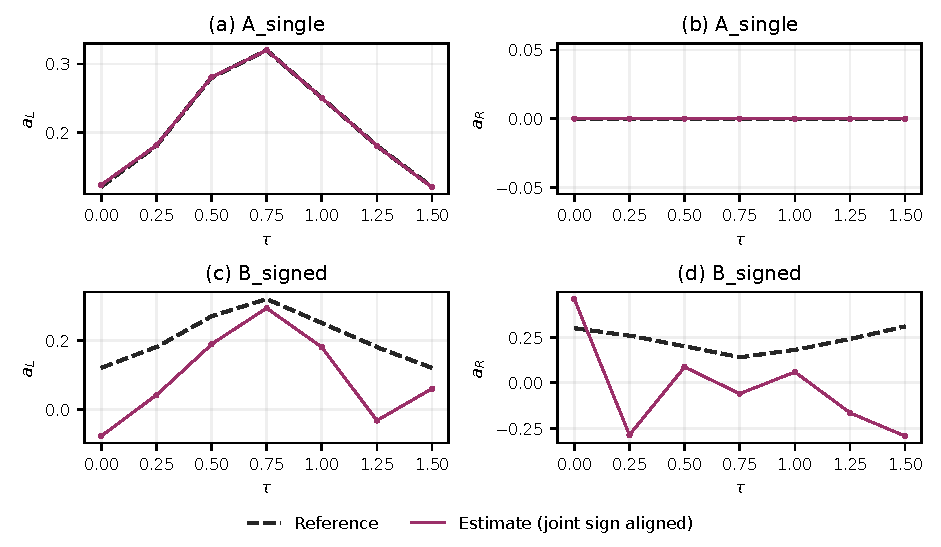
\includegraphics[width=0.98\textwidth]{figs/chapter4/inverse-master10-controls.pdf}
% REVIEW-TERM T10 | تخمین هم‌تراز | طبق معیار E_a، تنها یک علامت سراسری مشترک برای دو منبع انتخاب می‌شود. منظور جابه‌جایی زمانی یا تطبیق دامنه نیست. | پیشنهاد: تخمین با علامت تطبیق‌یافته / پس از تطبیق علامت سراسری دو منبع | رفع ابهام؛ اطمینان بالا | یک علامت ثابت بر کل آرایهٔ دومنبعی اعمال می‌شود. نمونهٔ تک‌منبع مثبت علامت معلوم دارد.؛ مرتبط Y41
% REVIEW-AUDIT Y41 | آزمون‌های تک‌منبعی و دومنبعی | خطای تحریک از خطای مسیر جداست. | پیشنهاد: خطای بازیابی تحریک و وضعیت توقف به تفکیک | بسیار بالا؛ بازیابی ناموفق یا کم‌دقت تحریک | شروع منتخب A_single شاخص 1 دارد. پیام ثبت‌شده «ABNORMAL: » و همگرایی false است. جزئیات بیشترِ توقف در پیام نیامده است.؛ مرتبط T10
\caption{تحریک مرجع و \ReviewMark{blue}{T10-755-1-1}{تخمین هم‌تراز} در \ReviewMark{yellow}{Y41-755-2-1}{آزمون‌های تک‌منبعی و دومنبعی}.}
\label{fig:results-master10-controls}
\end{figure}

شکل~\ref{fig:results-master10-replay} پیش‌بینی شبکه و بازپخش مستقل را مقایسه می‌کند.
بازپخش با حل‌گر \lr{DOP853} و معادلهٔ اصلی انجام شد.
مقیاس‌های عرضی و محوری، طول‌های مرجع متفاوت دارند.
قاب مسیر بزرگ‌نمایی شده و مرز آن دیوارهٔ لوله نیست.
خطای هر مؤلفه جداگانه و با مقیاس ثابت گزارش می‌شود.

\begin{figure}[htbp]
\centering
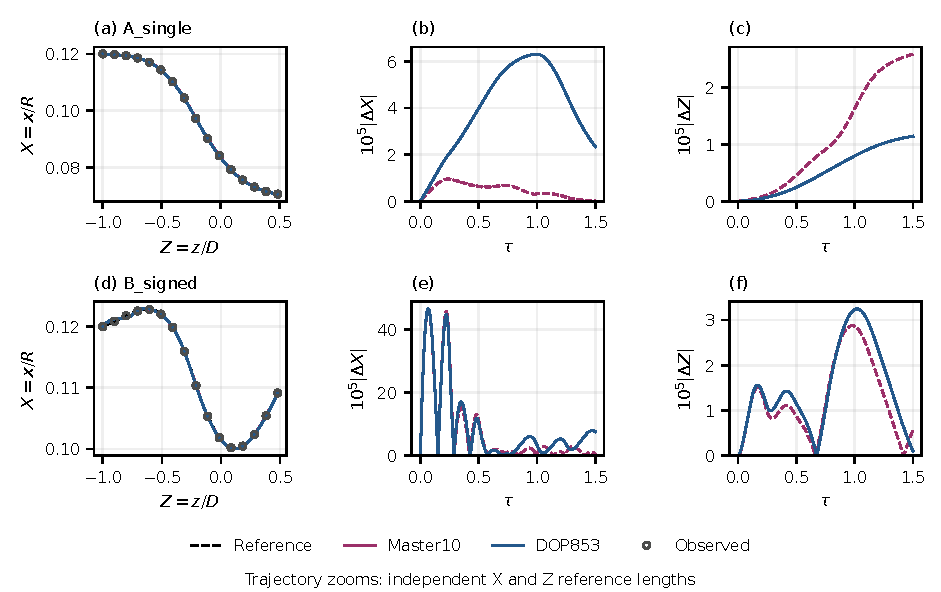
\includegraphics[width=0.98\textwidth]{figs/chapter4/inverse-master10-replay.pdf}
\caption{مسیر تخمینی و بازپخش مستقل همراه خطاهای بی‌بعد دو مؤلفه.}
\label{fig:results-master10-replay}
\end{figure}

% REVIEW-TERM T29 | مرجع پاک | منظور مسیر مرجع پیش از افزودن نویز است. پاک ترجمه‌ای تحت‌اللفظی است و الزاماً خطای علمی ندارد. | پیشنهاد: مرجع بدون نویز | پیشنهاد اختیاری؛ پیشنهاد نگارشی؛ اطمینان متوسط | clean پیش از افزودن نویز ساخته می‌شود. مشاهدهٔ اول دقیق نگه داشته می‌شود.؛ مرتبط Y40
% REVIEW-AUDIT Y40 | نسبت به مرجع پاک | وضعیت توقف به شروع منتخب و بودجهٔ محدود مربوط است. | پیشنهاد: وضعیت توقف و بودجهٔ هر شروع | بسیار بالا؛ بودجه و تفسیر توقف | شروع منتخب A_single شاخص 1 دارد. پیام ثبت‌شده «ABNORMAL: » و همگرایی false است. جزئیات بیشترِ توقف در پیام نیامده است.؛ مرتبط T29
جدول~\ref{tab:results-master10-inverse} بیشینهٔ خطاهای بازپخش \ReviewMark{yellow}{Y40-772-2-1}{نسبت به} \ReviewMark{blue}{T29-772-1-1}{مرجع پاک} را نشان می‌دهد.
% REVIEW-TERM T10 | پس از هم‌ترازی | طبق معیار E_a، تنها یک علامت سراسری مشترک برای دو منبع انتخاب می‌شود. منظور جابه‌جایی زمانی یا تطبیق دامنه نیست. | پیشنهاد: تخمین با علامت تطبیق‌یافته / پس از تطبیق علامت سراسری دو منبع | رفع ابهام؛ اطمینان بالا | یک علامت ثابت بر کل آرایهٔ دومنبعی اعمال می‌شود. نمونهٔ تک‌منبع مثبت علامت معلوم دارد.؛ مرتبط Y40
% REVIEW-AUDIT Y40 | پس از هم‌ترازی | وضعیت توقف به شروع منتخب و بودجهٔ محدود مربوط است. | پیشنهاد: وضعیت توقف و بودجهٔ هر شروع | بسیار بالا؛ بودجه و تفسیر توقف | شروع منتخب A_single شاخص 1 دارد. پیام ثبت‌شده «ABNORMAL: » و همگرایی false است. جزئیات بیشترِ توقف در پیام نیامده است.؛ مرتبط T10
خطای تحریک، نرم نسبی مشترک دو منبع \ReviewMark{blue}{T10-773-1-1}{پس از هم‌ترازی} است.
% REVIEW-AUDIT Y40 | فقط به توقف بهینه‌ساز منتخب | وضعیت توقف به شروع منتخب و بودجهٔ محدود مربوط است. | پیشنهاد: وضعیت توقف و بودجهٔ هر شروع | بسیار بالا؛ بودجه و تفسیر توقف | شروع منتخب A_single شاخص 1 دارد. پیام ثبت‌شده «ABNORMAL: » و همگرایی false است. جزئیات بیشترِ توقف در پیام نیامده است.
وضعیت جدول \ReviewMark{yellow}{Y40-774-1-1}{فقط به توقف بهینه‌ساز منتخب} اشاره دارد.
تمام بازپخش‌های مستقلِ جدول کامل و داخل دامنه بودند.
% REVIEW-AUDIT Y40 | سقف هر شروع $90$ تکرار | وضعیت توقف به شروع منتخب و بودجهٔ محدود مربوط است. | پیشنهاد: وضعیت توقف و بودجهٔ هر شروع | بسیار بالا؛ بودجه و تفسیر توقف | شروع منتخب A_single شاخص 1 دارد. پیام ثبت‌شده «ABNORMAL: » و همگرایی false است. جزئیات بیشترِ توقف در پیام نیامده است.
\ReviewMark{yellow}{Y40-776-1-1}{سقف هر شروع} \ReviewNumber{yellow}{Y40-776-1-2}{$90$} \ReviewMark{yellow}{Y40-776-1-3}{تکرار} بود.
% REVIEW-AUDIT Y40 | در حالت پایه سه شروع و در مقایسه‌ها دو شروع | وضعیت توقف به شروع منتخب و بودجهٔ محدود مربوط است. | پیشنهاد: وضعیت توقف و بودجهٔ هر شروع | بسیار بالا؛ بودجه و تفسیر توقف | شروع منتخب A_single شاخص 1 دارد. پیام ثبت‌شده «ABNORMAL: » و همگرایی false است. جزئیات بیشترِ توقف در پیام نیامده است.
\ReviewMark{yellow}{Y40-777-1-1}{در حالت پایه سه شروع و در مقایسه‌ها دو شروع} اجرا شد.

\begin{table}[htbp]
\centering
\small
\setlength{\tabcolsep}{3pt}
% REVIEW-AUDIT Y41 | خطای تحریک و وضعیت بهینه‌ساز | خطای تحریک از خطای مسیر جداست. | پیشنهاد: خطای بازیابی تحریک و وضعیت توقف به تفکیک | بسیار بالا؛ بازیابی ناموفق یا کم‌دقت تحریک | شروع منتخب A_single شاخص 1 دارد. پیام ثبت‌شده «ABNORMAL: » و همگرایی false است. جزئیات بیشترِ توقف در پیام نیامده است.
\caption{خطای بازپخش، \ReviewMark{yellow}{Y41-783-1-1}{خطای تحریک و وضعیت بهینه‌ساز} در آزمایش‌های معکوس.}
\label{tab:results-master10-inverse}
\begin{tabular}{@{}llcccc@{}}
\hline
آزمون & تنظیم & $10^5 E_{X,\infty}$ & $10^5 E_{Z,\infty}$ & $E_a(\%)$ & توقف\\
\hline
% REVIEW-TERM T07 | توقف خطی | این عنوان برای وضعیت بهینه‌ساز مبهم است. توضیح خط ۸۱۳، توقف جست‌وجوی خطی را بیان می‌کند. نوع دقیق توقف باید از پیام حل‌گر نقل شود. | پیشنهاد: توقف نامعمول بهینه‌ساز؛ پیام ثبت‌شده «ABNORMAL: » ذکر شود. تعبیر دقیق‌تر از پیام به بررسی سابقهٔ حل‌گر نیاز دارد. | اصلاح عنوان جدول؛ اطمینان بالا | شروع منتخب A_single شاخص 1 دارد. پیام ثبت‌شده «ABNORMAL: » و همگرایی false است. جزئیات بیشترِ توقف در پیام نیامده است.؛ مرتبط Y41
% REVIEW-AUDIT Y41 | توقف خطی | خطای تحریک از خطای مسیر جداست. | پیشنهاد: خطای بازیابی تحریک و وضعیت توقف به تفکیک | بسیار بالا؛ بازیابی ناموفق یا کم‌دقت تحریک | شروع منتخب A_single شاخص 1 دارد. پیام ثبت‌شده «ABNORMAL: » و همگرایی false است. جزئیات بیشترِ توقف در پیام نیامده است.؛ مرتبط T07
\lr{A} & منبع چپ مثبت & $6.315$ & $1.144$ & $0.37$ & \ReviewMark{blue}{T07-789-1-1}{توقف خطی} \\
% REVIEW-AUDIT Y41 | $104.65$ | خطای تحریک از خطای مسیر جداست. | پیشنهاد: خطای بازیابی تحریک و وضعیت توقف به تفکیک | بسیار بالا؛ بازیابی ناموفق یا کم‌دقت تحریک | شروع منتخب A_single شاخص 1 دارد. پیام ثبت‌شده «ABNORMAL: » و همگرایی false است. جزئیات بیشترِ توقف در پیام نیامده است.
% REVIEW-AUDIT Y41 | سقف تکرار | خطای تحریک از خطای مسیر جداست. | پیشنهاد: خطای بازیابی تحریک و وضعیت توقف به تفکیک | بسیار بالا؛ بازیابی ناموفق یا کم‌دقت تحریک | شروع منتخب A_single شاخص 1 دارد. پیام ثبت‌شده «ABNORMAL: » و همگرایی false است. جزئیات بیشترِ توقف در پیام نیامده است.
\lr{B} & دو منبع؛ علامت نامعلوم & $46.592$ & $3.251$ & \ReviewNumber{yellow}{Y41-790-1-1}{$104.65$} & \ReviewMark{yellow}{Y41-790-2-1}{سقف تکرار} \\
% REVIEW-AUDIT Y41 | $118.75$ | خطای تحریک از خطای مسیر جداست. | پیشنهاد: خطای بازیابی تحریک و وضعیت توقف به تفکیک | بسیار بالا؛ بازیابی ناموفق یا کم‌دقت تحریک | شروع منتخب A_single شاخص 1 دارد. پیام ثبت‌شده «ABNORMAL: » و همگرایی false است. جزئیات بیشترِ توقف در پیام نیامده است.
% REVIEW-AUDIT Y41 | سقف تکرار | خطای تحریک از خطای مسیر جداست. | پیشنهاد: خطای بازیابی تحریک و وضعیت توقف به تفکیک | بسیار بالا؛ بازیابی ناموفق یا کم‌دقت تحریک | شروع منتخب A_single شاخص 1 دارد. پیام ثبت‌شده «ABNORMAL: » و همگرایی false است. جزئیات بیشترِ توقف در پیام نیامده است.
\lr{Bk} & سیزده گره & $76.918$ & $3.165$ & \ReviewNumber{yellow}{Y41-791-1-1}{$118.75$} & \ReviewMark{yellow}{Y41-791-2-1}{سقف تکرار} \\
% REVIEW-AUDIT Y41 | $104.82$ | خطای تحریک از خطای مسیر جداست. | پیشنهاد: خطای بازیابی تحریک و وضعیت توقف به تفکیک | بسیار بالا؛ بازیابی ناموفق یا کم‌دقت تحریک | شروع منتخب A_single شاخص 1 دارد. پیام ثبت‌شده «ABNORMAL: » و همگرایی false است. جزئیات بیشترِ توقف در پیام نیامده است.
% REVIEW-AUDIT Y41 | سقف تکرار | خطای تحریک از خطای مسیر جداست. | پیشنهاد: خطای بازیابی تحریک و وضعیت توقف به تفکیک | بسیار بالا؛ بازیابی ناموفق یا کم‌دقت تحریک | شروع منتخب A_single شاخص 1 دارد. پیام ثبت‌شده «ABNORMAL: » و همگرایی false است. جزئیات بیشترِ توقف در پیام نیامده است.
\lr{Bh} & پنجرهٔ نصف & $46.480$ & $3.006$ & \ReviewNumber{yellow}{Y41-792-1-1}{$104.82$} & \ReviewMark{yellow}{Y41-792-2-1}{سقف تکرار} \\
% REVIEW-TERM T09 | مقیاس محوری دوبرابر | نام فعلی روشن نمی‌کند مقیاس خطای برازش، وزن هزینه یا طول مرجع تغییر کرده است. این تفاوت، تفسیر فیزیکی نتیجه را عوض می‌کند. | پیشنهاد: مقیاس خطای محوری در برازش، دوبرابر | نیازمند تطبیق با تنظیمات اجرا | B_weights مخرج محوری را از 4e-5 به 8e-5 می‌رساند. سهم مربعی همان باقیمانده یک‌چهارم می‌شود.؛ مرتبط Y41
% REVIEW-AUDIT Y41 | $104.87$ | خطای تحریک از خطای مسیر جداست. | پیشنهاد: خطای بازیابی تحریک و وضعیت توقف به تفکیک | بسیار بالا؛ بازیابی ناموفق یا کم‌دقت تحریک | شروع منتخب A_single شاخص 1 دارد. پیام ثبت‌شده «ABNORMAL: » و همگرایی false است. جزئیات بیشترِ توقف در پیام نیامده است.؛ مرتبط T09
% REVIEW-AUDIT Y41 | سقف تکرار | خطای تحریک از خطای مسیر جداست. | پیشنهاد: خطای بازیابی تحریک و وضعیت توقف به تفکیک | بسیار بالا؛ بازیابی ناموفق یا کم‌دقت تحریک | شروع منتخب A_single شاخص 1 دارد. پیام ثبت‌شده «ABNORMAL: » و همگرایی false است. جزئیات بیشترِ توقف در پیام نیامده است.؛ مرتبط T09
\lr{Bw} & \ReviewMark{blue}{T09-793-1-1}{مقیاس محوری دوبرابر} & $46.842$ & $2.922$ & \ReviewNumber{yellow}{Y41-793-2-1}{$104.87$} & \ReviewMark{yellow}{Y41-793-3-1}{سقف تکرار} \\
% REVIEW-TERM T08 | زبری ده‌برابر | ممکن است زبری هندسی دیواره یا نوسان واقعی تحریک فهمیده شود. این ردیف به حساسیت منظم‌سازی مربوط است. تطبیق دقیق با تنظیمات اجرای Bl لازم است. | پیشنهاد: ضریب جریمهٔ تغییرات تحریک، ده‌برابر | رفع ابهام پارامتر؛ اطمینان بالا دربارهٔ ابهام | B_lambda همان تحریک پایه را دارد. ضریب regularization از 0.1 به 1.0 تغییر کرد.؛ مرتبط Y41
% REVIEW-AUDIT Y41 | $105.27$ | خطای تحریک از خطای مسیر جداست. | پیشنهاد: خطای بازیابی تحریک و وضعیت توقف به تفکیک | بسیار بالا؛ بازیابی ناموفق یا کم‌دقت تحریک | شروع منتخب A_single شاخص 1 دارد. پیام ثبت‌شده «ABNORMAL: » و همگرایی false است. جزئیات بیشترِ توقف در پیام نیامده است.؛ مرتبط T08
% REVIEW-AUDIT Y41 | سقف تکرار | خطای تحریک از خطای مسیر جداست. | پیشنهاد: خطای بازیابی تحریک و وضعیت توقف به تفکیک | بسیار بالا؛ بازیابی ناموفق یا کم‌دقت تحریک | شروع منتخب A_single شاخص 1 دارد. پیام ثبت‌شده «ABNORMAL: » و همگرایی false است. جزئیات بیشترِ توقف در پیام نیامده است.؛ مرتبط T08
\lr{Bl} & \ReviewMark{blue}{T08-794-1-1}{زبری ده‌برابر} & $47.643$ & $3.261$ & \ReviewNumber{yellow}{Y41-794-2-1}{$105.27$} & \ReviewMark{yellow}{Y41-794-3-1}{سقف تکرار} \\
% REVIEW-TERM T06 | تحریک نرم بایگانی‌شده | منظور، تحریک با تغییرات زمانی هموار است. بایگانی‌شده الزاماً غلط نیست، اما شناسهٔ اجرای مرجع باید مشخص باشد. | پیشنهاد: تحریک هموار با تغییر منبع / تحریک هموارِ ذخیره‌شده | اصلاح ترجمه؛ اطمینان بالا | اجرای C_switch تحریک هموار با تانژانت هذلولوی دارد. مسیر مرجع از آرشیو 05_source_switch.csv خوانده می‌شود.؛ مرتبط Y41
% REVIEW-AUDIT Y41 | $102.44$ | خطای تحریک از خطای مسیر جداست. | پیشنهاد: خطای بازیابی تحریک و وضعیت توقف به تفکیک | بسیار بالا؛ بازیابی ناموفق یا کم‌دقت تحریک | شروع منتخب A_single شاخص 1 دارد. پیام ثبت‌شده «ABNORMAL: » و همگرایی false است. جزئیات بیشترِ توقف در پیام نیامده است.؛ مرتبط T06
% REVIEW-AUDIT Y41 | سقف تکرار | خطای تحریک از خطای مسیر جداست. | پیشنهاد: خطای بازیابی تحریک و وضعیت توقف به تفکیک | بسیار بالا؛ بازیابی ناموفق یا کم‌دقت تحریک | شروع منتخب A_single شاخص 1 دارد. پیام ثبت‌شده «ABNORMAL: » و همگرایی false است. جزئیات بیشترِ توقف در پیام نیامده است.؛ مرتبط T06
\lr{C} & \ReviewMark{blue}{T06-795-1-1}{تحریک نرم بایگانی‌شده} & $89.340$ & $8.349$ & \ReviewNumber{yellow}{Y41-795-2-1}{$102.44$} & \ReviewMark{yellow}{Y41-795-3-1}{سقف تکرار} \\
% REVIEW-AUDIT Y41 | $103.91$ | خطای تحریک از خطای مسیر جداست. | پیشنهاد: خطای بازیابی تحریک و وضعیت توقف به تفکیک | بسیار بالا؛ بازیابی ناموفق یا کم‌دقت تحریک | شروع منتخب A_single شاخص 1 دارد. پیام ثبت‌شده «ABNORMAL: » و همگرایی false است. جزئیات بیشترِ توقف در پیام نیامده است.
% REVIEW-AUDIT Y41 | سقف تکرار | خطای تحریک از خطای مسیر جداست. | پیشنهاد: خطای بازیابی تحریک و وضعیت توقف به تفکیک | بسیار بالا؛ بازیابی ناموفق یا کم‌دقت تحریک | شروع منتخب A_single شاخص 1 دارد. پیام ثبت‌شده «ABNORMAL: » و همگرایی false است. جزئیات بیشترِ توقف در پیام نیامده است.
\lr{Ds} & سی‌ویک مشاهده & $46.365$ & $2.760$ & \ReviewNumber{yellow}{Y41-796-1-1}{$103.91$} & \ReviewMark{yellow}{Y41-796-2-1}{سقف تکرار} \\
% REVIEW-TERM T28 | نویز $0.05$ | در خط ۸۰۶، این اعداد انحراف معیار فیزیکی برحسب میکرومتر هستند. نوشتن تنها نویز ممکن است درصد یا مقدار بی‌بعد فهمیده شود. | پیشنهاد: انحراف معیار نویز با مقدار و واحد مشخص؛ یا مقدار بی‌بعد با مرجع هر مؤلفه. تبدیل فقط از روی مقیاس‌های واقعی انجام شود. | رفع ابهام عنوان جدول؛ اطمینان بالا | مقادیر noise_um انحراف معیار برحسب میکرومترند. تبدیل هر راستا جدا و با R یا D است.؛ مرتبط Y41
% REVIEW-AUDIT Y41 | $100.96$ | خطای تحریک از خطای مسیر جداست. | پیشنهاد: خطای بازیابی تحریک و وضعیت توقف به تفکیک | بسیار بالا؛ بازیابی ناموفق یا کم‌دقت تحریک | شروع منتخب A_single شاخص 1 دارد. پیام ثبت‌شده «ABNORMAL: » و همگرایی false است. جزئیات بیشترِ توقف در پیام نیامده است.؛ مرتبط T28
% REVIEW-AUDIT Y41 | سقف تکرار | خطای تحریک از خطای مسیر جداست. | پیشنهاد: خطای بازیابی تحریک و وضعیت توقف به تفکیک | بسیار بالا؛ بازیابی ناموفق یا کم‌دقت تحریک | شروع منتخب A_single شاخص 1 دارد. پیام ثبت‌شده «ABNORMAL: » و همگرایی false است. جزئیات بیشترِ توقف در پیام نیامده است.؛ مرتبط T28
\lr{D1} & \ReviewMark{blue}{T28-797-1-1}{نویز} \ReviewNumber{blue}{T28-797-1-2}{$0.05$}؛ بذر $1103$ & $54.330$ & $1.863$ & \ReviewNumber{yellow}{Y41-797-2-1}{$100.96$} & \ReviewMark{yellow}{Y41-797-3-1}{سقف تکرار} \\
% REVIEW-TERM T28 | نویز $0.05$ | در خط ۸۰۶، این اعداد انحراف معیار فیزیکی برحسب میکرومتر هستند. نوشتن تنها نویز ممکن است درصد یا مقدار بی‌بعد فهمیده شود. | پیشنهاد: انحراف معیار نویز با مقدار و واحد مشخص؛ یا مقدار بی‌بعد با مرجع هر مؤلفه. تبدیل فقط از روی مقیاس‌های واقعی انجام شود. | رفع ابهام عنوان جدول؛ اطمینان بالا | مقادیر noise_um انحراف معیار برحسب میکرومترند. تبدیل هر راستا جدا و با R یا D است.؛ مرتبط Y41
% REVIEW-AUDIT Y41 | $104.34$ | خطای تحریک از خطای مسیر جداست. | پیشنهاد: خطای بازیابی تحریک و وضعیت توقف به تفکیک | بسیار بالا؛ بازیابی ناموفق یا کم‌دقت تحریک | شروع منتخب A_single شاخص 1 دارد. پیام ثبت‌شده «ABNORMAL: » و همگرایی false است. جزئیات بیشترِ توقف در پیام نیامده است.؛ مرتبط T28
% REVIEW-AUDIT Y41 | سقف تکرار | خطای تحریک از خطای مسیر جداست. | پیشنهاد: خطای بازیابی تحریک و وضعیت توقف به تفکیک | بسیار بالا؛ بازیابی ناموفق یا کم‌دقت تحریک | شروع منتخب A_single شاخص 1 دارد. پیام ثبت‌شده «ABNORMAL: » و همگرایی false است. جزئیات بیشترِ توقف در پیام نیامده است.؛ مرتبط T28
\lr{D2} & \ReviewMark{blue}{T28-798-1-1}{نویز} \ReviewNumber{blue}{T28-798-1-2}{$0.05$}؛ بذر $2907$ & $53.364$ & $1.667$ & \ReviewNumber{yellow}{Y41-798-2-1}{$104.34$} & \ReviewMark{yellow}{Y41-798-3-1}{سقف تکرار} \\
% REVIEW-TERM T28 | نویز $0.2$ | در خط ۸۰۶، این اعداد انحراف معیار فیزیکی برحسب میکرومتر هستند. نوشتن تنها نویز ممکن است درصد یا مقدار بی‌بعد فهمیده شود. | پیشنهاد: انحراف معیار نویز با مقدار و واحد مشخص؛ یا مقدار بی‌بعد با مرجع هر مؤلفه. تبدیل فقط از روی مقیاس‌های واقعی انجام شود. | رفع ابهام عنوان جدول؛ اطمینان بالا | مقادیر noise_um انحراف معیار برحسب میکرومترند. تبدیل هر راستا جدا و با R یا D است.؛ مرتبط Y41
% REVIEW-AUDIT Y41 | $98.56$ | خطای تحریک از خطای مسیر جداست. | پیشنهاد: خطای بازیابی تحریک و وضعیت توقف به تفکیک | بسیار بالا؛ بازیابی ناموفق یا کم‌دقت تحریک | شروع منتخب A_single شاخص 1 دارد. پیام ثبت‌شده «ABNORMAL: » و همگرایی false است. جزئیات بیشترِ توقف در پیام نیامده است.؛ مرتبط T28
% REVIEW-AUDIT Y41 | سقف تکرار | خطای تحریک از خطای مسیر جداست. | پیشنهاد: خطای بازیابی تحریک و وضعیت توقف به تفکیک | بسیار بالا؛ بازیابی ناموفق یا کم‌دقت تحریک | شروع منتخب A_single شاخص 1 دارد. پیام ثبت‌شده «ABNORMAL: » و همگرایی false است. جزئیات بیشترِ توقف در پیام نیامده است.؛ مرتبط T28
\lr{D3} & \ReviewMark{blue}{T28-799-1-1}{نویز} \ReviewNumber{blue}{T28-799-1-2}{$0.2$}؛ بذر $1103$ & $184.551$ & $2.863$ & \ReviewNumber{yellow}{Y41-799-2-1}{$98.56$} & \ReviewMark{yellow}{Y41-799-3-1}{سقف تکرار} \\
% REVIEW-TERM T28 | نویز $0.2$ | در خط ۸۰۶، این اعداد انحراف معیار فیزیکی برحسب میکرومتر هستند. نوشتن تنها نویز ممکن است درصد یا مقدار بی‌بعد فهمیده شود. | پیشنهاد: انحراف معیار نویز با مقدار و واحد مشخص؛ یا مقدار بی‌بعد با مرجع هر مؤلفه. تبدیل فقط از روی مقیاس‌های واقعی انجام شود. | رفع ابهام عنوان جدول؛ اطمینان بالا | مقادیر noise_um انحراف معیار برحسب میکرومترند. تبدیل هر راستا جدا و با R یا D است.؛ مرتبط Y41
% REVIEW-AUDIT Y41 | $110.21$ | خطای تحریک از خطای مسیر جداست. | پیشنهاد: خطای بازیابی تحریک و وضعیت توقف به تفکیک | بسیار بالا؛ بازیابی ناموفق یا کم‌دقت تحریک | شروع منتخب A_single شاخص 1 دارد. پیام ثبت‌شده «ABNORMAL: » و همگرایی false است. جزئیات بیشترِ توقف در پیام نیامده است.؛ مرتبط T28
% REVIEW-AUDIT Y41 | سقف تکرار | خطای تحریک از خطای مسیر جداست. | پیشنهاد: خطای بازیابی تحریک و وضعیت توقف به تفکیک | بسیار بالا؛ بازیابی ناموفق یا کم‌دقت تحریک | شروع منتخب A_single شاخص 1 دارد. پیام ثبت‌شده «ABNORMAL: » و همگرایی false است. جزئیات بیشترِ توقف در پیام نیامده است.؛ مرتبط T28
\lr{D4} & \ReviewMark{blue}{T28-800-1-1}{نویز} \ReviewNumber{blue}{T28-800-1-2}{$0.2$}؛ بذر $2907$ & $71.093$ & $1.193$ & \ReviewNumber{yellow}{Y41-800-2-1}{$110.21$} & \ReviewMark{yellow}{Y41-800-3-1}{سقف تکرار} \\
\hline
\end{tabular}
\end{table}

% REVIEW-AUDIT Y42 | هر چهارمین مشاهده و دو انتها | شرط اولیه با وجود نویز مشاهده دقیق باقی ماند. | پیشنهاد: آزمون نویز مشاهده با شرط اولیهٔ دقیق | بسیار بالا؛ محدودیت آزمون نویز | مقادیر noise_um انحراف معیار برحسب میکرومترند. تبدیل هر راستا جدا و با R یا D است.
در دادهٔ کم‌نمونه، \ReviewMark{yellow}{Y42-805-1-1}{هر چهارمین مشاهده و دو انتها} حفظ شدند.
% REVIEW-AUDIT Y42 | انحراف معیار فیزیکی برحسب میکرومتر | شرط اولیه با وجود نویز مشاهده دقیق باقی ماند. | پیشنهاد: آزمون نویز مشاهده با شرط اولیهٔ دقیق | بسیار بالا؛ محدودیت آزمون نویز | مقادیر noise_um انحراف معیار برحسب میکرومترند. تبدیل هر راستا جدا و با R یا D است.
نویز جدول، \ReviewMark{yellow}{Y42-806-1-1}{انحراف معیار فیزیکی برحسب میکرومتر} برای هر مؤلفه است.
% REVIEW-AUDIT Y42 | با طول مرجع همان مؤلفه بی‌بعد شد | شرط اولیه با وجود نویز مشاهده دقیق باقی ماند. | پیشنهاد: آزمون نویز مشاهده با شرط اولیهٔ دقیق | بسیار بالا؛ محدودیت آزمون نویز | مقادیر noise_um انحراف معیار برحسب میکرومترند. تبدیل هر راستا جدا و با R یا D است.
نویز هر مؤلفه \ReviewMark{yellow}{Y42-807-1-1}{با طول مرجع همان مؤلفه بی‌بعد شد}.
% REVIEW-AUDIT Y42 | شرط اولیه در تمام آزمون‌های نویزی دقیق باقی ماند | شرط اولیه با وجود نویز مشاهده دقیق باقی ماند. | پیشنهاد: آزمون نویز مشاهده با شرط اولیهٔ دقیق | بسیار بالا؛ محدودیت آزمون نویز | مقادیر noise_um انحراف معیار برحسب میکرومترند. تبدیل هر راستا جدا و با R یا D است.
\ReviewMark{yellow}{Y42-808-1-1}{شرط اولیه در تمام آزمون‌های نویزی دقیق باقی ماند}.
% REVIEW-TERM T27 | کف خطای عملگر | منظور مقیاس عددی استفاده‌شده در برازش است؛ معنی تجربی آن باید روشن بماند. | پیشنهاد: مقیاس حداقلِ خطا برای وزن‌دهی برازش | پیشنهاد اختیاری؛ یکدست‌سازی با T26؛ اطمینان متوسط | مقیاس بزرگ‌ترِ نویز و کف تجربی در مخرج هزینه باقی می‌ماند.؛ مرتبط Y42
% REVIEW-AUDIT Y42 | بیشینهٔ نویز معلوم و کف خطای عملگر | شرط اولیه با وجود نویز مشاهده دقیق باقی ماند. | پیشنهاد: آزمون نویز مشاهده با شرط اولیهٔ دقیق | بسیار بالا؛ محدودیت آزمون نویز | مقادیر noise_um انحراف معیار برحسب میکرومترند. تبدیل هر راستا جدا و با R یا D است.؛ مرتبط T27
مقیاس برازش، \ReviewMark{yellow}{Y42-809-2-1}{بیشینهٔ نویز معلوم و} \ReviewMark{blue}{T27-809-1-1}{کف خطای عملگر} بود.

خطای تحریک تک‌منبعی حدود $0.374\%$ بود.
% REVIEW-AUDIT Y43 | در آزمون دومنبعی پایه، این خطا به $104.65\%$ رسید | خطای زیاد بازیابی و تأیید همگرایی دو موضوع جداگانه‌اند. | پیشنهاد: خطای بازیابی دومنبعی همراه وضعیت همگرایی | بسیار بالا؛ گزارش مستقیم ضعف و توقف | شروع منتخب A_single شاخص 1 دارد. پیام ثبت‌شده «ABNORMAL: » و همگرایی false است. جزئیات بیشترِ توقف در پیام نیامده است.
\ReviewMark{yellow}{Y43-812-1-1}{در آزمون دومنبعی پایه، این خطا به} \ReviewNumber{yellow}{Y43-812-1-2}{$104.65\%$} \ReviewMark{yellow}{Y43-812-1-3}{رسید}.
% REVIEW-TERM T07 | توقف جست‌وجوی خطی | این عنوان برای وضعیت بهینه‌ساز مبهم است. توضیح خط ۸۱۳، توقف جست‌وجوی خطی را بیان می‌کند. نوع دقیق توقف باید از پیام حل‌گر نقل شود. | پیشنهاد: توقف نامعمول بهینه‌ساز؛ پیام ثبت‌شده «ABNORMAL: » ذکر شود. تعبیر دقیق‌تر از پیام به بررسی سابقهٔ حل‌گر نیاز دارد. | اصلاح عنوان جدول؛ اطمینان بالا | شروع منتخب A_single شاخص 1 دارد. پیام ثبت‌شده «ABNORMAL: » و همگرایی false است. جزئیات بیشترِ توقف در پیام نیامده است.؛ مرتبط Y43
% REVIEW-AUDIT Y43 | توقف جست‌وجوی خطی | خطای زیاد بازیابی و تأیید همگرایی دو موضوع جداگانه‌اند. | پیشنهاد: خطای بازیابی دومنبعی همراه وضعیت همگرایی | بسیار بالا؛ گزارش مستقیم ضعف و توقف | شروع منتخب A_single شاخص 1 دارد. پیام ثبت‌شده «ABNORMAL: » و همگرایی false است. جزئیات بیشترِ توقف در پیام نیامده است.؛ مرتبط T07
برازش منتخب تک‌منبعی با \ReviewMark{blue}{T07-813-1-1}{توقف جست‌وجوی خطی} پایان یافت.
دو شروع دیگر تک‌منبعی همگرا شدند.
% REVIEW-AUDIT Y43 | دقت مسیر را از دقت تحریک متمایز می‌کند | خطای زیاد بازیابی و تأیید همگرایی دو موضوع جداگانه‌اند. | پیشنهاد: خطای بازیابی دومنبعی همراه وضعیت همگرایی | بسیار بالا؛ گزارش مستقیم ضعف و توقف | شروع منتخب A_single شاخص 1 دارد. پیام ثبت‌شده «ABNORMAL: » و همگرایی false است. جزئیات بیشترِ توقف در پیام نیامده است.
این تفاوت، \ReviewMark{yellow}{Y43-815-1-1}{دقت مسیر را از دقت تحریک متمایز می‌کند}.
% REVIEW-AUDIT Y43 | توقف در سقف تکرار، همگرایی یا کمینهٔ سراسری را تأیید نمی‌کند | خطای زیاد بازیابی و تأیید همگرایی دو موضوع جداگانه‌اند. | پیشنهاد: خطای بازیابی دومنبعی همراه وضعیت همگرایی | بسیار بالا؛ گزارش مستقیم ضعف و توقف | شروع منتخب A_single شاخص 1 دارد. پیام ثبت‌شده «ABNORMAL: » و همگرایی false است. جزئیات بیشترِ توقف در پیام نیامده است.
\ReviewMark{yellow}{Y43-816-1-1}{توقف در سقف تکرار، همگرایی یا کمینهٔ سراسری را تأیید نمی‌کند}.
% REVIEW-AUDIT Y43 | نتایج ناموفقِ بازیابی | خطای زیاد بازیابی و تأیید همگرایی دو موضوع جداگانه‌اند. | پیشنهاد: خطای بازیابی دومنبعی همراه وضعیت همگرایی | بسیار بالا؛ گزارش مستقیم ضعف و توقف | شروع منتخب A_single شاخص 1 دارد. پیام ثبت‌شده «ABNORMAL: » و همگرایی false است. جزئیات بیشترِ توقف در پیام نیامده است.
\ReviewMark{yellow}{Y43-817-1-1}{نتایج ناموفقِ بازیابی} نیز در جدول حفظ شده‌اند.
% REVIEW-AUDIT Y43 | به بودجه، پیشین‌ها و نمایش خطی همین آزمایش محدودند | خطای زیاد بازیابی و تأیید همگرایی دو موضوع جداگانه‌اند. | پیشنهاد: خطای بازیابی دومنبعی همراه وضعیت همگرایی | بسیار بالا؛ گزارش مستقیم ضعف و توقف | شروع منتخب A_single شاخص 1 دارد. پیام ثبت‌شده «ABNORMAL: » و همگرایی false است. جزئیات بیشترِ توقف در پیام نیامده است.
این نتایج \ReviewMark{yellow}{Y43-818-1-1}{به بودجه، پیشین‌ها و نمایش خطی همین آزمایش محدودند}.
ارزیابی مستقیم قبلی با این برازش‌ها تغییر نمی‌کند.

% REVIEW-TERM T13 | فاصلهٔ مشترک صفر | همان ابهام T12 در معرفی شکل و عنوان آن تکرار شده است. فقط عبارت مربوط در عنوان هایلایت شود؛ تصویر دست‌نخورده بماند. | پیشنهاد: بازهٔ زمانی با تحریک صفر در هر دو منبع | رفع ابهام در متن و عنوان شکل؛ اطمینان بالا | کد، صفر مشترکِ زمانی را میان دو پالس اعمال می‌کند.؛ مرتبط Y44
% REVIEW-AUDIT Y44 | ابهام علامت پس از فاصلهٔ مشترک صفر | فرمان‌های متفاوت می‌توانند مسیر فیزیکی یکسان ایجاد کنند. | پیشنهاد: ابهام علامت پس از بازهٔ صفر مشترک | مرور؛ محدودیت ساختاری شناسایی‌پذیری | هر دو تحریک در چند گرهٔ متوالی صفرند. علامت پالس دوم برای هر دو عوض می‌شود.؛ مرتبط T13
شکل~\ref{fig:results-master10-ambiguity} \ReviewMark{yellow}{Y44-821-2-1}{ابهام علامت پس از} \ReviewMark{blue}{T13-821-1-1}{فاصلهٔ مشترک صفر} را نشان می‌دهد.
% REVIEW-AUDIT Y44 | هم‌زمان علامت عوض می‌کنند | فرمان‌های متفاوت می‌توانند مسیر فیزیکی یکسان ایجاد کنند. | پیشنهاد: ابهام علامت پس از بازهٔ صفر مشترک | مرور؛ محدودیت ساختاری شناسایی‌پذیری | هر دو تحریک در چند گرهٔ متوالی صفرند. علامت پالس دوم برای هر دو عوض می‌شود.
دو تحریک در پالس دوم، \ReviewMark{yellow}{Y44-822-1-1}{هم‌زمان علامت عوض می‌کنند}.
% REVIEW-AUDIT Y44 | هیچ علامت کلیِ واحدی دو زوج تحریک را یکسان نمی‌کند | فرمان‌های متفاوت می‌توانند مسیر فیزیکی یکسان ایجاد کنند. | پیشنهاد: ابهام علامت پس از بازهٔ صفر مشترک | مرور؛ محدودیت ساختاری شناسایی‌پذیری | هر دو تحریک در چند گرهٔ متوالی صفرند. علامت پالس دوم برای هر دو عوض می‌شود.
\ReviewMark{yellow}{Y44-823-1-1}{هیچ علامت کلیِ واحدی دو زوج تحریک را یکسان نمی‌کند}.
% REVIEW-AUDIT Y44 | نیروی فیزیکی و مسیرهای مستقل، یکسان باقی می‌مانند | فرمان‌های متفاوت می‌توانند مسیر فیزیکی یکسان ایجاد کنند. | پیشنهاد: ابهام علامت پس از بازهٔ صفر مشترک | مرور؛ محدودیت ساختاری شناسایی‌پذیری | هر دو تحریک در چند گرهٔ متوالی صفرند. علامت پالس دوم برای هر دو عوض می‌شود.
\ReviewMark{yellow}{Y44-824-1-1}{نیروی فیزیکی و مسیرهای مستقل، یکسان باقی می‌مانند}.
% REVIEW-TERM T10 | پس از هم‌ترازی کلی | طبق معیار E_a، تنها یک علامت سراسری مشترک برای دو منبع انتخاب می‌شود. منظور جابه‌جایی زمانی یا تطبیق دامنه نیست. | پیشنهاد: تخمین با علامت تطبیق‌یافته / پس از تطبیق علامت سراسری دو منبع | رفع ابهام؛ اطمینان بالا | یک علامت ثابت بر کل آرایهٔ دومنبعی اعمال می‌شود. نمونهٔ تک‌منبع مثبت علامت معلوم دارد.؛ مرتبط Y44
% REVIEW-AUDIT Y44 | اختلاف نسبی تحریک‌ها پس از هم‌ترازی کلی برابر $135.69\%$ بود | فرمان‌های متفاوت می‌توانند مسیر فیزیکی یکسان ایجاد کنند. | پیشنهاد: ابهام علامت پس از بازهٔ صفر مشترک | مرور؛ محدودیت ساختاری شناسایی‌پذیری | هر دو تحریک در چند گرهٔ متوالی صفرند. علامت پالس دوم برای هر دو عوض می‌شود.؛ مرتبط T10
\ReviewMark{yellow}{Y44-825-2-1}{اختلاف نسبی تحریک‌ها} \ReviewMark{blue}{T10-825-1-1}{پس از هم‌ترازی کلی} \ReviewMark{yellow}{Y44-825-2-3}{برابر} \ReviewNumber{yellow}{Y44-825-2-4}{$135.69\%$} \ReviewMark{yellow}{Y44-825-2-5}{بود}.
% REVIEW-AUDIT Y44 | $0.00$ | فرمان‌های متفاوت می‌توانند مسیر فیزیکی یکسان ایجاد کنند. | پیشنهاد: ابهام علامت پس از بازهٔ صفر مشترک | مرور؛ محدودیت ساختاری شناسایی‌پذیری | هر دو تحریک در چند گرهٔ متوالی صفرند. علامت پالس دوم برای هر دو عوض می‌شود.
بیشینهٔ اختلاف دو مسیر بی‌بعد برابر \ReviewNumber{yellow}{Y44-826-1-1}{$0.00$} بود.
نصف‌کردن گام بیشینهٔ مرجع نیز برای بررسی حساسیت انجام شد.
% REVIEW-TERM T25 | تعیین‌پذیری فیزیکی | ترجیح عددی یک علامت، اثبات یکتایی بازیابی از دادهٔ فیزیکی نیست. | پیشنهاد: شناسایی‌پذیری فیزیکی یا یکتایی بازیابی علامت، با تعریف روشن. | پیشنهاد اختیاری؛ یکدست‌سازی با T24؛ اطمینان متوسط | نمونهٔ ابهام، شاهد محدودیت یکتایی است. علامت سراسری از روی کل تحریک مقایسه می‌شود.؛ مرتبط Y44
% REVIEW-AUDIT Y44 | شاهد تعیین‌پذیری فیزیکی نیست | فرمان‌های متفاوت می‌توانند مسیر فیزیکی یکسان ایجاد کنند. | پیشنهاد: ابهام علامت پس از بازهٔ صفر مشترک | مرور؛ محدودیت ساختاری شناسایی‌پذیری | هر دو تحریک در چند گرهٔ متوالی صفرند. علامت پالس دوم برای هر دو عوض می‌شود.؛ مرتبط T25
ترجیح علامت شبکه، \ReviewMark{yellow}{Y44-828-2-1}{شاهد} \ReviewMark{blue}{T25-828-1-1}{تعیین‌پذیری فیزیکی} \ReviewMark{yellow}{Y44-828-2-3}{نیست}.
% REVIEW-AUDIT Y44 | یکتایی تحریک یا میدان نتیجه نمی‌شود | فرمان‌های متفاوت می‌توانند مسیر فیزیکی یکسان ایجاد کنند. | پیشنهاد: ابهام علامت پس از بازهٔ صفر مشترک | مرور؛ محدودیت ساختاری شناسایی‌پذیری | هر دو تحریک در چند گرهٔ متوالی صفرند. علامت پالس دوم برای هر دو عوض می‌شود.
از یک مسیر نزدیک، \ReviewMark{yellow}{Y44-829-1-1}{یکتایی تحریک یا میدان نتیجه نمی‌شود}.

\begin{figure}[htbp]
\centering
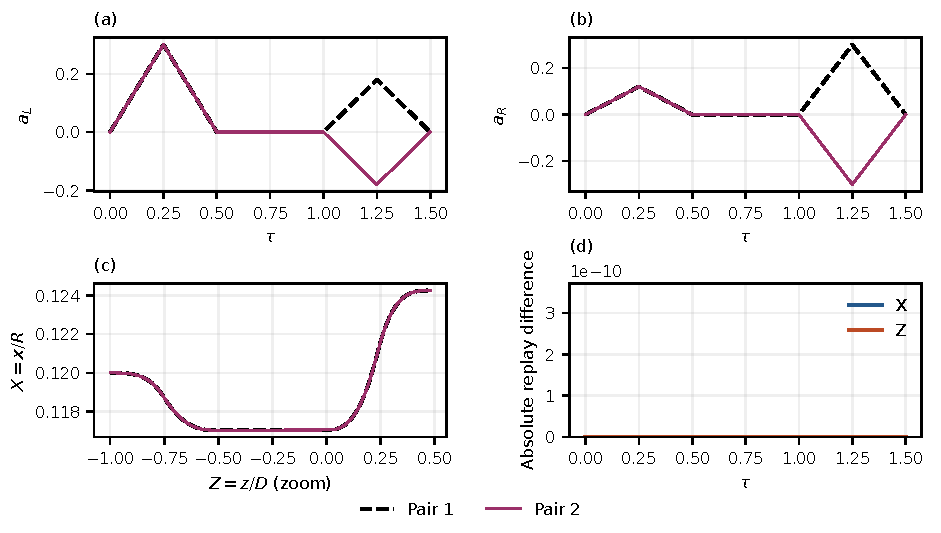
\includegraphics[width=0.98\textwidth]{figs/chapter4/inverse-master10-ambiguity.pdf}
% REVIEW-TERM T13 | فاصلهٔ صفر | همان ابهام T12 در معرفی شکل و عنوان آن تکرار شده است. فقط عبارت مربوط در عنوان هایلایت شود؛ تصویر دست‌نخورده بماند. | پیشنهاد: بازهٔ زمانی با تحریک صفر در هر دو منبع | رفع ابهام در متن و عنوان شکل؛ اطمینان بالا | کد، صفر مشترکِ زمانی را میان دو پالس اعمال می‌کند.؛ مرتبط Y44
% REVIEW-AUDIT Y44 | تحریک‌های متفاوت پس از فاصلهٔ صفر و مسیرهای مستقل هم‌پوشان | فرمان‌های متفاوت می‌توانند مسیر فیزیکی یکسان ایجاد کنند. | پیشنهاد: ابهام علامت پس از بازهٔ صفر مشترک | مرور؛ محدودیت ساختاری شناسایی‌پذیری | هر دو تحریک در چند گرهٔ متوالی صفرند. علامت پالس دوم برای هر دو عوض می‌شود.؛ مرتبط T13
\caption{\ReviewMark{yellow}{Y44-834-2-1}{تحریک‌های متفاوت پس از} \ReviewMark{blue}{T13-834-1-1}{فاصلهٔ صفر} \ReviewMark{yellow}{Y44-834-2-3}{و مسیرهای مستقل هم‌پوشان}.}
\label{fig:results-master10-ambiguity}
\end{figure}
